\documentclass[twoside]{book}

% Packages required by doxygen
\usepackage{fixltx2e}
\usepackage{calc}
\usepackage{doxygen}
\usepackage[export]{adjustbox} % also loads graphicx
\usepackage{graphicx}
\usepackage[utf8]{inputenc}
\usepackage{makeidx}
\usepackage{multicol}
\usepackage{multirow}
\PassOptionsToPackage{warn}{textcomp}
\usepackage{textcomp}
\usepackage[nointegrals]{wasysym}
\usepackage[table]{xcolor}

% Font selection
\usepackage[T1]{fontenc}
\usepackage[scaled=.90]{helvet}
\usepackage{courier}
\usepackage{amssymb}
\usepackage{sectsty}
\renewcommand{\familydefault}{\sfdefault}
\allsectionsfont{%
  \fontseries{bc}\selectfont%
  \color{darkgray}%
}
\renewcommand{\DoxyLabelFont}{%
  \fontseries{bc}\selectfont%
  \color{darkgray}%
}
\newcommand{\+}{\discretionary{\mbox{\scriptsize$\hookleftarrow$}}{}{}}

% Page & text layout
\usepackage{geometry}
\geometry{%
  a4paper,%
  top=2.5cm,%
  bottom=2.5cm,%
  left=2.5cm,%
  right=2.5cm%
}
\tolerance=750
\hfuzz=15pt
\hbadness=750
\setlength{\emergencystretch}{15pt}
\setlength{\parindent}{0cm}
\setlength{\parskip}{3ex plus 2ex minus 2ex}
\makeatletter
\renewcommand{\paragraph}{%
  \@startsection{paragraph}{4}{0ex}{-1.0ex}{1.0ex}{%
    \normalfont\normalsize\bfseries\SS@parafont%
  }%
}
\renewcommand{\subparagraph}{%
  \@startsection{subparagraph}{5}{0ex}{-1.0ex}{1.0ex}{%
    \normalfont\normalsize\bfseries\SS@subparafont%
  }%
}
\makeatother

% Headers & footers
\usepackage{fancyhdr}
\pagestyle{fancyplain}
\fancyhead[LE]{\fancyplain{}{\bfseries\thepage}}
\fancyhead[CE]{\fancyplain{}{}}
\fancyhead[RE]{\fancyplain{}{\bfseries\leftmark}}
\fancyhead[LO]{\fancyplain{}{\bfseries\rightmark}}
\fancyhead[CO]{\fancyplain{}{}}
\fancyhead[RO]{\fancyplain{}{\bfseries\thepage}}
\fancyfoot[LE]{\fancyplain{}{}}
\fancyfoot[CE]{\fancyplain{}{}}
\fancyfoot[RE]{\fancyplain{}{\bfseries\scriptsize Generated by Doxygen }}
\fancyfoot[LO]{\fancyplain{}{\bfseries\scriptsize Generated by Doxygen }}
\fancyfoot[CO]{\fancyplain{}{}}
\fancyfoot[RO]{\fancyplain{}{}}
\renewcommand{\footrulewidth}{0.4pt}
\renewcommand{\chaptermark}[1]{%
  \markboth{#1}{}%
}
\renewcommand{\sectionmark}[1]{%
  \markright{\thesection\ #1}%
}

% Indices & bibliography
\usepackage{natbib}
\usepackage[titles]{tocloft}
\setcounter{tocdepth}{3}
\setcounter{secnumdepth}{5}
\makeindex

% Hyperlinks (required, but should be loaded last)
\usepackage{ifpdf}
\ifpdf
  \usepackage[pdftex,pagebackref=true]{hyperref}
\else
  \usepackage[ps2pdf,pagebackref=true]{hyperref}
\fi
\hypersetup{%
  colorlinks=true,%
  linkcolor=blue,%
  citecolor=blue,%
  unicode%
}

% Custom commands
\newcommand{\clearemptydoublepage}{%
  \newpage{\pagestyle{empty}\cleardoublepage}%
}

\usepackage{caption}
\captionsetup{labelsep=space,justification=centering,font={bf},singlelinecheck=off,skip=4pt,position=top}

%===== C O N T E N T S =====

\begin{document}

% Titlepage & ToC
\hypersetup{pageanchor=false,
             bookmarksnumbered=true,
             pdfencoding=unicode
            }
\pagenumbering{roman}
\begin{titlepage}
\vspace*{7cm}
\begin{center}%
{\Large Gomoku }\\
\vspace*{1cm}
{\large Generated by Doxygen 1.8.11}\\
\end{center}
\end{titlepage}
\clearemptydoublepage
\tableofcontents
\clearemptydoublepage
\pagenumbering{arabic}
\hypersetup{pageanchor=true}

%--- Begin generated contents ---
\chapter{Namespace Index}
\section{Namespace List}
Here is a list of all namespaces with brief descriptions\+:\begin{DoxyCompactList}
\item\contentsline{section}{\hyperlink{namespaceUi}{Ui} }{\pageref{namespaceUi}}{}
\end{DoxyCompactList}

\chapter{Hierarchical Index}
\section{Class Hierarchy}
This inheritance list is sorted roughly, but not completely, alphabetically\+:\begin{DoxyCompactList}
\item Q\+Dialog\begin{DoxyCompactList}
\item \contentsline{section}{Ip\+Input}{\pageref{classIpInput}}{}
\item \contentsline{section}{Server\+Dialog}{\pageref{classServerDialog}}{}
\end{DoxyCompactList}
\item Q\+Main\+Window\begin{DoxyCompactList}
\item \contentsline{section}{Gomoku}{\pageref{classGomoku}}{}
\end{DoxyCompactList}
\item Q\+Object\begin{DoxyCompactList}
\item \contentsline{section}{Board}{\pageref{classBoard}}{}
\item \contentsline{section}{Data}{\pageref{classData}}{}
\item \contentsline{section}{Getter}{\pageref{classGetter}}{}
\item \contentsline{section}{Input}{\pageref{classInput}}{}
\begin{DoxyCompactList}
\item \contentsline{section}{Remote\+Input}{\pageref{classRemoteInput}}{}
\end{DoxyCompactList}
\end{DoxyCompactList}
\item Q\+Widget\begin{DoxyCompactList}
\item \contentsline{section}{Cross}{\pageref{classCross}}{}
\end{DoxyCompactList}
\end{DoxyCompactList}

\chapter{Class Index}
\section{Class List}
Here are the classes, structs, unions and interfaces with brief descriptions\+:\begin{DoxyCompactList}
\item\contentsline{section}{\hyperlink{classBoard}{Board} \\*\hyperlink{classGomoku}{Gomoku} board }{\pageref{classBoard}}{}
\item\contentsline{section}{\hyperlink{classCross}{Cross} \\*A \hyperlink{classCross}{Cross} on the board }{\pageref{classCross}}{}
\item\contentsline{section}{\hyperlink{classData}{Data} \\*Manages all data }{\pageref{classData}}{}
\item\contentsline{section}{\hyperlink{classGetter}{Getter} }{\pageref{classGetter}}{}
\item\contentsline{section}{\hyperlink{classGomoku}{Gomoku} \\*Main window }{\pageref{classGomoku}}{}
\item\contentsline{section}{\hyperlink{classInput}{Input} \\*Base class for user input from local or remote }{\pageref{classInput}}{}
\item\contentsline{section}{\hyperlink{classIpInput}{Ip\+Input} }{\pageref{classIpInput}}{}
\item\contentsline{section}{\hyperlink{classRemoteInput}{Remote\+Input} \\*User input from remote }{\pageref{classRemoteInput}}{}
\item\contentsline{section}{\hyperlink{classServerDialog}{Server\+Dialog} \\*Dialog to setup a server }{\pageref{classServerDialog}}{}
\end{DoxyCompactList}

\chapter{File Index}
\section{File List}
Here is a list of all files with brief descriptions\+:\begin{DoxyCompactList}
\item\contentsline{section}{\hyperlink{board_8cpp}{board.\+cpp} }{\pageref{board_8cpp}}{}
\item\contentsline{section}{\hyperlink{board_8h}{board.\+h} }{\pageref{board_8h}}{}
\item\contentsline{section}{\hyperlink{const_8h}{const.\+h} }{\pageref{const_8h}}{}
\item\contentsline{section}{\hyperlink{cross_8cpp}{cross.\+cpp} }{\pageref{cross_8cpp}}{}
\item\contentsline{section}{\hyperlink{cross_8h}{cross.\+h} }{\pageref{cross_8h}}{}
\item\contentsline{section}{\hyperlink{data_8cpp}{data.\+cpp} }{\pageref{data_8cpp}}{}
\item\contentsline{section}{\hyperlink{data_8h}{data.\+h} }{\pageref{data_8h}}{}
\item\contentsline{section}{\hyperlink{gomoku_8cpp}{gomoku.\+cpp} }{\pageref{gomoku_8cpp}}{}
\item\contentsline{section}{\hyperlink{gomoku_8h}{gomoku.\+h} }{\pageref{gomoku_8h}}{}
\item\contentsline{section}{\hyperlink{input_8cpp}{input.\+cpp} }{\pageref{input_8cpp}}{}
\item\contentsline{section}{\hyperlink{input_8h}{input.\+h} }{\pageref{input_8h}}{}
\item\contentsline{section}{\hyperlink{ipinput_8cpp}{ipinput.\+cpp} }{\pageref{ipinput_8cpp}}{}
\item\contentsline{section}{\hyperlink{ipinput_8h}{ipinput.\+h} }{\pageref{ipinput_8h}}{}
\item\contentsline{section}{\hyperlink{main_8cpp}{main.\+cpp} }{\pageref{main_8cpp}}{}
\item\contentsline{section}{\hyperlink{remoteinput_8cpp}{remoteinput.\+cpp} }{\pageref{remoteinput_8cpp}}{}
\item\contentsline{section}{\hyperlink{remoteinput_8h}{remoteinput.\+h} }{\pageref{remoteinput_8h}}{}
\item\contentsline{section}{\hyperlink{serverdialog_8cpp}{serverdialog.\+cpp} }{\pageref{serverdialog_8cpp}}{}
\item\contentsline{section}{\hyperlink{serverdialog_8h}{serverdialog.\+h} }{\pageref{serverdialog_8h}}{}
\end{DoxyCompactList}

\chapter{Namespace Documentation}
\hypertarget{namespaceUi}{}\section{Ui Namespace Reference}
\label{namespaceUi}\index{Ui@{Ui}}

\chapter{Class Documentation}
\hypertarget{classBoard}{}\section{Board Class Reference}
\label{classBoard}\index{Board@{Board}}


\hyperlink{classGomoku}{Gomoku} board.  




{\ttfamily \#include $<$board.\+h$>$}



Inheritance diagram for Board\+:
\nopagebreak
\begin{figure}[H]
\begin{center}
\leavevmode
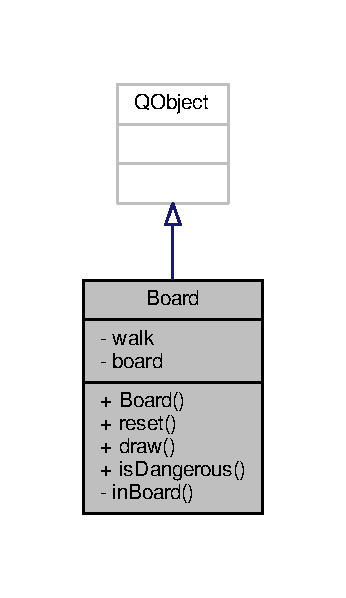
\includegraphics[width=166pt]{classBoard__inherit__graph}
\end{center}
\end{figure}


Collaboration diagram for Board\+:
\nopagebreak
\begin{figure}[H]
\begin{center}
\leavevmode
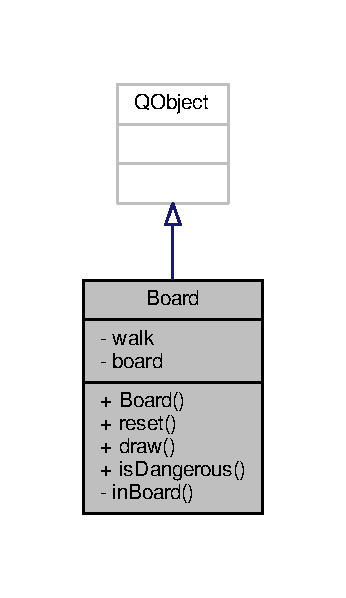
\includegraphics[width=166pt]{classBoard__coll__graph}
\end{center}
\end{figure}
\subsection*{Signals}
\begin{DoxyCompactItemize}
\item 
void \hyperlink{classBoard_ac3725569d7c112f0fbf8fc9a4aee1477}{win} (bool color)
\end{DoxyCompactItemize}
\subsection*{Public Member Functions}
\begin{DoxyCompactItemize}
\item 
\hyperlink{classBoard_a40471004facb958cf0e60840cd441ab8}{Board} (Q\+Object $\ast$parent=0)
\item 
void \hyperlink{classBoard_aaef819a8d1a10c35d9f802195802236e}{reset} ()
\item 
void \hyperlink{classBoard_a9d29e2f76551363e49e93467f7ca7ece}{draw} (int row, int column, bool color)
\item 
bool \hyperlink{classBoard_aec12d14fa7095b68e176dd7c6e8bf73b}{is\+Dangerous} (int row, int column, bool color)
\begin{DoxyCompactList}\small\item\em is dangerous for color {\ttfamily color} \end{DoxyCompactList}\end{DoxyCompactItemize}
\subsection*{Private Member Functions}
\begin{DoxyCompactItemize}
\item 
bool \hyperlink{classBoard_a2f339d1294177dc9cb1a0c160b1427f5}{in\+Board} (int row, int column)
\end{DoxyCompactItemize}
\subsection*{Private Attributes}
\begin{DoxyCompactItemize}
\item 
const int \hyperlink{classBoard_a362b986e66494ee079a6dd2b8b08075f}{walk} \mbox{[}8\mbox{]}\mbox{[}2\mbox{]} = \{\{-\/1,0\}, \{-\/1,1\}, \{0,1\}, \{1,1\}, \{1,0\}, \{1,-\/1\}, \{0,-\/1\}, \{-\/1,-\/1\}\}
\item 
int \hyperlink{classBoard_af4a66521596ff3eef6685b7e15438977}{board} \mbox{[}\hyperlink{const_8h_aa7a2b8ea2c784a4ad8b58a3262bb4f07}{B\+O\+A\+R\+D\+\_\+\+S\+I\+ZE}\mbox{]}\mbox{[}\hyperlink{const_8h_aa7a2b8ea2c784a4ad8b58a3262bb4f07}{B\+O\+A\+R\+D\+\_\+\+S\+I\+ZE}\mbox{]}
\end{DoxyCompactItemize}


\subsection{Detailed Description}
\hyperlink{classGomoku}{Gomoku} board. 

\subsection{Constructor \& Destructor Documentation}
\index{Board@{Board}!Board@{Board}}
\index{Board@{Board}!Board@{Board}}
\subsubsection[{\texorpdfstring{Board(\+Q\+Object $\ast$parent=0)}{Board(QObject *parent=0)}}]{\setlength{\rightskip}{0pt plus 5cm}Board\+::\+Board (
\begin{DoxyParamCaption}
\item[{Q\+Object $\ast$}]{parent = {\ttfamily 0}}
\end{DoxyParamCaption}
)\hspace{0.3cm}{\ttfamily [explicit]}}\hypertarget{classBoard_a40471004facb958cf0e60840cd441ab8}{}\label{classBoard_a40471004facb958cf0e60840cd441ab8}


\subsection{Member Function Documentation}
\index{Board@{Board}!draw@{draw}}
\index{draw@{draw}!Board@{Board}}
\subsubsection[{\texorpdfstring{draw(int row, int column, bool color)}{draw(int row, int column, bool color)}}]{\setlength{\rightskip}{0pt plus 5cm}void Board\+::draw (
\begin{DoxyParamCaption}
\item[{int}]{row, }
\item[{int}]{column, }
\item[{bool}]{color}
\end{DoxyParamCaption}
)}\hypertarget{classBoard_a9d29e2f76551363e49e93467f7ca7ece}{}\label{classBoard_a9d29e2f76551363e49e93467f7ca7ece}
\index{Board@{Board}!in\+Board@{in\+Board}}
\index{in\+Board@{in\+Board}!Board@{Board}}
\subsubsection[{\texorpdfstring{in\+Board(int row, int column)}{inBoard(int row, int column)}}]{\setlength{\rightskip}{0pt plus 5cm}bool Board\+::in\+Board (
\begin{DoxyParamCaption}
\item[{int}]{row, }
\item[{int}]{column}
\end{DoxyParamCaption}
)\hspace{0.3cm}{\ttfamily [private]}}\hypertarget{classBoard_a2f339d1294177dc9cb1a0c160b1427f5}{}\label{classBoard_a2f339d1294177dc9cb1a0c160b1427f5}
\index{Board@{Board}!is\+Dangerous@{is\+Dangerous}}
\index{is\+Dangerous@{is\+Dangerous}!Board@{Board}}
\subsubsection[{\texorpdfstring{is\+Dangerous(int row, int column, bool color)}{isDangerous(int row, int column, bool color)}}]{\setlength{\rightskip}{0pt plus 5cm}bool Board\+::is\+Dangerous (
\begin{DoxyParamCaption}
\item[{int}]{row, }
\item[{int}]{column, }
\item[{bool}]{color}
\end{DoxyParamCaption}
)}\hypertarget{classBoard_aec12d14fa7095b68e176dd7c6e8bf73b}{}\label{classBoard_aec12d14fa7095b68e176dd7c6e8bf73b}


is dangerous for color {\ttfamily color} 

\index{Board@{Board}!reset@{reset}}
\index{reset@{reset}!Board@{Board}}
\subsubsection[{\texorpdfstring{reset()}{reset()}}]{\setlength{\rightskip}{0pt plus 5cm}void Board\+::reset (
\begin{DoxyParamCaption}
{}
\end{DoxyParamCaption}
)}\hypertarget{classBoard_aaef819a8d1a10c35d9f802195802236e}{}\label{classBoard_aaef819a8d1a10c35d9f802195802236e}
\index{Board@{Board}!win@{win}}
\index{win@{win}!Board@{Board}}
\subsubsection[{\texorpdfstring{win}{win}}]{\setlength{\rightskip}{0pt plus 5cm}void Board\+::win (
\begin{DoxyParamCaption}
\item[{bool}]{color}
\end{DoxyParamCaption}
)\hspace{0.3cm}{\ttfamily [signal]}}\hypertarget{classBoard_ac3725569d7c112f0fbf8fc9a4aee1477}{}\label{classBoard_ac3725569d7c112f0fbf8fc9a4aee1477}


\subsection{Member Data Documentation}
\index{Board@{Board}!board@{board}}
\index{board@{board}!Board@{Board}}
\subsubsection[{\texorpdfstring{board}{board}}]{\setlength{\rightskip}{0pt plus 5cm}int Board\+::board\mbox{[}{\bf B\+O\+A\+R\+D\+\_\+\+S\+I\+ZE}\mbox{]}\mbox{[}{\bf B\+O\+A\+R\+D\+\_\+\+S\+I\+ZE}\mbox{]}\hspace{0.3cm}{\ttfamily [private]}}\hypertarget{classBoard_af4a66521596ff3eef6685b7e15438977}{}\label{classBoard_af4a66521596ff3eef6685b7e15438977}
\index{Board@{Board}!walk@{walk}}
\index{walk@{walk}!Board@{Board}}
\subsubsection[{\texorpdfstring{walk}{walk}}]{\setlength{\rightskip}{0pt plus 5cm}const int Board\+::walk\mbox{[}8\mbox{]}\mbox{[}2\mbox{]} = \{\{-\/1,0\}, \{-\/1,1\}, \{0,1\}, \{1,1\}, \{1,0\}, \{1,-\/1\}, \{0,-\/1\}, \{-\/1,-\/1\}\}\hspace{0.3cm}{\ttfamily [private]}}\hypertarget{classBoard_a362b986e66494ee079a6dd2b8b08075f}{}\label{classBoard_a362b986e66494ee079a6dd2b8b08075f}


The documentation for this class was generated from the following files\+:\begin{DoxyCompactItemize}
\item 
\hyperlink{board_8h}{board.\+h}\item 
\hyperlink{board_8cpp}{board.\+cpp}\end{DoxyCompactItemize}

\hypertarget{classCross}{}\section{Cross Class Reference}
\label{classCross}\index{Cross@{Cross}}


A \hyperlink{classCross}{Cross} on the board.  




{\ttfamily \#include $<$cross.\+h$>$}



Inheritance diagram for Cross\+:
\nopagebreak
\begin{figure}[H]
\begin{center}
\leavevmode
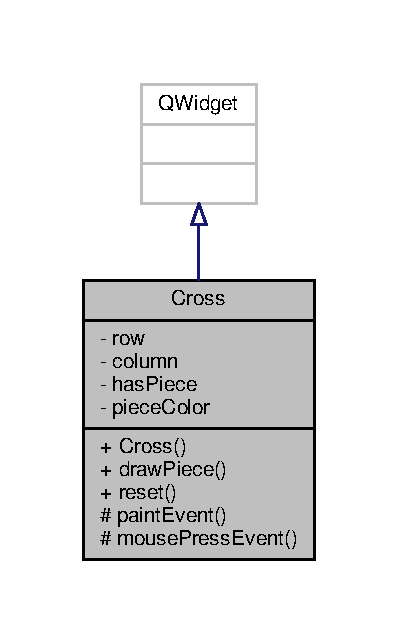
\includegraphics[width=191pt]{classCross__inherit__graph}
\end{center}
\end{figure}


Collaboration diagram for Cross\+:
\nopagebreak
\begin{figure}[H]
\begin{center}
\leavevmode
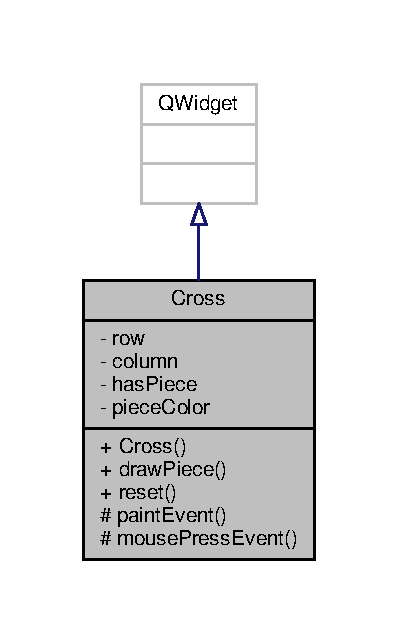
\includegraphics[width=191pt]{classCross__coll__graph}
\end{center}
\end{figure}
\subsection*{Signals}
\begin{DoxyCompactItemize}
\item 
void \hyperlink{classCross_a3236a3d5b8df5df8360991c3c2c84151}{on\+Click} (int \+\_\+row, int \+\_\+column)
\end{DoxyCompactItemize}
\subsection*{Public Member Functions}
\begin{DoxyCompactItemize}
\item 
\hyperlink{classCross_a2c8a7e6d5023308aad6cf6adc03bcd40}{Cross} (int \+\_\+row, int \+\_\+column, Q\+Widget $\ast$parent)
\item 
void \hyperlink{classCross_a7a9c22df3681abcdf297ff6eae640f0a}{draw\+Piece} (bool color)
\item 
void \hyperlink{classCross_ae748d570f5e5a1e3427bd5866cc44118}{reset} ()
\end{DoxyCompactItemize}
\subsection*{Protected Member Functions}
\begin{DoxyCompactItemize}
\item 
void \hyperlink{classCross_ad12f50256807ced47283f96e4aebf997}{paint\+Event} (Q\+Paint\+Event $\ast$event) override
\item 
void \hyperlink{classCross_a45673e2233d66b8b094ddf201948cd98}{mouse\+Press\+Event} (Q\+Mouse\+Event $\ast$event) override
\end{DoxyCompactItemize}
\subsection*{Private Attributes}
\begin{DoxyCompactItemize}
\item 
int \hyperlink{classCross_a21935454e9ea07a0f2ec0bfe9338622c}{row}
\item 
int \hyperlink{classCross_a618536d0ef3121b0e2a8d74737e1a00c}{column}
\item 
bool \hyperlink{classCross_aa8369e751da4a7910bb552242ac19092}{has\+Piece}
\item 
bool \hyperlink{classCross_a7ed2b797ef98393f7096acda24e7e38f}{piece\+Color}
\end{DoxyCompactItemize}


\subsection{Detailed Description}
A \hyperlink{classCross}{Cross} on the board. 

\subsection{Constructor \& Destructor Documentation}
\index{Cross@{Cross}!Cross@{Cross}}
\index{Cross@{Cross}!Cross@{Cross}}
\subsubsection[{\texorpdfstring{Cross(int \+\_\+row, int \+\_\+column, Q\+Widget $\ast$parent)}{Cross(int _row, int _column, QWidget *parent)}}]{\setlength{\rightskip}{0pt plus 5cm}Cross\+::\+Cross (
\begin{DoxyParamCaption}
\item[{int}]{\+\_\+row, }
\item[{int}]{\+\_\+column, }
\item[{Q\+Widget $\ast$}]{parent}
\end{DoxyParamCaption}
)\hspace{0.3cm}{\ttfamily [explicit]}}\hypertarget{classCross_a2c8a7e6d5023308aad6cf6adc03bcd40}{}\label{classCross_a2c8a7e6d5023308aad6cf6adc03bcd40}


\subsection{Member Function Documentation}
\index{Cross@{Cross}!draw\+Piece@{draw\+Piece}}
\index{draw\+Piece@{draw\+Piece}!Cross@{Cross}}
\subsubsection[{\texorpdfstring{draw\+Piece(bool color)}{drawPiece(bool color)}}]{\setlength{\rightskip}{0pt plus 5cm}void Cross\+::draw\+Piece (
\begin{DoxyParamCaption}
\item[{bool}]{color}
\end{DoxyParamCaption}
)\hspace{0.3cm}{\ttfamily [inline]}}\hypertarget{classCross_a7a9c22df3681abcdf297ff6eae640f0a}{}\label{classCross_a7a9c22df3681abcdf297ff6eae640f0a}
\index{Cross@{Cross}!mouse\+Press\+Event@{mouse\+Press\+Event}}
\index{mouse\+Press\+Event@{mouse\+Press\+Event}!Cross@{Cross}}
\subsubsection[{\texorpdfstring{mouse\+Press\+Event(\+Q\+Mouse\+Event $\ast$event) override}{mousePressEvent(QMouseEvent *event) override}}]{\setlength{\rightskip}{0pt plus 5cm}void Cross\+::mouse\+Press\+Event (
\begin{DoxyParamCaption}
\item[{Q\+Mouse\+Event $\ast$}]{event}
\end{DoxyParamCaption}
)\hspace{0.3cm}{\ttfamily [override]}, {\ttfamily [protected]}}\hypertarget{classCross_a45673e2233d66b8b094ddf201948cd98}{}\label{classCross_a45673e2233d66b8b094ddf201948cd98}
\index{Cross@{Cross}!on\+Click@{on\+Click}}
\index{on\+Click@{on\+Click}!Cross@{Cross}}
\subsubsection[{\texorpdfstring{on\+Click}{onClick}}]{\setlength{\rightskip}{0pt plus 5cm}void Cross\+::on\+Click (
\begin{DoxyParamCaption}
\item[{int}]{\+\_\+row, }
\item[{int}]{\+\_\+column}
\end{DoxyParamCaption}
)\hspace{0.3cm}{\ttfamily [signal]}}\hypertarget{classCross_a3236a3d5b8df5df8360991c3c2c84151}{}\label{classCross_a3236a3d5b8df5df8360991c3c2c84151}
\index{Cross@{Cross}!paint\+Event@{paint\+Event}}
\index{paint\+Event@{paint\+Event}!Cross@{Cross}}
\subsubsection[{\texorpdfstring{paint\+Event(\+Q\+Paint\+Event $\ast$event) override}{paintEvent(QPaintEvent *event) override}}]{\setlength{\rightskip}{0pt plus 5cm}void Cross\+::paint\+Event (
\begin{DoxyParamCaption}
\item[{Q\+Paint\+Event $\ast$}]{event}
\end{DoxyParamCaption}
)\hspace{0.3cm}{\ttfamily [override]}, {\ttfamily [protected]}}\hypertarget{classCross_ad12f50256807ced47283f96e4aebf997}{}\label{classCross_ad12f50256807ced47283f96e4aebf997}
\index{Cross@{Cross}!reset@{reset}}
\index{reset@{reset}!Cross@{Cross}}
\subsubsection[{\texorpdfstring{reset()}{reset()}}]{\setlength{\rightskip}{0pt plus 5cm}void Cross\+::reset (
\begin{DoxyParamCaption}
{}
\end{DoxyParamCaption}
)\hspace{0.3cm}{\ttfamily [inline]}}\hypertarget{classCross_ae748d570f5e5a1e3427bd5866cc44118}{}\label{classCross_ae748d570f5e5a1e3427bd5866cc44118}


\subsection{Member Data Documentation}
\index{Cross@{Cross}!column@{column}}
\index{column@{column}!Cross@{Cross}}
\subsubsection[{\texorpdfstring{column}{column}}]{\setlength{\rightskip}{0pt plus 5cm}int Cross\+::column\hspace{0.3cm}{\ttfamily [private]}}\hypertarget{classCross_a618536d0ef3121b0e2a8d74737e1a00c}{}\label{classCross_a618536d0ef3121b0e2a8d74737e1a00c}
\index{Cross@{Cross}!has\+Piece@{has\+Piece}}
\index{has\+Piece@{has\+Piece}!Cross@{Cross}}
\subsubsection[{\texorpdfstring{has\+Piece}{hasPiece}}]{\setlength{\rightskip}{0pt plus 5cm}bool Cross\+::has\+Piece\hspace{0.3cm}{\ttfamily [private]}}\hypertarget{classCross_aa8369e751da4a7910bb552242ac19092}{}\label{classCross_aa8369e751da4a7910bb552242ac19092}
\index{Cross@{Cross}!piece\+Color@{piece\+Color}}
\index{piece\+Color@{piece\+Color}!Cross@{Cross}}
\subsubsection[{\texorpdfstring{piece\+Color}{pieceColor}}]{\setlength{\rightskip}{0pt plus 5cm}bool Cross\+::piece\+Color\hspace{0.3cm}{\ttfamily [private]}}\hypertarget{classCross_a7ed2b797ef98393f7096acda24e7e38f}{}\label{classCross_a7ed2b797ef98393f7096acda24e7e38f}
\index{Cross@{Cross}!row@{row}}
\index{row@{row}!Cross@{Cross}}
\subsubsection[{\texorpdfstring{row}{row}}]{\setlength{\rightskip}{0pt plus 5cm}int Cross\+::row\hspace{0.3cm}{\ttfamily [private]}}\hypertarget{classCross_a21935454e9ea07a0f2ec0bfe9338622c}{}\label{classCross_a21935454e9ea07a0f2ec0bfe9338622c}


The documentation for this class was generated from the following files\+:\begin{DoxyCompactItemize}
\item 
\hyperlink{cross_8h}{cross.\+h}\item 
\hyperlink{cross_8cpp}{cross.\+cpp}\end{DoxyCompactItemize}

\hypertarget{classData}{}\section{Data Class Reference}
\label{classData}\index{Data@{Data}}


Manages all data.  




{\ttfamily \#include $<$data.\+h$>$}



Inheritance diagram for Data\+:
\nopagebreak
\begin{figure}[H]
\begin{center}
\leavevmode
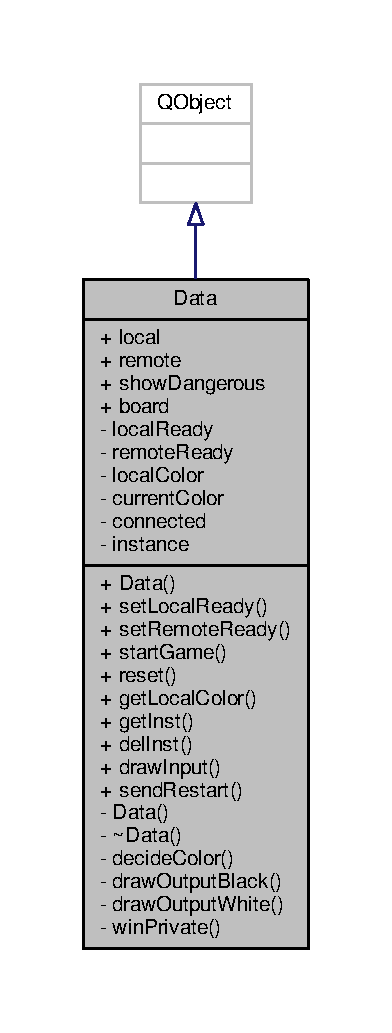
\includegraphics[width=188pt]{classData__inherit__graph}
\end{center}
\end{figure}


Collaboration diagram for Data\+:
\nopagebreak
\begin{figure}[H]
\begin{center}
\leavevmode
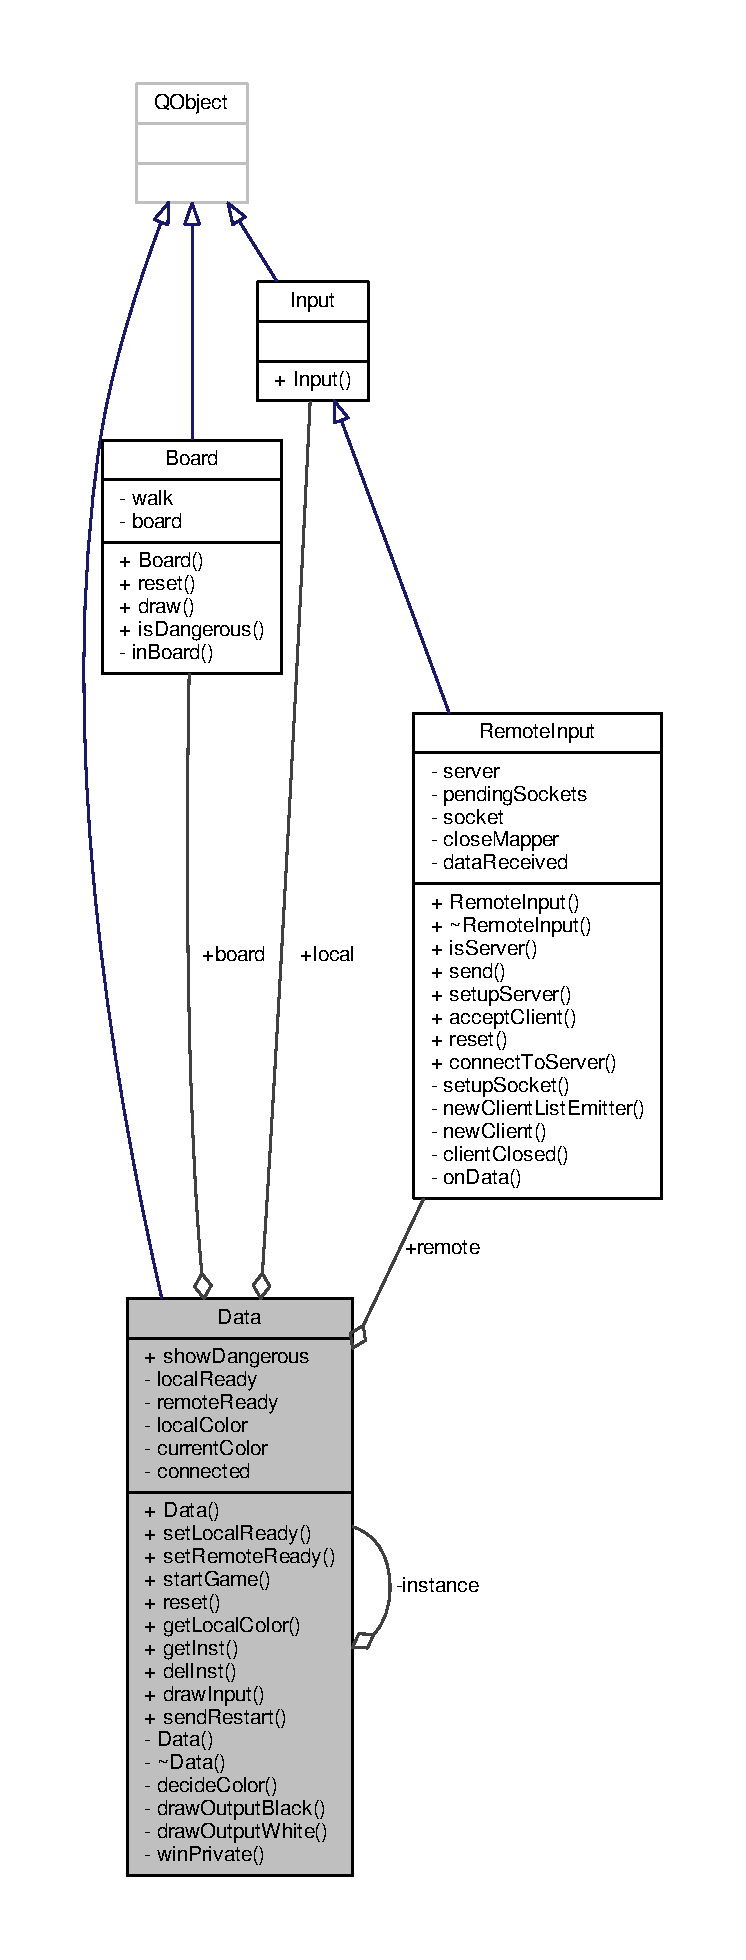
\includegraphics[height=550pt]{classData__coll__graph}
\end{center}
\end{figure}
\subsection*{Public Slots}
\begin{DoxyCompactItemize}
\item 
void \hyperlink{classData_acc4edfbc7e9cfdf810d01e404b0129de}{draw\+Input} (int row, int column)
\begin{DoxyCompactList}\small\item\em input draw from user \end{DoxyCompactList}\item 
void \hyperlink{classData_aa54baf049c35f1ac45db3b2c9c6b42bf}{send\+Restart} ()
\begin{DoxyCompactList}\small\item\em tell remote to restart \end{DoxyCompactList}\end{DoxyCompactItemize}
\subsection*{Signals}
\begin{DoxyCompactItemize}
\item 
void \hyperlink{classData_a2ff062f4a7867e73c080f6f001cc074a}{draw\+Output} (int row, int column, bool color)
\begin{DoxyCompactList}\small\item\em output draw to board \end{DoxyCompactList}\item 
void \hyperlink{classData_a2331d231b898355973181c02c6a53042}{win} (bool color)
\begin{DoxyCompactList}\small\item\em A color wins. \end{DoxyCompactList}\end{DoxyCompactItemize}
\subsection*{Public Member Functions}
\begin{DoxyCompactItemize}
\item 
\hyperlink{classData_abcae162153c8d0a55bb89919f5ccba03}{Data} (const \hyperlink{classData}{Data} \&)=delete
\item 
void \hyperlink{classData_aeb1e91a5f2ce9d978a28d1aed4ac46c2}{set\+Local\+Ready} ()
\begin{DoxyCompactList}\small\item\em set as ready to play \end{DoxyCompactList}\item 
void \hyperlink{classData_ab2b27bfac830989abd87c2cc2f188d53}{set\+Remote\+Ready} ()
\item 
void \hyperlink{classData_a8db5b20b0fe960b7f13819d59a5a1a09}{start\+Game} (bool color)
\begin{DoxyCompactList}\small\item\em set local color and start game \end{DoxyCompactList}\item 
void \hyperlink{classData_ae974ac11bbc2330fb43c9bb03f60f3cf}{reset} ()
\begin{DoxyCompactList}\small\item\em clear board and reset color \end{DoxyCompactList}\item 
bool \hyperlink{classData_a57c47976e11427223f0f18e99f19a09f}{get\+Local\+Color} ()
\end{DoxyCompactItemize}
\subsection*{Static Public Member Functions}
\begin{DoxyCompactItemize}
\item 
static \hyperlink{classData}{Data} $\ast$ \hyperlink{classData_ad35a80f2a296e08d9ff81444566570f5}{get\+Inst} ()
\begin{DoxyCompactList}\small\item\em Get singleton instance. \end{DoxyCompactList}\item 
static void \hyperlink{classData_a28e9f57b4cff7a6fe1058defc0ccac08}{del\+Inst} ()
\begin{DoxyCompactList}\small\item\em Remove instance. \end{DoxyCompactList}\end{DoxyCompactItemize}
\subsection*{Public Attributes}
\begin{DoxyCompactItemize}
\item 
\hyperlink{classInput}{Input} $\ast$ \hyperlink{classData_a66242713cb93b680f847231ee57457bd}{local}
\begin{DoxyCompactList}\small\item\em local player \end{DoxyCompactList}\item 
\hyperlink{classRemoteInput}{Remote\+Input} $\ast$ \hyperlink{classData_ab1b9a7098b7d41fdab0366b2a9c660ed}{remote}
\begin{DoxyCompactList}\small\item\em remote player \end{DoxyCompactList}\item 
bool \hyperlink{classData_a2909d285f3adfe5a61c8ea181cd7824c}{show\+Dangerous}
\item 
\hyperlink{classBoard}{Board} \hyperlink{classData_aa932fae932d34b82666a9b56e1c36f8c}{board}
\end{DoxyCompactItemize}
\subsection*{Private Slots}
\begin{DoxyCompactItemize}
\item 
void \hyperlink{classData_a85f3f284e7f73ab815b2dd2cd10d774f}{draw\+Output\+Black} (int row, int column)
\item 
void \hyperlink{classData_add002ff89ac45f63df4dfe2f873d5756}{draw\+Output\+White} (int row, int column)
\item 
void \hyperlink{classData_a5272d4ddc3263564cd13f47d609ab8b8}{win\+Private} (bool color)
\end{DoxyCompactItemize}
\subsection*{Private Member Functions}
\begin{DoxyCompactItemize}
\item 
\hyperlink{classData_a1eaf44e85889a39a1263db2172162530}{Data} (Q\+Object $\ast$parent=0)
\item 
\hyperlink{classData_aab31956423290f0d62dcca47ab4d16dd}{$\sim$\+Data} ()
\item 
void \hyperlink{classData_ae73f56bd8100715a1c2fa0765f5bfd25}{decide\+Color} ()
\begin{DoxyCompactList}\small\item\em decide color and tell remote side \end{DoxyCompactList}\end{DoxyCompactItemize}
\subsection*{Private Attributes}
\begin{DoxyCompactItemize}
\item 
bool \hyperlink{classData_aba43b573b14a94fa8798b76e92aa2db2}{local\+Ready}
\item 
bool \hyperlink{classData_a611e221f2d956e25eee03fc88d2bd453}{remote\+Ready}
\item 
bool \hyperlink{classData_a5530c3c349903bb4f6b3c95223de40ad}{local\+Color}
\item 
bool \hyperlink{classData_a78b5ab819236924f1699f83f0eafc0d2}{current\+Color}
\item 
bool \hyperlink{classData_adc0eab5a1c090fa044827e957c5d06f9}{connected}
\begin{DoxyCompactList}\small\item\em connected signal draw to slot draw\+Output\+Black/\+White \end{DoxyCompactList}\end{DoxyCompactItemize}
\subsection*{Static Private Attributes}
\begin{DoxyCompactItemize}
\item 
static \hyperlink{classData}{Data} $\ast$ \hyperlink{classData_ad373f0e9d46abaf2e67a6c40d4510d29}{instance} = 0
\end{DoxyCompactItemize}


\subsection{Detailed Description}
Manages all data. 

\subsection{Constructor \& Destructor Documentation}
\index{Data@{Data}!Data@{Data}}
\index{Data@{Data}!Data@{Data}}
\subsubsection[{\texorpdfstring{Data(const Data \&)=delete}{Data(const Data &)=delete}}]{\setlength{\rightskip}{0pt plus 5cm}Data\+::\+Data (
\begin{DoxyParamCaption}
\item[{const {\bf Data} \&}]{}
\end{DoxyParamCaption}
)\hspace{0.3cm}{\ttfamily [delete]}}\hypertarget{classData_abcae162153c8d0a55bb89919f5ccba03}{}\label{classData_abcae162153c8d0a55bb89919f5ccba03}
\index{Data@{Data}!Data@{Data}}
\index{Data@{Data}!Data@{Data}}
\subsubsection[{\texorpdfstring{Data(\+Q\+Object $\ast$parent=0)}{Data(QObject *parent=0)}}]{\setlength{\rightskip}{0pt plus 5cm}Data\+::\+Data (
\begin{DoxyParamCaption}
\item[{Q\+Object $\ast$}]{parent = {\ttfamily 0}}
\end{DoxyParamCaption}
)\hspace{0.3cm}{\ttfamily [explicit]}, {\ttfamily [private]}}\hypertarget{classData_a1eaf44e85889a39a1263db2172162530}{}\label{classData_a1eaf44e85889a39a1263db2172162530}
\index{Data@{Data}!````~Data@{$\sim$\+Data}}
\index{````~Data@{$\sim$\+Data}!Data@{Data}}
\subsubsection[{\texorpdfstring{$\sim$\+Data()}{~Data()}}]{\setlength{\rightskip}{0pt plus 5cm}Data\+::$\sim$\+Data (
\begin{DoxyParamCaption}
{}
\end{DoxyParamCaption}
)\hspace{0.3cm}{\ttfamily [private]}}\hypertarget{classData_aab31956423290f0d62dcca47ab4d16dd}{}\label{classData_aab31956423290f0d62dcca47ab4d16dd}


\subsection{Member Function Documentation}
\index{Data@{Data}!decide\+Color@{decide\+Color}}
\index{decide\+Color@{decide\+Color}!Data@{Data}}
\subsubsection[{\texorpdfstring{decide\+Color()}{decideColor()}}]{\setlength{\rightskip}{0pt plus 5cm}void Data\+::decide\+Color (
\begin{DoxyParamCaption}
{}
\end{DoxyParamCaption}
)\hspace{0.3cm}{\ttfamily [private]}}\hypertarget{classData_ae73f56bd8100715a1c2fa0765f5bfd25}{}\label{classData_ae73f56bd8100715a1c2fa0765f5bfd25}


decide color and tell remote side 

\index{Data@{Data}!del\+Inst@{del\+Inst}}
\index{del\+Inst@{del\+Inst}!Data@{Data}}
\subsubsection[{\texorpdfstring{del\+Inst()}{delInst()}}]{\setlength{\rightskip}{0pt plus 5cm}void Data\+::del\+Inst (
\begin{DoxyParamCaption}
{}
\end{DoxyParamCaption}
)\hspace{0.3cm}{\ttfamily [static]}}\hypertarget{classData_a28e9f57b4cff7a6fe1058defc0ccac08}{}\label{classData_a28e9f57b4cff7a6fe1058defc0ccac08}


Remove instance. 

\index{Data@{Data}!draw\+Input@{draw\+Input}}
\index{draw\+Input@{draw\+Input}!Data@{Data}}
\subsubsection[{\texorpdfstring{draw\+Input}{drawInput}}]{\setlength{\rightskip}{0pt plus 5cm}void Data\+::draw\+Input (
\begin{DoxyParamCaption}
\item[{int}]{row, }
\item[{int}]{column}
\end{DoxyParamCaption}
)\hspace{0.3cm}{\ttfamily [slot]}}\hypertarget{classData_acc4edfbc7e9cfdf810d01e404b0129de}{}\label{classData_acc4edfbc7e9cfdf810d01e404b0129de}


input draw from user 

\index{Data@{Data}!draw\+Output@{draw\+Output}}
\index{draw\+Output@{draw\+Output}!Data@{Data}}
\subsubsection[{\texorpdfstring{draw\+Output}{drawOutput}}]{\setlength{\rightskip}{0pt plus 5cm}void Data\+::draw\+Output (
\begin{DoxyParamCaption}
\item[{int}]{row, }
\item[{int}]{column, }
\item[{bool}]{color}
\end{DoxyParamCaption}
)\hspace{0.3cm}{\ttfamily [signal]}}\hypertarget{classData_a2ff062f4a7867e73c080f6f001cc074a}{}\label{classData_a2ff062f4a7867e73c080f6f001cc074a}


output draw to board 

\index{Data@{Data}!draw\+Output\+Black@{draw\+Output\+Black}}
\index{draw\+Output\+Black@{draw\+Output\+Black}!Data@{Data}}
\subsubsection[{\texorpdfstring{draw\+Output\+Black}{drawOutputBlack}}]{\setlength{\rightskip}{0pt plus 5cm}void Data\+::draw\+Output\+Black (
\begin{DoxyParamCaption}
\item[{int}]{row, }
\item[{int}]{column}
\end{DoxyParamCaption}
)\hspace{0.3cm}{\ttfamily [private]}, {\ttfamily [slot]}}\hypertarget{classData_a85f3f284e7f73ab815b2dd2cd10d774f}{}\label{classData_a85f3f284e7f73ab815b2dd2cd10d774f}
\index{Data@{Data}!draw\+Output\+White@{draw\+Output\+White}}
\index{draw\+Output\+White@{draw\+Output\+White}!Data@{Data}}
\subsubsection[{\texorpdfstring{draw\+Output\+White}{drawOutputWhite}}]{\setlength{\rightskip}{0pt plus 5cm}void Data\+::draw\+Output\+White (
\begin{DoxyParamCaption}
\item[{int}]{row, }
\item[{int}]{column}
\end{DoxyParamCaption}
)\hspace{0.3cm}{\ttfamily [private]}, {\ttfamily [slot]}}\hypertarget{classData_add002ff89ac45f63df4dfe2f873d5756}{}\label{classData_add002ff89ac45f63df4dfe2f873d5756}
\index{Data@{Data}!get\+Inst@{get\+Inst}}
\index{get\+Inst@{get\+Inst}!Data@{Data}}
\subsubsection[{\texorpdfstring{get\+Inst()}{getInst()}}]{\setlength{\rightskip}{0pt plus 5cm}{\bf Data} $\ast$ Data\+::get\+Inst (
\begin{DoxyParamCaption}
{}
\end{DoxyParamCaption}
)\hspace{0.3cm}{\ttfamily [static]}}\hypertarget{classData_ad35a80f2a296e08d9ff81444566570f5}{}\label{classData_ad35a80f2a296e08d9ff81444566570f5}


Get singleton instance. 

\index{Data@{Data}!get\+Local\+Color@{get\+Local\+Color}}
\index{get\+Local\+Color@{get\+Local\+Color}!Data@{Data}}
\subsubsection[{\texorpdfstring{get\+Local\+Color()}{getLocalColor()}}]{\setlength{\rightskip}{0pt plus 5cm}bool Data\+::get\+Local\+Color (
\begin{DoxyParamCaption}
{}
\end{DoxyParamCaption}
)\hspace{0.3cm}{\ttfamily [inline]}}\hypertarget{classData_a57c47976e11427223f0f18e99f19a09f}{}\label{classData_a57c47976e11427223f0f18e99f19a09f}
\index{Data@{Data}!reset@{reset}}
\index{reset@{reset}!Data@{Data}}
\subsubsection[{\texorpdfstring{reset()}{reset()}}]{\setlength{\rightskip}{0pt plus 5cm}void Data\+::reset (
\begin{DoxyParamCaption}
{}
\end{DoxyParamCaption}
)}\hypertarget{classData_ae974ac11bbc2330fb43c9bb03f60f3cf}{}\label{classData_ae974ac11bbc2330fb43c9bb03f60f3cf}


clear board and reset color 

\index{Data@{Data}!send\+Restart@{send\+Restart}}
\index{send\+Restart@{send\+Restart}!Data@{Data}}
\subsubsection[{\texorpdfstring{send\+Restart}{sendRestart}}]{\setlength{\rightskip}{0pt plus 5cm}void Data\+::send\+Restart (
\begin{DoxyParamCaption}
{}
\end{DoxyParamCaption}
)\hspace{0.3cm}{\ttfamily [slot]}}\hypertarget{classData_aa54baf049c35f1ac45db3b2c9c6b42bf}{}\label{classData_aa54baf049c35f1ac45db3b2c9c6b42bf}


tell remote to restart 

\index{Data@{Data}!set\+Local\+Ready@{set\+Local\+Ready}}
\index{set\+Local\+Ready@{set\+Local\+Ready}!Data@{Data}}
\subsubsection[{\texorpdfstring{set\+Local\+Ready()}{setLocalReady()}}]{\setlength{\rightskip}{0pt plus 5cm}void Data\+::set\+Local\+Ready (
\begin{DoxyParamCaption}
{}
\end{DoxyParamCaption}
)}\hypertarget{classData_aeb1e91a5f2ce9d978a28d1aed4ac46c2}{}\label{classData_aeb1e91a5f2ce9d978a28d1aed4ac46c2}


set as ready to play 

\index{Data@{Data}!set\+Remote\+Ready@{set\+Remote\+Ready}}
\index{set\+Remote\+Ready@{set\+Remote\+Ready}!Data@{Data}}
\subsubsection[{\texorpdfstring{set\+Remote\+Ready()}{setRemoteReady()}}]{\setlength{\rightskip}{0pt plus 5cm}void Data\+::set\+Remote\+Ready (
\begin{DoxyParamCaption}
{}
\end{DoxyParamCaption}
)}\hypertarget{classData_ab2b27bfac830989abd87c2cc2f188d53}{}\label{classData_ab2b27bfac830989abd87c2cc2f188d53}
\index{Data@{Data}!start\+Game@{start\+Game}}
\index{start\+Game@{start\+Game}!Data@{Data}}
\subsubsection[{\texorpdfstring{start\+Game(bool color)}{startGame(bool color)}}]{\setlength{\rightskip}{0pt plus 5cm}void Data\+::start\+Game (
\begin{DoxyParamCaption}
\item[{bool}]{color}
\end{DoxyParamCaption}
)}\hypertarget{classData_a8db5b20b0fe960b7f13819d59a5a1a09}{}\label{classData_a8db5b20b0fe960b7f13819d59a5a1a09}


set local color and start game 

\index{Data@{Data}!win@{win}}
\index{win@{win}!Data@{Data}}
\subsubsection[{\texorpdfstring{win}{win}}]{\setlength{\rightskip}{0pt plus 5cm}void Data\+::win (
\begin{DoxyParamCaption}
\item[{bool}]{color}
\end{DoxyParamCaption}
)\hspace{0.3cm}{\ttfamily [signal]}}\hypertarget{classData_a2331d231b898355973181c02c6a53042}{}\label{classData_a2331d231b898355973181c02c6a53042}


A color wins. 

\index{Data@{Data}!win\+Private@{win\+Private}}
\index{win\+Private@{win\+Private}!Data@{Data}}
\subsubsection[{\texorpdfstring{win\+Private}{winPrivate}}]{\setlength{\rightskip}{0pt plus 5cm}void Data\+::win\+Private (
\begin{DoxyParamCaption}
\item[{bool}]{color}
\end{DoxyParamCaption}
)\hspace{0.3cm}{\ttfamily [private]}, {\ttfamily [slot]}}\hypertarget{classData_a5272d4ddc3263564cd13f47d609ab8b8}{}\label{classData_a5272d4ddc3263564cd13f47d609ab8b8}


\subsection{Member Data Documentation}
\index{Data@{Data}!board@{board}}
\index{board@{board}!Data@{Data}}
\subsubsection[{\texorpdfstring{board}{board}}]{\setlength{\rightskip}{0pt plus 5cm}{\bf Board} Data\+::board}\hypertarget{classData_aa932fae932d34b82666a9b56e1c36f8c}{}\label{classData_aa932fae932d34b82666a9b56e1c36f8c}
\index{Data@{Data}!connected@{connected}}
\index{connected@{connected}!Data@{Data}}
\subsubsection[{\texorpdfstring{connected}{connected}}]{\setlength{\rightskip}{0pt plus 5cm}bool Data\+::connected\hspace{0.3cm}{\ttfamily [private]}}\hypertarget{classData_adc0eab5a1c090fa044827e957c5d06f9}{}\label{classData_adc0eab5a1c090fa044827e957c5d06f9}


connected signal draw to slot draw\+Output\+Black/\+White 

\index{Data@{Data}!current\+Color@{current\+Color}}
\index{current\+Color@{current\+Color}!Data@{Data}}
\subsubsection[{\texorpdfstring{current\+Color}{currentColor}}]{\setlength{\rightskip}{0pt plus 5cm}bool Data\+::current\+Color\hspace{0.3cm}{\ttfamily [private]}}\hypertarget{classData_a78b5ab819236924f1699f83f0eafc0d2}{}\label{classData_a78b5ab819236924f1699f83f0eafc0d2}
\index{Data@{Data}!instance@{instance}}
\index{instance@{instance}!Data@{Data}}
\subsubsection[{\texorpdfstring{instance}{instance}}]{\setlength{\rightskip}{0pt plus 5cm}{\bf Data} $\ast$ Data\+::instance = 0\hspace{0.3cm}{\ttfamily [static]}, {\ttfamily [private]}}\hypertarget{classData_ad373f0e9d46abaf2e67a6c40d4510d29}{}\label{classData_ad373f0e9d46abaf2e67a6c40d4510d29}
\index{Data@{Data}!local@{local}}
\index{local@{local}!Data@{Data}}
\subsubsection[{\texorpdfstring{local}{local}}]{\setlength{\rightskip}{0pt plus 5cm}{\bf Input}$\ast$ Data\+::local}\hypertarget{classData_a66242713cb93b680f847231ee57457bd}{}\label{classData_a66242713cb93b680f847231ee57457bd}


local player 

\index{Data@{Data}!local\+Color@{local\+Color}}
\index{local\+Color@{local\+Color}!Data@{Data}}
\subsubsection[{\texorpdfstring{local\+Color}{localColor}}]{\setlength{\rightskip}{0pt plus 5cm}bool Data\+::local\+Color\hspace{0.3cm}{\ttfamily [private]}}\hypertarget{classData_a5530c3c349903bb4f6b3c95223de40ad}{}\label{classData_a5530c3c349903bb4f6b3c95223de40ad}
\index{Data@{Data}!local\+Ready@{local\+Ready}}
\index{local\+Ready@{local\+Ready}!Data@{Data}}
\subsubsection[{\texorpdfstring{local\+Ready}{localReady}}]{\setlength{\rightskip}{0pt plus 5cm}bool Data\+::local\+Ready\hspace{0.3cm}{\ttfamily [private]}}\hypertarget{classData_aba43b573b14a94fa8798b76e92aa2db2}{}\label{classData_aba43b573b14a94fa8798b76e92aa2db2}
\index{Data@{Data}!remote@{remote}}
\index{remote@{remote}!Data@{Data}}
\subsubsection[{\texorpdfstring{remote}{remote}}]{\setlength{\rightskip}{0pt plus 5cm}{\bf Remote\+Input}$\ast$ Data\+::remote}\hypertarget{classData_ab1b9a7098b7d41fdab0366b2a9c660ed}{}\label{classData_ab1b9a7098b7d41fdab0366b2a9c660ed}


remote player 

\index{Data@{Data}!remote\+Ready@{remote\+Ready}}
\index{remote\+Ready@{remote\+Ready}!Data@{Data}}
\subsubsection[{\texorpdfstring{remote\+Ready}{remoteReady}}]{\setlength{\rightskip}{0pt plus 5cm}bool Data\+::remote\+Ready\hspace{0.3cm}{\ttfamily [private]}}\hypertarget{classData_a611e221f2d956e25eee03fc88d2bd453}{}\label{classData_a611e221f2d956e25eee03fc88d2bd453}
\index{Data@{Data}!show\+Dangerous@{show\+Dangerous}}
\index{show\+Dangerous@{show\+Dangerous}!Data@{Data}}
\subsubsection[{\texorpdfstring{show\+Dangerous}{showDangerous}}]{\setlength{\rightskip}{0pt plus 5cm}bool Data\+::show\+Dangerous}\hypertarget{classData_a2909d285f3adfe5a61c8ea181cd7824c}{}\label{classData_a2909d285f3adfe5a61c8ea181cd7824c}


The documentation for this class was generated from the following files\+:\begin{DoxyCompactItemize}
\item 
\hyperlink{data_8h}{data.\+h}\item 
\hyperlink{data_8cpp}{data.\+cpp}\end{DoxyCompactItemize}

\hypertarget{classGetter}{}\section{Getter Class Reference}
\label{classGetter}\index{Getter@{Getter}}


{\ttfamily \#include $<$ipinput.\+h$>$}



Inheritance diagram for Getter\+:
\nopagebreak
\begin{figure}[H]
\begin{center}
\leavevmode
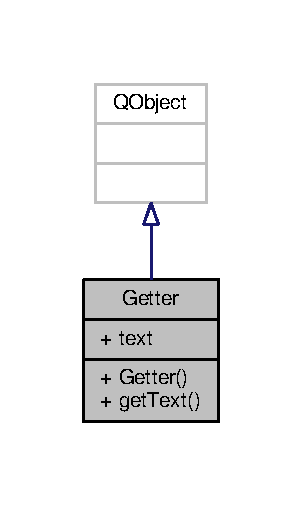
\includegraphics[width=145pt]{classGetter__inherit__graph}
\end{center}
\end{figure}


Collaboration diagram for Getter\+:
\nopagebreak
\begin{figure}[H]
\begin{center}
\leavevmode
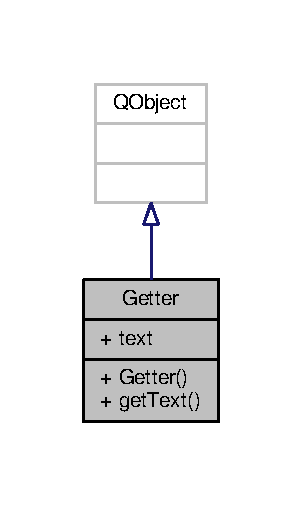
\includegraphics[width=145pt]{classGetter__coll__graph}
\end{center}
\end{figure}
\subsection*{Public Slots}
\begin{DoxyCompactItemize}
\item 
void \hyperlink{classGetter_a6938656fc1066da7f9d751add4bf2f73}{get\+Text} (Q\+String \+\_\+text)
\end{DoxyCompactItemize}
\subsection*{Public Member Functions}
\begin{DoxyCompactItemize}
\item 
\hyperlink{classGetter_afb7c0456242a77b2305fcbf4baf31087}{Getter} ()
\end{DoxyCompactItemize}
\subsection*{Public Attributes}
\begin{DoxyCompactItemize}
\item 
Q\+String \hyperlink{classGetter_a3ae6057d8e7030e28e74118b71cd07c0}{text}
\end{DoxyCompactItemize}


\subsection{Constructor \& Destructor Documentation}
\index{Getter@{Getter}!Getter@{Getter}}
\index{Getter@{Getter}!Getter@{Getter}}
\subsubsection[{\texorpdfstring{Getter()}{Getter()}}]{\setlength{\rightskip}{0pt plus 5cm}Getter\+::\+Getter (
\begin{DoxyParamCaption}
{}
\end{DoxyParamCaption}
)\hspace{0.3cm}{\ttfamily [inline]}}\hypertarget{classGetter_afb7c0456242a77b2305fcbf4baf31087}{}\label{classGetter_afb7c0456242a77b2305fcbf4baf31087}


\subsection{Member Function Documentation}
\index{Getter@{Getter}!get\+Text@{get\+Text}}
\index{get\+Text@{get\+Text}!Getter@{Getter}}
\subsubsection[{\texorpdfstring{get\+Text}{getText}}]{\setlength{\rightskip}{0pt plus 5cm}void Getter\+::get\+Text (
\begin{DoxyParamCaption}
\item[{Q\+String}]{\+\_\+text}
\end{DoxyParamCaption}
)\hspace{0.3cm}{\ttfamily [inline]}, {\ttfamily [slot]}}\hypertarget{classGetter_a6938656fc1066da7f9d751add4bf2f73}{}\label{classGetter_a6938656fc1066da7f9d751add4bf2f73}


\subsection{Member Data Documentation}
\index{Getter@{Getter}!text@{text}}
\index{text@{text}!Getter@{Getter}}
\subsubsection[{\texorpdfstring{text}{text}}]{\setlength{\rightskip}{0pt plus 5cm}Q\+String Getter\+::text}\hypertarget{classGetter_a3ae6057d8e7030e28e74118b71cd07c0}{}\label{classGetter_a3ae6057d8e7030e28e74118b71cd07c0}


The documentation for this class was generated from the following file\+:\begin{DoxyCompactItemize}
\item 
\hyperlink{ipinput_8h}{ipinput.\+h}\end{DoxyCompactItemize}

\hypertarget{classGomoku}{}\section{Gomoku Class Reference}
\label{classGomoku}\index{Gomoku@{Gomoku}}


Main window.  




{\ttfamily \#include $<$gomoku.\+h$>$}



Inheritance diagram for Gomoku\+:
\nopagebreak
\begin{figure}[H]
\begin{center}
\leavevmode
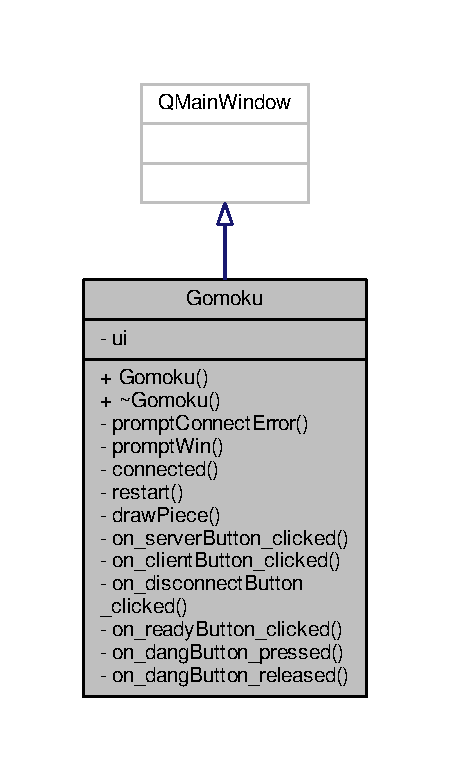
\includegraphics[width=216pt]{classGomoku__inherit__graph}
\end{center}
\end{figure}


Collaboration diagram for Gomoku\+:
\nopagebreak
\begin{figure}[H]
\begin{center}
\leavevmode
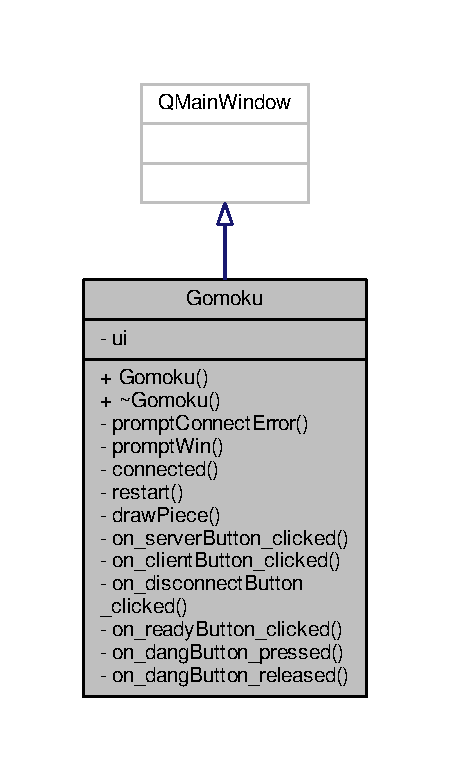
\includegraphics[width=216pt]{classGomoku__coll__graph}
\end{center}
\end{figure}
\subsection*{Public Member Functions}
\begin{DoxyCompactItemize}
\item 
\hyperlink{classGomoku_a15ad6f6d31efe9e4828ba79985d8880d}{Gomoku} (Q\+Widget $\ast$parent=0)
\item 
\hyperlink{classGomoku_a13a08a648094406111ba1b8b76047e37}{$\sim$\+Gomoku} ()
\end{DoxyCompactItemize}
\subsection*{Private Slots}
\begin{DoxyCompactItemize}
\item 
void \hyperlink{classGomoku_aafba38e2b2db2f0f0262a04b371b65b8}{prompt\+Connect\+Error} ()
\item 
void \hyperlink{classGomoku_a32aa94d4d8d3e340cd719e84ad51409d}{prompt\+Win} (bool color)
\item 
void \hyperlink{classGomoku_af7ab4e7e8061535ad746cb839f941fc6}{connected} ()
\item 
void \hyperlink{classGomoku_a9dde3f2dc64f4328918b0050e9635f98}{restart} ()
\begin{DoxyCompactList}\small\item\em clear board and reset color \end{DoxyCompactList}\item 
void \hyperlink{classGomoku_ada061f4b14409da12995cbe5e257e67e}{draw\+Piece} (int row, int column, bool color)
\item 
void \hyperlink{classGomoku_a763119d315fe24ef55bc581e67836856}{on\+\_\+server\+Button\+\_\+clicked} (bool checked)
\item 
void \hyperlink{classGomoku_a69e00fb73a572a157bd93e9720987c54}{on\+\_\+client\+Button\+\_\+clicked} (bool checked)
\item 
void \hyperlink{classGomoku_a8722500f524e6902a423ec33f31159a9}{on\+\_\+disconnect\+Button\+\_\+clicked} (bool checked)
\item 
void \hyperlink{classGomoku_a123db139238bd134421ae0cd7756bc84}{on\+\_\+ready\+Button\+\_\+clicked} (bool checked)
\item 
void \hyperlink{classGomoku_a0a1c400cb33e45b092931f99de732dd0}{on\+\_\+dang\+Button\+\_\+pressed} ()
\item 
void \hyperlink{classGomoku_aa703e7bc0d628d98f6f20a6f861e92d7}{on\+\_\+dang\+Button\+\_\+released} ()
\end{DoxyCompactItemize}
\subsection*{Private Attributes}
\begin{DoxyCompactItemize}
\item 
Ui\+::\+Gomoku $\ast$ \hyperlink{classGomoku_ac7bd58f9bde18d468518e5f78c458cf9}{ui}
\end{DoxyCompactItemize}


\subsection{Detailed Description}
Main window. 

\subsection{Constructor \& Destructor Documentation}
\index{Gomoku@{Gomoku}!Gomoku@{Gomoku}}
\index{Gomoku@{Gomoku}!Gomoku@{Gomoku}}
\subsubsection[{\texorpdfstring{Gomoku(\+Q\+Widget $\ast$parent=0)}{Gomoku(QWidget *parent=0)}}]{\setlength{\rightskip}{0pt plus 5cm}Gomoku\+::\+Gomoku (
\begin{DoxyParamCaption}
\item[{Q\+Widget $\ast$}]{parent = {\ttfamily 0}}
\end{DoxyParamCaption}
)\hspace{0.3cm}{\ttfamily [explicit]}}\hypertarget{classGomoku_a15ad6f6d31efe9e4828ba79985d8880d}{}\label{classGomoku_a15ad6f6d31efe9e4828ba79985d8880d}
\index{Gomoku@{Gomoku}!````~Gomoku@{$\sim$\+Gomoku}}
\index{````~Gomoku@{$\sim$\+Gomoku}!Gomoku@{Gomoku}}
\subsubsection[{\texorpdfstring{$\sim$\+Gomoku()}{~Gomoku()}}]{\setlength{\rightskip}{0pt plus 5cm}Gomoku\+::$\sim$\+Gomoku (
\begin{DoxyParamCaption}
{}
\end{DoxyParamCaption}
)}\hypertarget{classGomoku_a13a08a648094406111ba1b8b76047e37}{}\label{classGomoku_a13a08a648094406111ba1b8b76047e37}


\subsection{Member Function Documentation}
\index{Gomoku@{Gomoku}!connected@{connected}}
\index{connected@{connected}!Gomoku@{Gomoku}}
\subsubsection[{\texorpdfstring{connected}{connected}}]{\setlength{\rightskip}{0pt plus 5cm}void Gomoku\+::connected (
\begin{DoxyParamCaption}
{}
\end{DoxyParamCaption}
)\hspace{0.3cm}{\ttfamily [private]}, {\ttfamily [slot]}}\hypertarget{classGomoku_af7ab4e7e8061535ad746cb839f941fc6}{}\label{classGomoku_af7ab4e7e8061535ad746cb839f941fc6}
\index{Gomoku@{Gomoku}!draw\+Piece@{draw\+Piece}}
\index{draw\+Piece@{draw\+Piece}!Gomoku@{Gomoku}}
\subsubsection[{\texorpdfstring{draw\+Piece}{drawPiece}}]{\setlength{\rightskip}{0pt plus 5cm}void Gomoku\+::draw\+Piece (
\begin{DoxyParamCaption}
\item[{int}]{row, }
\item[{int}]{column, }
\item[{bool}]{color}
\end{DoxyParamCaption}
)\hspace{0.3cm}{\ttfamily [private]}, {\ttfamily [slot]}}\hypertarget{classGomoku_ada061f4b14409da12995cbe5e257e67e}{}\label{classGomoku_ada061f4b14409da12995cbe5e257e67e}
\index{Gomoku@{Gomoku}!on\+\_\+client\+Button\+\_\+clicked@{on\+\_\+client\+Button\+\_\+clicked}}
\index{on\+\_\+client\+Button\+\_\+clicked@{on\+\_\+client\+Button\+\_\+clicked}!Gomoku@{Gomoku}}
\subsubsection[{\texorpdfstring{on\+\_\+client\+Button\+\_\+clicked}{on_clientButton_clicked}}]{\setlength{\rightskip}{0pt plus 5cm}void Gomoku\+::on\+\_\+client\+Button\+\_\+clicked (
\begin{DoxyParamCaption}
\item[{bool}]{checked}
\end{DoxyParamCaption}
)\hspace{0.3cm}{\ttfamily [private]}, {\ttfamily [slot]}}\hypertarget{classGomoku_a69e00fb73a572a157bd93e9720987c54}{}\label{classGomoku_a69e00fb73a572a157bd93e9720987c54}
\index{Gomoku@{Gomoku}!on\+\_\+dang\+Button\+\_\+pressed@{on\+\_\+dang\+Button\+\_\+pressed}}
\index{on\+\_\+dang\+Button\+\_\+pressed@{on\+\_\+dang\+Button\+\_\+pressed}!Gomoku@{Gomoku}}
\subsubsection[{\texorpdfstring{on\+\_\+dang\+Button\+\_\+pressed}{on_dangButton_pressed}}]{\setlength{\rightskip}{0pt plus 5cm}void Gomoku\+::on\+\_\+dang\+Button\+\_\+pressed (
\begin{DoxyParamCaption}
{}
\end{DoxyParamCaption}
)\hspace{0.3cm}{\ttfamily [private]}, {\ttfamily [slot]}}\hypertarget{classGomoku_a0a1c400cb33e45b092931f99de732dd0}{}\label{classGomoku_a0a1c400cb33e45b092931f99de732dd0}
\index{Gomoku@{Gomoku}!on\+\_\+dang\+Button\+\_\+released@{on\+\_\+dang\+Button\+\_\+released}}
\index{on\+\_\+dang\+Button\+\_\+released@{on\+\_\+dang\+Button\+\_\+released}!Gomoku@{Gomoku}}
\subsubsection[{\texorpdfstring{on\+\_\+dang\+Button\+\_\+released}{on_dangButton_released}}]{\setlength{\rightskip}{0pt plus 5cm}void Gomoku\+::on\+\_\+dang\+Button\+\_\+released (
\begin{DoxyParamCaption}
{}
\end{DoxyParamCaption}
)\hspace{0.3cm}{\ttfamily [private]}, {\ttfamily [slot]}}\hypertarget{classGomoku_aa703e7bc0d628d98f6f20a6f861e92d7}{}\label{classGomoku_aa703e7bc0d628d98f6f20a6f861e92d7}
\index{Gomoku@{Gomoku}!on\+\_\+disconnect\+Button\+\_\+clicked@{on\+\_\+disconnect\+Button\+\_\+clicked}}
\index{on\+\_\+disconnect\+Button\+\_\+clicked@{on\+\_\+disconnect\+Button\+\_\+clicked}!Gomoku@{Gomoku}}
\subsubsection[{\texorpdfstring{on\+\_\+disconnect\+Button\+\_\+clicked}{on_disconnectButton_clicked}}]{\setlength{\rightskip}{0pt plus 5cm}void Gomoku\+::on\+\_\+disconnect\+Button\+\_\+clicked (
\begin{DoxyParamCaption}
\item[{bool}]{checked}
\end{DoxyParamCaption}
)\hspace{0.3cm}{\ttfamily [private]}, {\ttfamily [slot]}}\hypertarget{classGomoku_a8722500f524e6902a423ec33f31159a9}{}\label{classGomoku_a8722500f524e6902a423ec33f31159a9}
\index{Gomoku@{Gomoku}!on\+\_\+ready\+Button\+\_\+clicked@{on\+\_\+ready\+Button\+\_\+clicked}}
\index{on\+\_\+ready\+Button\+\_\+clicked@{on\+\_\+ready\+Button\+\_\+clicked}!Gomoku@{Gomoku}}
\subsubsection[{\texorpdfstring{on\+\_\+ready\+Button\+\_\+clicked}{on_readyButton_clicked}}]{\setlength{\rightskip}{0pt plus 5cm}void Gomoku\+::on\+\_\+ready\+Button\+\_\+clicked (
\begin{DoxyParamCaption}
\item[{bool}]{checked}
\end{DoxyParamCaption}
)\hspace{0.3cm}{\ttfamily [private]}, {\ttfamily [slot]}}\hypertarget{classGomoku_a123db139238bd134421ae0cd7756bc84}{}\label{classGomoku_a123db139238bd134421ae0cd7756bc84}
\index{Gomoku@{Gomoku}!on\+\_\+server\+Button\+\_\+clicked@{on\+\_\+server\+Button\+\_\+clicked}}
\index{on\+\_\+server\+Button\+\_\+clicked@{on\+\_\+server\+Button\+\_\+clicked}!Gomoku@{Gomoku}}
\subsubsection[{\texorpdfstring{on\+\_\+server\+Button\+\_\+clicked}{on_serverButton_clicked}}]{\setlength{\rightskip}{0pt plus 5cm}void Gomoku\+::on\+\_\+server\+Button\+\_\+clicked (
\begin{DoxyParamCaption}
\item[{bool}]{checked}
\end{DoxyParamCaption}
)\hspace{0.3cm}{\ttfamily [private]}, {\ttfamily [slot]}}\hypertarget{classGomoku_a763119d315fe24ef55bc581e67836856}{}\label{classGomoku_a763119d315fe24ef55bc581e67836856}
\index{Gomoku@{Gomoku}!prompt\+Connect\+Error@{prompt\+Connect\+Error}}
\index{prompt\+Connect\+Error@{prompt\+Connect\+Error}!Gomoku@{Gomoku}}
\subsubsection[{\texorpdfstring{prompt\+Connect\+Error}{promptConnectError}}]{\setlength{\rightskip}{0pt plus 5cm}void Gomoku\+::prompt\+Connect\+Error (
\begin{DoxyParamCaption}
{}
\end{DoxyParamCaption}
)\hspace{0.3cm}{\ttfamily [private]}, {\ttfamily [slot]}}\hypertarget{classGomoku_aafba38e2b2db2f0f0262a04b371b65b8}{}\label{classGomoku_aafba38e2b2db2f0f0262a04b371b65b8}
\index{Gomoku@{Gomoku}!prompt\+Win@{prompt\+Win}}
\index{prompt\+Win@{prompt\+Win}!Gomoku@{Gomoku}}
\subsubsection[{\texorpdfstring{prompt\+Win}{promptWin}}]{\setlength{\rightskip}{0pt plus 5cm}void Gomoku\+::prompt\+Win (
\begin{DoxyParamCaption}
\item[{bool}]{color}
\end{DoxyParamCaption}
)\hspace{0.3cm}{\ttfamily [private]}, {\ttfamily [slot]}}\hypertarget{classGomoku_a32aa94d4d8d3e340cd719e84ad51409d}{}\label{classGomoku_a32aa94d4d8d3e340cd719e84ad51409d}
\index{Gomoku@{Gomoku}!restart@{restart}}
\index{restart@{restart}!Gomoku@{Gomoku}}
\subsubsection[{\texorpdfstring{restart}{restart}}]{\setlength{\rightskip}{0pt plus 5cm}void Gomoku\+::restart (
\begin{DoxyParamCaption}
{}
\end{DoxyParamCaption}
)\hspace{0.3cm}{\ttfamily [private]}, {\ttfamily [slot]}}\hypertarget{classGomoku_a9dde3f2dc64f4328918b0050e9635f98}{}\label{classGomoku_a9dde3f2dc64f4328918b0050e9635f98}


clear board and reset color 



\subsection{Member Data Documentation}
\index{Gomoku@{Gomoku}!ui@{ui}}
\index{ui@{ui}!Gomoku@{Gomoku}}
\subsubsection[{\texorpdfstring{ui}{ui}}]{\setlength{\rightskip}{0pt plus 5cm}Ui\+::\+Gomoku$\ast$ Gomoku\+::ui\hspace{0.3cm}{\ttfamily [private]}}\hypertarget{classGomoku_ac7bd58f9bde18d468518e5f78c458cf9}{}\label{classGomoku_ac7bd58f9bde18d468518e5f78c458cf9}


The documentation for this class was generated from the following files\+:\begin{DoxyCompactItemize}
\item 
\hyperlink{gomoku_8h}{gomoku.\+h}\item 
\hyperlink{gomoku_8cpp}{gomoku.\+cpp}\end{DoxyCompactItemize}

\hypertarget{classInput}{}\section{Input Class Reference}
\label{classInput}\index{Input@{Input}}


Base class for user input from local or remote.  




{\ttfamily \#include $<$input.\+h$>$}



Inheritance diagram for Input\+:
\nopagebreak
\begin{figure}[H]
\begin{center}
\leavevmode
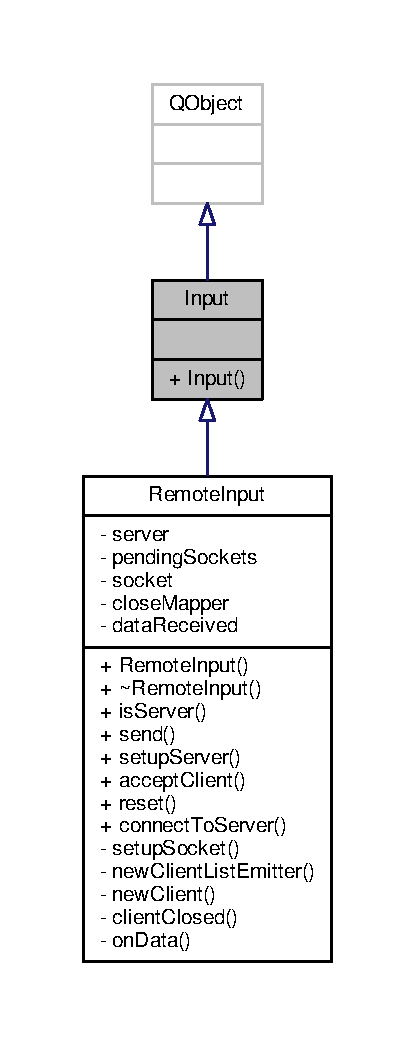
\includegraphics[width=199pt]{classInput__inherit__graph}
\end{center}
\end{figure}


Collaboration diagram for Input\+:
\nopagebreak
\begin{figure}[H]
\begin{center}
\leavevmode
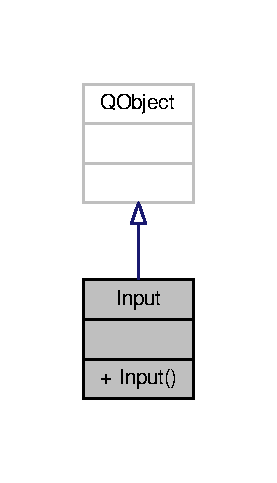
\includegraphics[width=133pt]{classInput__coll__graph}
\end{center}
\end{figure}
\subsection*{Signals}
\begin{DoxyCompactItemize}
\item 
void \hyperlink{classInput_a4871f3d5d214bf0bd39ce4b336b70d63}{draw} (int row, int column)
\begin{DoxyCompactList}\small\item\em draw a piece \end{DoxyCompactList}\end{DoxyCompactItemize}
\subsection*{Public Member Functions}
\begin{DoxyCompactItemize}
\item 
\hyperlink{classInput_a1e62cdfd419302414d2bf5de1d5fd1a7}{Input} (Q\+Object $\ast$parent)
\end{DoxyCompactItemize}


\subsection{Detailed Description}
Base class for user input from local or remote. 

\subsection{Constructor \& Destructor Documentation}
\index{Input@{Input}!Input@{Input}}
\index{Input@{Input}!Input@{Input}}
\subsubsection[{\texorpdfstring{Input(\+Q\+Object $\ast$parent)}{Input(QObject *parent)}}]{\setlength{\rightskip}{0pt plus 5cm}Input\+::\+Input (
\begin{DoxyParamCaption}
\item[{Q\+Object $\ast$}]{parent}
\end{DoxyParamCaption}
)\hspace{0.3cm}{\ttfamily [explicit]}}\hypertarget{classInput_a1e62cdfd419302414d2bf5de1d5fd1a7}{}\label{classInput_a1e62cdfd419302414d2bf5de1d5fd1a7}


\subsection{Member Function Documentation}
\index{Input@{Input}!draw@{draw}}
\index{draw@{draw}!Input@{Input}}
\subsubsection[{\texorpdfstring{draw}{draw}}]{\setlength{\rightskip}{0pt plus 5cm}void Input\+::draw (
\begin{DoxyParamCaption}
\item[{int}]{row, }
\item[{int}]{column}
\end{DoxyParamCaption}
)\hspace{0.3cm}{\ttfamily [signal]}}\hypertarget{classInput_a4871f3d5d214bf0bd39ce4b336b70d63}{}\label{classInput_a4871f3d5d214bf0bd39ce4b336b70d63}


draw a piece 



The documentation for this class was generated from the following files\+:\begin{DoxyCompactItemize}
\item 
\hyperlink{input_8h}{input.\+h}\item 
\hyperlink{input_8cpp}{input.\+cpp}\end{DoxyCompactItemize}

\hypertarget{classIpInput}{}\section{Ip\+Input Class Reference}
\label{classIpInput}\index{Ip\+Input@{Ip\+Input}}


{\ttfamily \#include $<$ipinput.\+h$>$}



Inheritance diagram for Ip\+Input\+:
\nopagebreak
\begin{figure}[H]
\begin{center}
\leavevmode
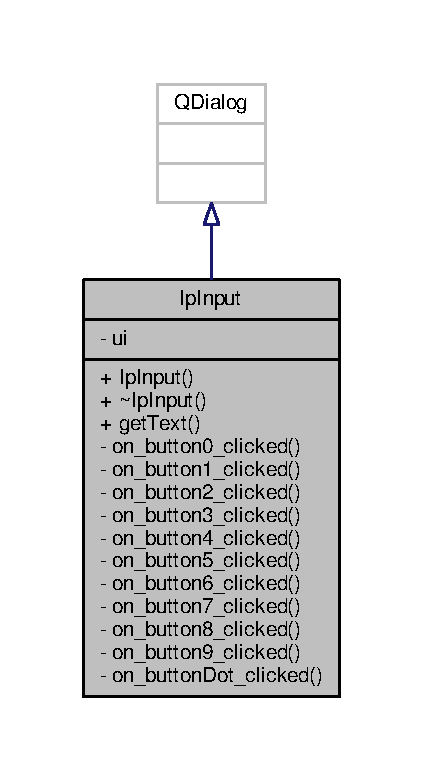
\includegraphics[width=203pt]{classIpInput__inherit__graph}
\end{center}
\end{figure}


Collaboration diagram for Ip\+Input\+:
\nopagebreak
\begin{figure}[H]
\begin{center}
\leavevmode
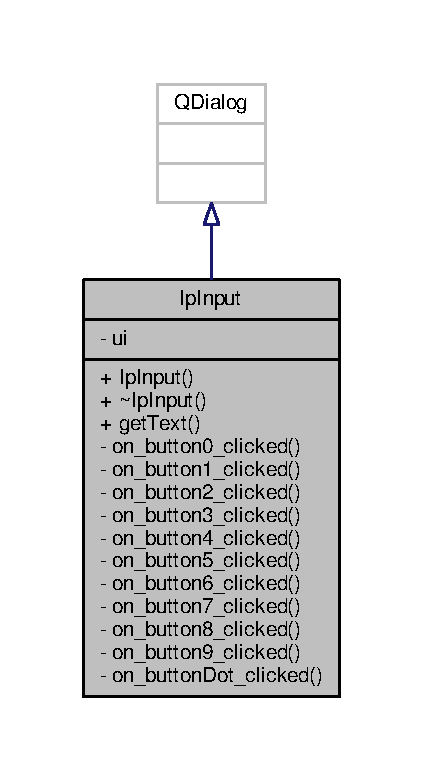
\includegraphics[width=203pt]{classIpInput__coll__graph}
\end{center}
\end{figure}
\subsection*{Public Member Functions}
\begin{DoxyCompactItemize}
\item 
\hyperlink{classIpInput_aed9e4a942a9ffd744b05c40e5fb3d506}{Ip\+Input} (Q\+Widget $\ast$parent=0)
\item 
\hyperlink{classIpInput_ab194007adfec0b4c8ed44e3f6531ac44}{$\sim$\+Ip\+Input} ()
\end{DoxyCompactItemize}
\subsection*{Static Public Member Functions}
\begin{DoxyCompactItemize}
\item 
static Q\+String \hyperlink{classIpInput_a4cf4786bfd38290ffb42399eefc11815}{get\+Text} ()
\end{DoxyCompactItemize}
\subsection*{Private Slots}
\begin{DoxyCompactItemize}
\item 
void \hyperlink{classIpInput_a1fc1ff2a2b0e350bbcc6e3e72ec7f044}{on\+\_\+button0\+\_\+clicked} (bool checked)
\item 
void \hyperlink{classIpInput_a451d6827bc280d34146d9cd843f660c8}{on\+\_\+button1\+\_\+clicked} (bool checked)
\item 
void \hyperlink{classIpInput_ac07b5e8c83bcba986956178758517963}{on\+\_\+button2\+\_\+clicked} (bool checked)
\item 
void \hyperlink{classIpInput_a88b3d07330a41ce3d2e6e66cbc1591c5}{on\+\_\+button3\+\_\+clicked} (bool checked)
\item 
void \hyperlink{classIpInput_abc78ea1e2349a87dca700beb11edc74f}{on\+\_\+button4\+\_\+clicked} (bool checked)
\item 
void \hyperlink{classIpInput_a1506bb196e4ed1bf7432e37c3a7fa180}{on\+\_\+button5\+\_\+clicked} (bool checked)
\item 
void \hyperlink{classIpInput_ade74543fea80105b34daffb61c956fc2}{on\+\_\+button6\+\_\+clicked} (bool checked)
\item 
void \hyperlink{classIpInput_a77cdc98b7572afa030e58f637e05e7de}{on\+\_\+button7\+\_\+clicked} (bool checked)
\item 
void \hyperlink{classIpInput_a994482d6c14304778f38276dbe6ce8a8}{on\+\_\+button8\+\_\+clicked} (bool checked)
\item 
void \hyperlink{classIpInput_ab3bb6c47e2a7b30e05462be39623fbd9}{on\+\_\+button9\+\_\+clicked} (bool checked)
\item 
void \hyperlink{classIpInput_add23563d5448f2c8240b06347676c649}{on\+\_\+button\+Dot\+\_\+clicked} (bool checked)
\end{DoxyCompactItemize}
\subsection*{Private Attributes}
\begin{DoxyCompactItemize}
\item 
Ui\+::\+Ip\+Input $\ast$ \hyperlink{classIpInput_a867b68834adba8912e05242487a6eb13}{ui}
\end{DoxyCompactItemize}


\subsection{Constructor \& Destructor Documentation}
\index{Ip\+Input@{Ip\+Input}!Ip\+Input@{Ip\+Input}}
\index{Ip\+Input@{Ip\+Input}!Ip\+Input@{Ip\+Input}}
\subsubsection[{\texorpdfstring{Ip\+Input(\+Q\+Widget $\ast$parent=0)}{IpInput(QWidget *parent=0)}}]{\setlength{\rightskip}{0pt plus 5cm}Ip\+Input\+::\+Ip\+Input (
\begin{DoxyParamCaption}
\item[{Q\+Widget $\ast$}]{parent = {\ttfamily 0}}
\end{DoxyParamCaption}
)\hspace{0.3cm}{\ttfamily [explicit]}}\hypertarget{classIpInput_aed9e4a942a9ffd744b05c40e5fb3d506}{}\label{classIpInput_aed9e4a942a9ffd744b05c40e5fb3d506}
\index{Ip\+Input@{Ip\+Input}!````~Ip\+Input@{$\sim$\+Ip\+Input}}
\index{````~Ip\+Input@{$\sim$\+Ip\+Input}!Ip\+Input@{Ip\+Input}}
\subsubsection[{\texorpdfstring{$\sim$\+Ip\+Input()}{~IpInput()}}]{\setlength{\rightskip}{0pt plus 5cm}Ip\+Input\+::$\sim$\+Ip\+Input (
\begin{DoxyParamCaption}
{}
\end{DoxyParamCaption}
)}\hypertarget{classIpInput_ab194007adfec0b4c8ed44e3f6531ac44}{}\label{classIpInput_ab194007adfec0b4c8ed44e3f6531ac44}


\subsection{Member Function Documentation}
\index{Ip\+Input@{Ip\+Input}!get\+Text@{get\+Text}}
\index{get\+Text@{get\+Text}!Ip\+Input@{Ip\+Input}}
\subsubsection[{\texorpdfstring{get\+Text()}{getText()}}]{\setlength{\rightskip}{0pt plus 5cm}Q\+String Ip\+Input\+::get\+Text (
\begin{DoxyParamCaption}
{}
\end{DoxyParamCaption}
)\hspace{0.3cm}{\ttfamily [static]}}\hypertarget{classIpInput_a4cf4786bfd38290ffb42399eefc11815}{}\label{classIpInput_a4cf4786bfd38290ffb42399eefc11815}
\index{Ip\+Input@{Ip\+Input}!on\+\_\+button0\+\_\+clicked@{on\+\_\+button0\+\_\+clicked}}
\index{on\+\_\+button0\+\_\+clicked@{on\+\_\+button0\+\_\+clicked}!Ip\+Input@{Ip\+Input}}
\subsubsection[{\texorpdfstring{on\+\_\+button0\+\_\+clicked}{on_button0_clicked}}]{\setlength{\rightskip}{0pt plus 5cm}void Ip\+Input\+::on\+\_\+button0\+\_\+clicked (
\begin{DoxyParamCaption}
\item[{bool}]{checked}
\end{DoxyParamCaption}
)\hspace{0.3cm}{\ttfamily [private]}, {\ttfamily [slot]}}\hypertarget{classIpInput_a1fc1ff2a2b0e350bbcc6e3e72ec7f044}{}\label{classIpInput_a1fc1ff2a2b0e350bbcc6e3e72ec7f044}
\index{Ip\+Input@{Ip\+Input}!on\+\_\+button1\+\_\+clicked@{on\+\_\+button1\+\_\+clicked}}
\index{on\+\_\+button1\+\_\+clicked@{on\+\_\+button1\+\_\+clicked}!Ip\+Input@{Ip\+Input}}
\subsubsection[{\texorpdfstring{on\+\_\+button1\+\_\+clicked}{on_button1_clicked}}]{\setlength{\rightskip}{0pt plus 5cm}void Ip\+Input\+::on\+\_\+button1\+\_\+clicked (
\begin{DoxyParamCaption}
\item[{bool}]{checked}
\end{DoxyParamCaption}
)\hspace{0.3cm}{\ttfamily [private]}, {\ttfamily [slot]}}\hypertarget{classIpInput_a451d6827bc280d34146d9cd843f660c8}{}\label{classIpInput_a451d6827bc280d34146d9cd843f660c8}
\index{Ip\+Input@{Ip\+Input}!on\+\_\+button2\+\_\+clicked@{on\+\_\+button2\+\_\+clicked}}
\index{on\+\_\+button2\+\_\+clicked@{on\+\_\+button2\+\_\+clicked}!Ip\+Input@{Ip\+Input}}
\subsubsection[{\texorpdfstring{on\+\_\+button2\+\_\+clicked}{on_button2_clicked}}]{\setlength{\rightskip}{0pt plus 5cm}void Ip\+Input\+::on\+\_\+button2\+\_\+clicked (
\begin{DoxyParamCaption}
\item[{bool}]{checked}
\end{DoxyParamCaption}
)\hspace{0.3cm}{\ttfamily [private]}, {\ttfamily [slot]}}\hypertarget{classIpInput_ac07b5e8c83bcba986956178758517963}{}\label{classIpInput_ac07b5e8c83bcba986956178758517963}
\index{Ip\+Input@{Ip\+Input}!on\+\_\+button3\+\_\+clicked@{on\+\_\+button3\+\_\+clicked}}
\index{on\+\_\+button3\+\_\+clicked@{on\+\_\+button3\+\_\+clicked}!Ip\+Input@{Ip\+Input}}
\subsubsection[{\texorpdfstring{on\+\_\+button3\+\_\+clicked}{on_button3_clicked}}]{\setlength{\rightskip}{0pt plus 5cm}void Ip\+Input\+::on\+\_\+button3\+\_\+clicked (
\begin{DoxyParamCaption}
\item[{bool}]{checked}
\end{DoxyParamCaption}
)\hspace{0.3cm}{\ttfamily [private]}, {\ttfamily [slot]}}\hypertarget{classIpInput_a88b3d07330a41ce3d2e6e66cbc1591c5}{}\label{classIpInput_a88b3d07330a41ce3d2e6e66cbc1591c5}
\index{Ip\+Input@{Ip\+Input}!on\+\_\+button4\+\_\+clicked@{on\+\_\+button4\+\_\+clicked}}
\index{on\+\_\+button4\+\_\+clicked@{on\+\_\+button4\+\_\+clicked}!Ip\+Input@{Ip\+Input}}
\subsubsection[{\texorpdfstring{on\+\_\+button4\+\_\+clicked}{on_button4_clicked}}]{\setlength{\rightskip}{0pt plus 5cm}void Ip\+Input\+::on\+\_\+button4\+\_\+clicked (
\begin{DoxyParamCaption}
\item[{bool}]{checked}
\end{DoxyParamCaption}
)\hspace{0.3cm}{\ttfamily [private]}, {\ttfamily [slot]}}\hypertarget{classIpInput_abc78ea1e2349a87dca700beb11edc74f}{}\label{classIpInput_abc78ea1e2349a87dca700beb11edc74f}
\index{Ip\+Input@{Ip\+Input}!on\+\_\+button5\+\_\+clicked@{on\+\_\+button5\+\_\+clicked}}
\index{on\+\_\+button5\+\_\+clicked@{on\+\_\+button5\+\_\+clicked}!Ip\+Input@{Ip\+Input}}
\subsubsection[{\texorpdfstring{on\+\_\+button5\+\_\+clicked}{on_button5_clicked}}]{\setlength{\rightskip}{0pt plus 5cm}void Ip\+Input\+::on\+\_\+button5\+\_\+clicked (
\begin{DoxyParamCaption}
\item[{bool}]{checked}
\end{DoxyParamCaption}
)\hspace{0.3cm}{\ttfamily [private]}, {\ttfamily [slot]}}\hypertarget{classIpInput_a1506bb196e4ed1bf7432e37c3a7fa180}{}\label{classIpInput_a1506bb196e4ed1bf7432e37c3a7fa180}
\index{Ip\+Input@{Ip\+Input}!on\+\_\+button6\+\_\+clicked@{on\+\_\+button6\+\_\+clicked}}
\index{on\+\_\+button6\+\_\+clicked@{on\+\_\+button6\+\_\+clicked}!Ip\+Input@{Ip\+Input}}
\subsubsection[{\texorpdfstring{on\+\_\+button6\+\_\+clicked}{on_button6_clicked}}]{\setlength{\rightskip}{0pt plus 5cm}void Ip\+Input\+::on\+\_\+button6\+\_\+clicked (
\begin{DoxyParamCaption}
\item[{bool}]{checked}
\end{DoxyParamCaption}
)\hspace{0.3cm}{\ttfamily [private]}, {\ttfamily [slot]}}\hypertarget{classIpInput_ade74543fea80105b34daffb61c956fc2}{}\label{classIpInput_ade74543fea80105b34daffb61c956fc2}
\index{Ip\+Input@{Ip\+Input}!on\+\_\+button7\+\_\+clicked@{on\+\_\+button7\+\_\+clicked}}
\index{on\+\_\+button7\+\_\+clicked@{on\+\_\+button7\+\_\+clicked}!Ip\+Input@{Ip\+Input}}
\subsubsection[{\texorpdfstring{on\+\_\+button7\+\_\+clicked}{on_button7_clicked}}]{\setlength{\rightskip}{0pt plus 5cm}void Ip\+Input\+::on\+\_\+button7\+\_\+clicked (
\begin{DoxyParamCaption}
\item[{bool}]{checked}
\end{DoxyParamCaption}
)\hspace{0.3cm}{\ttfamily [private]}, {\ttfamily [slot]}}\hypertarget{classIpInput_a77cdc98b7572afa030e58f637e05e7de}{}\label{classIpInput_a77cdc98b7572afa030e58f637e05e7de}
\index{Ip\+Input@{Ip\+Input}!on\+\_\+button8\+\_\+clicked@{on\+\_\+button8\+\_\+clicked}}
\index{on\+\_\+button8\+\_\+clicked@{on\+\_\+button8\+\_\+clicked}!Ip\+Input@{Ip\+Input}}
\subsubsection[{\texorpdfstring{on\+\_\+button8\+\_\+clicked}{on_button8_clicked}}]{\setlength{\rightskip}{0pt plus 5cm}void Ip\+Input\+::on\+\_\+button8\+\_\+clicked (
\begin{DoxyParamCaption}
\item[{bool}]{checked}
\end{DoxyParamCaption}
)\hspace{0.3cm}{\ttfamily [private]}, {\ttfamily [slot]}}\hypertarget{classIpInput_a994482d6c14304778f38276dbe6ce8a8}{}\label{classIpInput_a994482d6c14304778f38276dbe6ce8a8}
\index{Ip\+Input@{Ip\+Input}!on\+\_\+button9\+\_\+clicked@{on\+\_\+button9\+\_\+clicked}}
\index{on\+\_\+button9\+\_\+clicked@{on\+\_\+button9\+\_\+clicked}!Ip\+Input@{Ip\+Input}}
\subsubsection[{\texorpdfstring{on\+\_\+button9\+\_\+clicked}{on_button9_clicked}}]{\setlength{\rightskip}{0pt plus 5cm}void Ip\+Input\+::on\+\_\+button9\+\_\+clicked (
\begin{DoxyParamCaption}
\item[{bool}]{checked}
\end{DoxyParamCaption}
)\hspace{0.3cm}{\ttfamily [private]}, {\ttfamily [slot]}}\hypertarget{classIpInput_ab3bb6c47e2a7b30e05462be39623fbd9}{}\label{classIpInput_ab3bb6c47e2a7b30e05462be39623fbd9}
\index{Ip\+Input@{Ip\+Input}!on\+\_\+button\+Dot\+\_\+clicked@{on\+\_\+button\+Dot\+\_\+clicked}}
\index{on\+\_\+button\+Dot\+\_\+clicked@{on\+\_\+button\+Dot\+\_\+clicked}!Ip\+Input@{Ip\+Input}}
\subsubsection[{\texorpdfstring{on\+\_\+button\+Dot\+\_\+clicked}{on_buttonDot_clicked}}]{\setlength{\rightskip}{0pt plus 5cm}void Ip\+Input\+::on\+\_\+button\+Dot\+\_\+clicked (
\begin{DoxyParamCaption}
\item[{bool}]{checked}
\end{DoxyParamCaption}
)\hspace{0.3cm}{\ttfamily [private]}, {\ttfamily [slot]}}\hypertarget{classIpInput_add23563d5448f2c8240b06347676c649}{}\label{classIpInput_add23563d5448f2c8240b06347676c649}


\subsection{Member Data Documentation}
\index{Ip\+Input@{Ip\+Input}!ui@{ui}}
\index{ui@{ui}!Ip\+Input@{Ip\+Input}}
\subsubsection[{\texorpdfstring{ui}{ui}}]{\setlength{\rightskip}{0pt plus 5cm}Ui\+::\+Ip\+Input$\ast$ Ip\+Input\+::ui\hspace{0.3cm}{\ttfamily [private]}}\hypertarget{classIpInput_a867b68834adba8912e05242487a6eb13}{}\label{classIpInput_a867b68834adba8912e05242487a6eb13}


The documentation for this class was generated from the following files\+:\begin{DoxyCompactItemize}
\item 
\hyperlink{ipinput_8h}{ipinput.\+h}\item 
\hyperlink{ipinput_8cpp}{ipinput.\+cpp}\end{DoxyCompactItemize}

\hypertarget{classRemoteInput}{}\section{Remote\+Input Class Reference}
\label{classRemoteInput}\index{Remote\+Input@{Remote\+Input}}


User input from remote.  




{\ttfamily \#include $<$remoteinput.\+h$>$}



Inheritance diagram for Remote\+Input\+:
\nopagebreak
\begin{figure}[H]
\begin{center}
\leavevmode
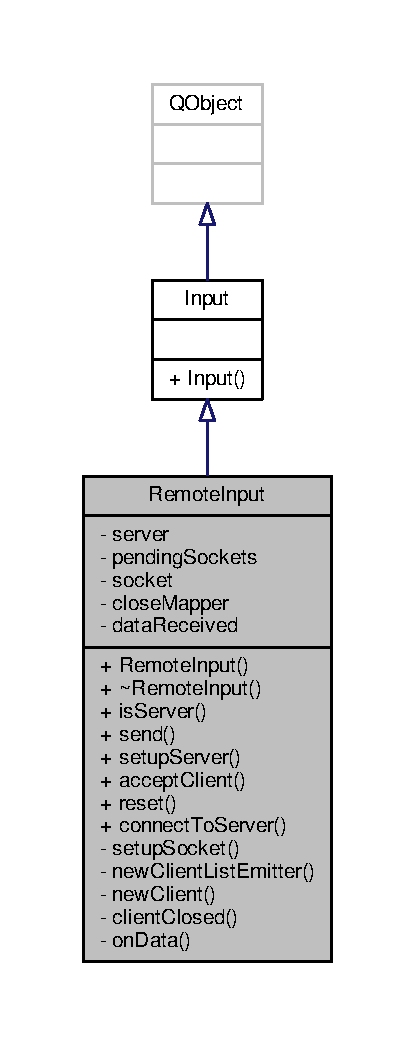
\includegraphics[width=199pt]{classRemoteInput__inherit__graph}
\end{center}
\end{figure}


Collaboration diagram for Remote\+Input\+:
\nopagebreak
\begin{figure}[H]
\begin{center}
\leavevmode
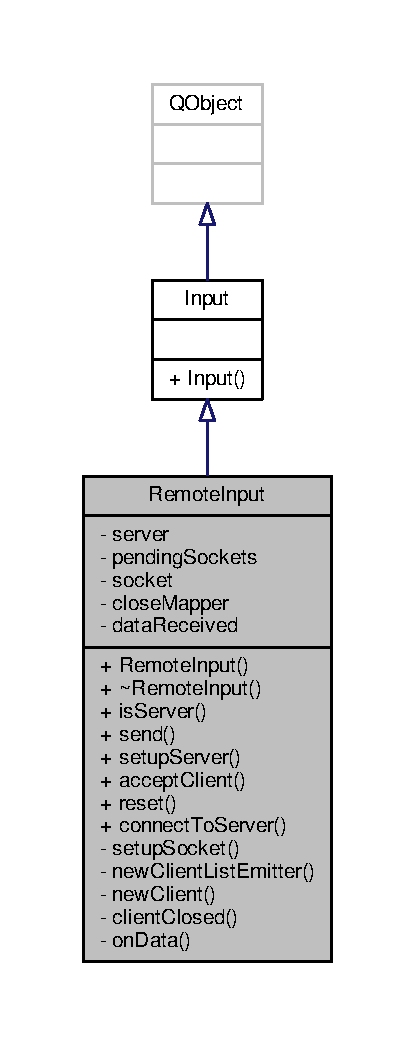
\includegraphics[width=199pt]{classRemoteInput__coll__graph}
\end{center}
\end{figure}
\subsection*{Public Slots}
\begin{DoxyCompactItemize}
\item 
void \hyperlink{classRemoteInput_a433cbb8d886d2c4b8dd61afcc40ee237}{setup\+Server} (const Q\+String \&addr)
\begin{DoxyCompactList}\small\item\em setup a server listening to {\ttfamily addr} \end{DoxyCompactList}\item 
void \hyperlink{classRemoteInput_ac7b675466378716bf4b60481dac71777}{accept\+Client} (int index)
\begin{DoxyCompactList}\small\item\em accept a client to be working socket {\ttfamily socket} \end{DoxyCompactList}\item 
void \hyperlink{classRemoteInput_ac7268f7b0c862ae1d45e7c85ed40b975}{reset} ()
\begin{DoxyCompactList}\small\item\em delete server and socket \end{DoxyCompactList}\item 
void \hyperlink{classRemoteInput_a59e3292c1516aa98ffe4ba6f6a318379}{connect\+To\+Server} (const Q\+String \&addr)
\begin{DoxyCompactList}\small\item\em connect to server \end{DoxyCompactList}\end{DoxyCompactItemize}
\subsection*{Signals}
\begin{DoxyCompactItemize}
\item 
void \hyperlink{classRemoteInput_a03854b31b3bd34a0c6714e34ea97fa51}{new\+Client\+List} (const Q\+List$<$ Q\+String $>$ \&list)
\begin{DoxyCompactList}\small\item\em emitted when client list changed \end{DoxyCompactList}\item 
void \hyperlink{classRemoteInput_a220a9df96569060dbaa459e4260ba5ac}{server\+Error} ()
\begin{DoxyCompactList}\small\item\em emitted when unable to setup server \end{DoxyCompactList}\item 
void \hyperlink{classRemoteInput_ace137f88c2ecb10d206282be259be88b}{connect\+Error} ()
\begin{DoxyCompactList}\small\item\em emitted when connection fails \end{DoxyCompactList}\item 
void \hyperlink{classRemoteInput_addd302fec13370bfc6818d5915844973}{hello} ()
\begin{DoxyCompactList}\small\item\em emitted when connection accepted by both side \end{DoxyCompactList}\item 
void \hyperlink{classRemoteInput_a9e8cb56fd11439e6bc12dd369d7ec4d1}{request\+Restart} ()
\begin{DoxyCompactList}\small\item\em emitted when the other user request restart \end{DoxyCompactList}\end{DoxyCompactItemize}
\subsection*{Public Member Functions}
\begin{DoxyCompactItemize}
\item 
\hyperlink{classRemoteInput_a7d80d0cdef9461614408a40dcc86536d}{Remote\+Input} (Q\+Object $\ast$parent)
\item 
\hyperlink{classRemoteInput_afa5a81b65b2cb9063263094492bbfcb0}{$\sim$\+Remote\+Input} ()
\item 
bool \hyperlink{classRemoteInput_ad4282349a4e2f17e277a5cde678fd295}{is\+Server} ()
\item 
void \hyperlink{classRemoteInput_aef618974f5cad6637ddce434dae2bcf2}{send} (const Q\+String \&method, const Q\+Json\+Object \&params=Q\+Json\+Object())
\begin{DoxyCompactList}\small\item\em Call remote method in J\+S\+ON format. \end{DoxyCompactList}\end{DoxyCompactItemize}
\subsection*{Private Slots}
\begin{DoxyCompactItemize}
\item 
void \hyperlink{classRemoteInput_a9185f78a38ff6504229604c90236d78b}{new\+Client} ()
\item 
void \hyperlink{classRemoteInput_a8d09dd6f3f7cd07bfd09a31c2ed47856}{client\+Closed} (Q\+Object $\ast$\+\_\+socket)
\item 
void \hyperlink{classRemoteInput_ae7ae71e93d5630bf16b2e624046d7560}{on\+Data} ()
\begin{DoxyCompactList}\small\item\em When data blocks received. \end{DoxyCompactList}\end{DoxyCompactItemize}
\subsection*{Private Member Functions}
\begin{DoxyCompactItemize}
\item 
void \hyperlink{classRemoteInput_a102e5869f429f046065582a281854f73}{setup\+Socket} ()
\item 
void \hyperlink{classRemoteInput_a31ec7cb4bea4187c5ad13ef4293c3904}{new\+Client\+List\+Emitter} ()
\end{DoxyCompactItemize}
\subsection*{Private Attributes}
\begin{DoxyCompactItemize}
\item 
Q\+Pointer$<$ Q\+Tcp\+Server $>$ \hyperlink{classRemoteInput_a85fb06e7f927436c6fe959935afa4185}{server}
\item 
Q\+List$<$ Q\+Pointer$<$ Q\+Tcp\+Socket $>$ $>$ \hyperlink{classRemoteInput_a8efa826116b9bed6bce016c4f6aedced}{pending\+Sockets}
\item 
Q\+Pointer$<$ Q\+Tcp\+Socket $>$ \hyperlink{classRemoteInput_a4d02f25eaa512b9dc5459d8296f1d11c}{socket}
\begin{DoxyCompactList}\small\item\em The socket that is working, no longer as server or client. \end{DoxyCompactList}\item 
Q\+Signal\+Mapper $\ast$ \hyperlink{classRemoteInput_a58e7c3fa294e6489d82be7c0aad27fdb}{close\+Mapper}
\begin{DoxyCompactList}\small\item\em transfer disconnection signal \end{DoxyCompactList}\item 
Q\+Byte\+Array \hyperlink{classRemoteInput_a32118b1d5726b5435b43b4a80e2b2532}{data\+Received}
\end{DoxyCompactItemize}


\subsection{Detailed Description}
User input from remote. 

\subsection{Constructor \& Destructor Documentation}
\index{Remote\+Input@{Remote\+Input}!Remote\+Input@{Remote\+Input}}
\index{Remote\+Input@{Remote\+Input}!Remote\+Input@{Remote\+Input}}
\subsubsection[{\texorpdfstring{Remote\+Input(\+Q\+Object $\ast$parent)}{RemoteInput(QObject *parent)}}]{\setlength{\rightskip}{0pt plus 5cm}Remote\+Input\+::\+Remote\+Input (
\begin{DoxyParamCaption}
\item[{Q\+Object $\ast$}]{parent}
\end{DoxyParamCaption}
)\hspace{0.3cm}{\ttfamily [explicit]}}\hypertarget{classRemoteInput_a7d80d0cdef9461614408a40dcc86536d}{}\label{classRemoteInput_a7d80d0cdef9461614408a40dcc86536d}
\index{Remote\+Input@{Remote\+Input}!````~Remote\+Input@{$\sim$\+Remote\+Input}}
\index{````~Remote\+Input@{$\sim$\+Remote\+Input}!Remote\+Input@{Remote\+Input}}
\subsubsection[{\texorpdfstring{$\sim$\+Remote\+Input()}{~RemoteInput()}}]{\setlength{\rightskip}{0pt plus 5cm}Remote\+Input\+::$\sim$\+Remote\+Input (
\begin{DoxyParamCaption}
{}
\end{DoxyParamCaption}
)}\hypertarget{classRemoteInput_afa5a81b65b2cb9063263094492bbfcb0}{}\label{classRemoteInput_afa5a81b65b2cb9063263094492bbfcb0}


\subsection{Member Function Documentation}
\index{Remote\+Input@{Remote\+Input}!accept\+Client@{accept\+Client}}
\index{accept\+Client@{accept\+Client}!Remote\+Input@{Remote\+Input}}
\subsubsection[{\texorpdfstring{accept\+Client}{acceptClient}}]{\setlength{\rightskip}{0pt plus 5cm}void Remote\+Input\+::accept\+Client (
\begin{DoxyParamCaption}
\item[{int}]{index}
\end{DoxyParamCaption}
)\hspace{0.3cm}{\ttfamily [slot]}}\hypertarget{classRemoteInput_ac7b675466378716bf4b60481dac71777}{}\label{classRemoteInput_ac7b675466378716bf4b60481dac71777}


accept a client to be working socket {\ttfamily socket} 

\index{Remote\+Input@{Remote\+Input}!client\+Closed@{client\+Closed}}
\index{client\+Closed@{client\+Closed}!Remote\+Input@{Remote\+Input}}
\subsubsection[{\texorpdfstring{client\+Closed}{clientClosed}}]{\setlength{\rightskip}{0pt plus 5cm}void Remote\+Input\+::client\+Closed (
\begin{DoxyParamCaption}
\item[{Q\+Object $\ast$}]{\+\_\+socket}
\end{DoxyParamCaption}
)\hspace{0.3cm}{\ttfamily [private]}, {\ttfamily [slot]}}\hypertarget{classRemoteInput_a8d09dd6f3f7cd07bfd09a31c2ed47856}{}\label{classRemoteInput_a8d09dd6f3f7cd07bfd09a31c2ed47856}
\index{Remote\+Input@{Remote\+Input}!connect\+Error@{connect\+Error}}
\index{connect\+Error@{connect\+Error}!Remote\+Input@{Remote\+Input}}
\subsubsection[{\texorpdfstring{connect\+Error}{connectError}}]{\setlength{\rightskip}{0pt plus 5cm}void Remote\+Input\+::connect\+Error (
\begin{DoxyParamCaption}
{}
\end{DoxyParamCaption}
)\hspace{0.3cm}{\ttfamily [signal]}}\hypertarget{classRemoteInput_ace137f88c2ecb10d206282be259be88b}{}\label{classRemoteInput_ace137f88c2ecb10d206282be259be88b}


emitted when connection fails 

\index{Remote\+Input@{Remote\+Input}!connect\+To\+Server@{connect\+To\+Server}}
\index{connect\+To\+Server@{connect\+To\+Server}!Remote\+Input@{Remote\+Input}}
\subsubsection[{\texorpdfstring{connect\+To\+Server}{connectToServer}}]{\setlength{\rightskip}{0pt plus 5cm}void Remote\+Input\+::connect\+To\+Server (
\begin{DoxyParamCaption}
\item[{const Q\+String \&}]{addr}
\end{DoxyParamCaption}
)\hspace{0.3cm}{\ttfamily [slot]}}\hypertarget{classRemoteInput_a59e3292c1516aa98ffe4ba6f6a318379}{}\label{classRemoteInput_a59e3292c1516aa98ffe4ba6f6a318379}


connect to server 

\index{Remote\+Input@{Remote\+Input}!hello@{hello}}
\index{hello@{hello}!Remote\+Input@{Remote\+Input}}
\subsubsection[{\texorpdfstring{hello}{hello}}]{\setlength{\rightskip}{0pt plus 5cm}void Remote\+Input\+::hello (
\begin{DoxyParamCaption}
{}
\end{DoxyParamCaption}
)\hspace{0.3cm}{\ttfamily [signal]}}\hypertarget{classRemoteInput_addd302fec13370bfc6818d5915844973}{}\label{classRemoteInput_addd302fec13370bfc6818d5915844973}


emitted when connection accepted by both side 

\index{Remote\+Input@{Remote\+Input}!is\+Server@{is\+Server}}
\index{is\+Server@{is\+Server}!Remote\+Input@{Remote\+Input}}
\subsubsection[{\texorpdfstring{is\+Server()}{isServer()}}]{\setlength{\rightskip}{0pt plus 5cm}bool Remote\+Input\+::is\+Server (
\begin{DoxyParamCaption}
{}
\end{DoxyParamCaption}
)\hspace{0.3cm}{\ttfamily [inline]}}\hypertarget{classRemoteInput_ad4282349a4e2f17e277a5cde678fd295}{}\label{classRemoteInput_ad4282349a4e2f17e277a5cde678fd295}
\index{Remote\+Input@{Remote\+Input}!new\+Client@{new\+Client}}
\index{new\+Client@{new\+Client}!Remote\+Input@{Remote\+Input}}
\subsubsection[{\texorpdfstring{new\+Client}{newClient}}]{\setlength{\rightskip}{0pt plus 5cm}void Remote\+Input\+::new\+Client (
\begin{DoxyParamCaption}
{}
\end{DoxyParamCaption}
)\hspace{0.3cm}{\ttfamily [private]}, {\ttfamily [slot]}}\hypertarget{classRemoteInput_a9185f78a38ff6504229604c90236d78b}{}\label{classRemoteInput_a9185f78a38ff6504229604c90236d78b}
\index{Remote\+Input@{Remote\+Input}!new\+Client\+List@{new\+Client\+List}}
\index{new\+Client\+List@{new\+Client\+List}!Remote\+Input@{Remote\+Input}}
\subsubsection[{\texorpdfstring{new\+Client\+List}{newClientList}}]{\setlength{\rightskip}{0pt plus 5cm}void Remote\+Input\+::new\+Client\+List (
\begin{DoxyParamCaption}
\item[{const Q\+List$<$ Q\+String $>$ \&}]{list}
\end{DoxyParamCaption}
)\hspace{0.3cm}{\ttfamily [signal]}}\hypertarget{classRemoteInput_a03854b31b3bd34a0c6714e34ea97fa51}{}\label{classRemoteInput_a03854b31b3bd34a0c6714e34ea97fa51}


emitted when client list changed 


\begin{DoxyParams}{Parameters}
{\em list} & of ips of clients \\
\hline
\end{DoxyParams}
\index{Remote\+Input@{Remote\+Input}!new\+Client\+List\+Emitter@{new\+Client\+List\+Emitter}}
\index{new\+Client\+List\+Emitter@{new\+Client\+List\+Emitter}!Remote\+Input@{Remote\+Input}}
\subsubsection[{\texorpdfstring{new\+Client\+List\+Emitter()}{newClientListEmitter()}}]{\setlength{\rightskip}{0pt plus 5cm}void Remote\+Input\+::new\+Client\+List\+Emitter (
\begin{DoxyParamCaption}
{}
\end{DoxyParamCaption}
)\hspace{0.3cm}{\ttfamily [private]}}\hypertarget{classRemoteInput_a31ec7cb4bea4187c5ad13ef4293c3904}{}\label{classRemoteInput_a31ec7cb4bea4187c5ad13ef4293c3904}
\index{Remote\+Input@{Remote\+Input}!on\+Data@{on\+Data}}
\index{on\+Data@{on\+Data}!Remote\+Input@{Remote\+Input}}
\subsubsection[{\texorpdfstring{on\+Data}{onData}}]{\setlength{\rightskip}{0pt plus 5cm}void Remote\+Input\+::on\+Data (
\begin{DoxyParamCaption}
{}
\end{DoxyParamCaption}
)\hspace{0.3cm}{\ttfamily [private]}, {\ttfamily [slot]}}\hypertarget{classRemoteInput_ae7ae71e93d5630bf16b2e624046d7560}{}\label{classRemoteInput_ae7ae71e93d5630bf16b2e624046d7560}


When data blocks received. 

\index{Remote\+Input@{Remote\+Input}!request\+Restart@{request\+Restart}}
\index{request\+Restart@{request\+Restart}!Remote\+Input@{Remote\+Input}}
\subsubsection[{\texorpdfstring{request\+Restart}{requestRestart}}]{\setlength{\rightskip}{0pt plus 5cm}void Remote\+Input\+::request\+Restart (
\begin{DoxyParamCaption}
{}
\end{DoxyParamCaption}
)\hspace{0.3cm}{\ttfamily [signal]}}\hypertarget{classRemoteInput_a9e8cb56fd11439e6bc12dd369d7ec4d1}{}\label{classRemoteInput_a9e8cb56fd11439e6bc12dd369d7ec4d1}


emitted when the other user request restart 

\index{Remote\+Input@{Remote\+Input}!reset@{reset}}
\index{reset@{reset}!Remote\+Input@{Remote\+Input}}
\subsubsection[{\texorpdfstring{reset}{reset}}]{\setlength{\rightskip}{0pt plus 5cm}void Remote\+Input\+::reset (
\begin{DoxyParamCaption}
{}
\end{DoxyParamCaption}
)\hspace{0.3cm}{\ttfamily [slot]}}\hypertarget{classRemoteInput_ac7268f7b0c862ae1d45e7c85ed40b975}{}\label{classRemoteInput_ac7268f7b0c862ae1d45e7c85ed40b975}


delete server and socket 

\index{Remote\+Input@{Remote\+Input}!send@{send}}
\index{send@{send}!Remote\+Input@{Remote\+Input}}
\subsubsection[{\texorpdfstring{send(const Q\+String \&method, const Q\+Json\+Object \&params=\+Q\+Json\+Object())}{send(const QString &method, const QJsonObject &params=QJsonObject())}}]{\setlength{\rightskip}{0pt plus 5cm}void Remote\+Input\+::send (
\begin{DoxyParamCaption}
\item[{const Q\+String \&}]{method, }
\item[{const Q\+Json\+Object \&}]{params = {\ttfamily QJsonObject()}}
\end{DoxyParamCaption}
)}\hypertarget{classRemoteInput_aef618974f5cad6637ddce434dae2bcf2}{}\label{classRemoteInput_aef618974f5cad6637ddce434dae2bcf2}


Call remote method in J\+S\+ON format. 

\index{Remote\+Input@{Remote\+Input}!server\+Error@{server\+Error}}
\index{server\+Error@{server\+Error}!Remote\+Input@{Remote\+Input}}
\subsubsection[{\texorpdfstring{server\+Error}{serverError}}]{\setlength{\rightskip}{0pt plus 5cm}void Remote\+Input\+::server\+Error (
\begin{DoxyParamCaption}
{}
\end{DoxyParamCaption}
)\hspace{0.3cm}{\ttfamily [signal]}}\hypertarget{classRemoteInput_a220a9df96569060dbaa459e4260ba5ac}{}\label{classRemoteInput_a220a9df96569060dbaa459e4260ba5ac}


emitted when unable to setup server 

\index{Remote\+Input@{Remote\+Input}!setup\+Server@{setup\+Server}}
\index{setup\+Server@{setup\+Server}!Remote\+Input@{Remote\+Input}}
\subsubsection[{\texorpdfstring{setup\+Server}{setupServer}}]{\setlength{\rightskip}{0pt plus 5cm}void Remote\+Input\+::setup\+Server (
\begin{DoxyParamCaption}
\item[{const Q\+String \&}]{addr}
\end{DoxyParamCaption}
)\hspace{0.3cm}{\ttfamily [slot]}}\hypertarget{classRemoteInput_a433cbb8d886d2c4b8dd61afcc40ee237}{}\label{classRemoteInput_a433cbb8d886d2c4b8dd61afcc40ee237}


setup a server listening to {\ttfamily addr} 

\index{Remote\+Input@{Remote\+Input}!setup\+Socket@{setup\+Socket}}
\index{setup\+Socket@{setup\+Socket}!Remote\+Input@{Remote\+Input}}
\subsubsection[{\texorpdfstring{setup\+Socket()}{setupSocket()}}]{\setlength{\rightskip}{0pt plus 5cm}void Remote\+Input\+::setup\+Socket (
\begin{DoxyParamCaption}
{}
\end{DoxyParamCaption}
)\hspace{0.3cm}{\ttfamily [private]}}\hypertarget{classRemoteInput_a102e5869f429f046065582a281854f73}{}\label{classRemoteInput_a102e5869f429f046065582a281854f73}


\subsection{Member Data Documentation}
\index{Remote\+Input@{Remote\+Input}!close\+Mapper@{close\+Mapper}}
\index{close\+Mapper@{close\+Mapper}!Remote\+Input@{Remote\+Input}}
\subsubsection[{\texorpdfstring{close\+Mapper}{closeMapper}}]{\setlength{\rightskip}{0pt plus 5cm}Q\+Signal\+Mapper$\ast$ Remote\+Input\+::close\+Mapper\hspace{0.3cm}{\ttfamily [private]}}\hypertarget{classRemoteInput_a58e7c3fa294e6489d82be7c0aad27fdb}{}\label{classRemoteInput_a58e7c3fa294e6489d82be7c0aad27fdb}


transfer disconnection signal 

\index{Remote\+Input@{Remote\+Input}!data\+Received@{data\+Received}}
\index{data\+Received@{data\+Received}!Remote\+Input@{Remote\+Input}}
\subsubsection[{\texorpdfstring{data\+Received}{dataReceived}}]{\setlength{\rightskip}{0pt plus 5cm}Q\+Byte\+Array Remote\+Input\+::data\+Received\hspace{0.3cm}{\ttfamily [private]}}\hypertarget{classRemoteInput_a32118b1d5726b5435b43b4a80e2b2532}{}\label{classRemoteInput_a32118b1d5726b5435b43b4a80e2b2532}
\index{Remote\+Input@{Remote\+Input}!pending\+Sockets@{pending\+Sockets}}
\index{pending\+Sockets@{pending\+Sockets}!Remote\+Input@{Remote\+Input}}
\subsubsection[{\texorpdfstring{pending\+Sockets}{pendingSockets}}]{\setlength{\rightskip}{0pt plus 5cm}Q\+List$<$ Q\+Pointer$<$Q\+Tcp\+Socket$>$ $>$ Remote\+Input\+::pending\+Sockets\hspace{0.3cm}{\ttfamily [private]}}\hypertarget{classRemoteInput_a8efa826116b9bed6bce016c4f6aedced}{}\label{classRemoteInput_a8efa826116b9bed6bce016c4f6aedced}
\index{Remote\+Input@{Remote\+Input}!server@{server}}
\index{server@{server}!Remote\+Input@{Remote\+Input}}
\subsubsection[{\texorpdfstring{server}{server}}]{\setlength{\rightskip}{0pt plus 5cm}Q\+Pointer$<$Q\+Tcp\+Server$>$ Remote\+Input\+::server\hspace{0.3cm}{\ttfamily [private]}}\hypertarget{classRemoteInput_a85fb06e7f927436c6fe959935afa4185}{}\label{classRemoteInput_a85fb06e7f927436c6fe959935afa4185}
\index{Remote\+Input@{Remote\+Input}!socket@{socket}}
\index{socket@{socket}!Remote\+Input@{Remote\+Input}}
\subsubsection[{\texorpdfstring{socket}{socket}}]{\setlength{\rightskip}{0pt plus 5cm}Q\+Pointer$<$Q\+Tcp\+Socket$>$ Remote\+Input\+::socket\hspace{0.3cm}{\ttfamily [private]}}\hypertarget{classRemoteInput_a4d02f25eaa512b9dc5459d8296f1d11c}{}\label{classRemoteInput_a4d02f25eaa512b9dc5459d8296f1d11c}


The socket that is working, no longer as server or client. 



The documentation for this class was generated from the following files\+:\begin{DoxyCompactItemize}
\item 
\hyperlink{remoteinput_8h}{remoteinput.\+h}\item 
\hyperlink{remoteinput_8cpp}{remoteinput.\+cpp}\end{DoxyCompactItemize}

\hypertarget{classServerDialog}{}\section{Server\+Dialog Class Reference}
\label{classServerDialog}\index{Server\+Dialog@{Server\+Dialog}}


Dialog to setup a server.  




{\ttfamily \#include $<$serverdialog.\+h$>$}



Inheritance diagram for Server\+Dialog\+:
\nopagebreak
\begin{figure}[H]
\begin{center}
\leavevmode
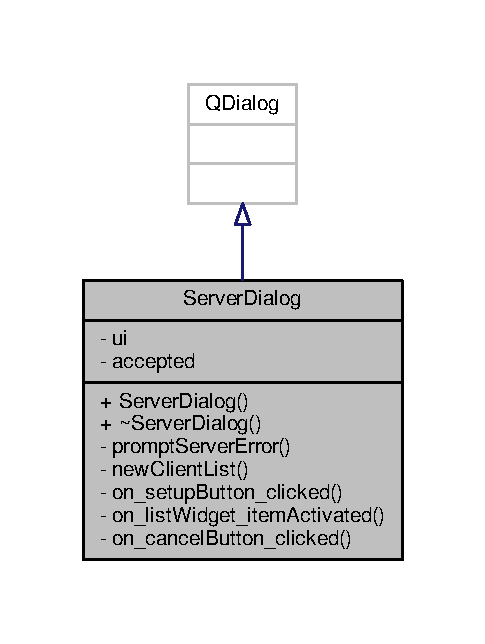
\includegraphics[width=233pt]{classServerDialog__inherit__graph}
\end{center}
\end{figure}


Collaboration diagram for Server\+Dialog\+:
\nopagebreak
\begin{figure}[H]
\begin{center}
\leavevmode
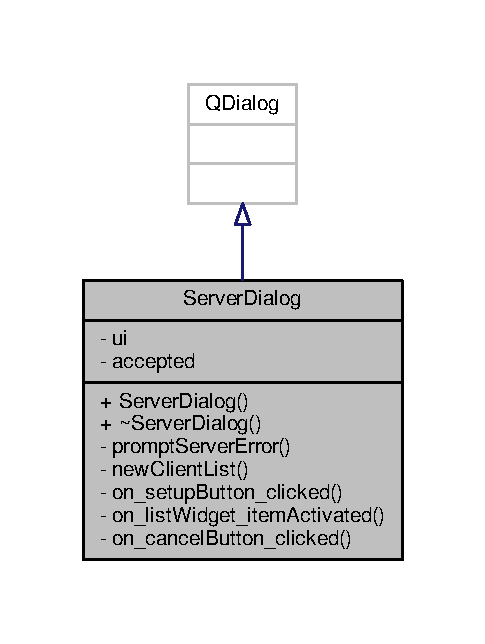
\includegraphics[width=233pt]{classServerDialog__coll__graph}
\end{center}
\end{figure}
\subsection*{Public Member Functions}
\begin{DoxyCompactItemize}
\item 
\hyperlink{classServerDialog_af2ce13bfa5d8c5d51695aaafeed1015e}{Server\+Dialog} (Q\+Widget $\ast$parent=0)
\item 
\hyperlink{classServerDialog_a05ac011efd88d4ae6f0965f7b6d3606d}{$\sim$\+Server\+Dialog} ()
\end{DoxyCompactItemize}
\subsection*{Private Slots}
\begin{DoxyCompactItemize}
\item 
void \hyperlink{classServerDialog_ad3dd1d4c4c0bbd790c21c41702bdb3c9}{prompt\+Server\+Error} ()
\item 
void \hyperlink{classServerDialog_afe38cb4103f879fc1aafffaac4be06f9}{new\+Client\+List} (const Q\+List$<$ Q\+String $>$ \&list)
\item 
void \hyperlink{classServerDialog_a54dea0fe00243a6bf5ee03069e8247b5}{on\+\_\+setup\+Button\+\_\+clicked} (bool checked)
\item 
void \hyperlink{classServerDialog_a680d9012866d27c050f1bb9a2f2c5088}{on\+\_\+list\+Widget\+\_\+item\+Activated} (Q\+List\+Widget\+Item $\ast$item)
\item 
void \hyperlink{classServerDialog_aae95a7d694dddaf6a8a66700e76e7fa5}{on\+\_\+cancel\+Button\+\_\+clicked} (bool checked)
\end{DoxyCompactItemize}
\subsection*{Private Attributes}
\begin{DoxyCompactItemize}
\item 
Ui\+::\+Server\+Dialog $\ast$ \hyperlink{classServerDialog_afa306742f46527a5a8aa54cf0e7ad3f5}{ui}
\item 
bool \hyperlink{classServerDialog_ac8aacc54e1f14195f5432c6d8983bd5c}{accepted}
\end{DoxyCompactItemize}


\subsection{Detailed Description}
Dialog to setup a server. 

\subsection{Constructor \& Destructor Documentation}
\index{Server\+Dialog@{Server\+Dialog}!Server\+Dialog@{Server\+Dialog}}
\index{Server\+Dialog@{Server\+Dialog}!Server\+Dialog@{Server\+Dialog}}
\subsubsection[{\texorpdfstring{Server\+Dialog(\+Q\+Widget $\ast$parent=0)}{ServerDialog(QWidget *parent=0)}}]{\setlength{\rightskip}{0pt plus 5cm}Server\+Dialog\+::\+Server\+Dialog (
\begin{DoxyParamCaption}
\item[{Q\+Widget $\ast$}]{parent = {\ttfamily 0}}
\end{DoxyParamCaption}
)\hspace{0.3cm}{\ttfamily [explicit]}}\hypertarget{classServerDialog_af2ce13bfa5d8c5d51695aaafeed1015e}{}\label{classServerDialog_af2ce13bfa5d8c5d51695aaafeed1015e}
\index{Server\+Dialog@{Server\+Dialog}!````~Server\+Dialog@{$\sim$\+Server\+Dialog}}
\index{````~Server\+Dialog@{$\sim$\+Server\+Dialog}!Server\+Dialog@{Server\+Dialog}}
\subsubsection[{\texorpdfstring{$\sim$\+Server\+Dialog()}{~ServerDialog()}}]{\setlength{\rightskip}{0pt plus 5cm}Server\+Dialog\+::$\sim$\+Server\+Dialog (
\begin{DoxyParamCaption}
{}
\end{DoxyParamCaption}
)}\hypertarget{classServerDialog_a05ac011efd88d4ae6f0965f7b6d3606d}{}\label{classServerDialog_a05ac011efd88d4ae6f0965f7b6d3606d}


\subsection{Member Function Documentation}
\index{Server\+Dialog@{Server\+Dialog}!new\+Client\+List@{new\+Client\+List}}
\index{new\+Client\+List@{new\+Client\+List}!Server\+Dialog@{Server\+Dialog}}
\subsubsection[{\texorpdfstring{new\+Client\+List}{newClientList}}]{\setlength{\rightskip}{0pt plus 5cm}void Server\+Dialog\+::new\+Client\+List (
\begin{DoxyParamCaption}
\item[{const Q\+List$<$ Q\+String $>$ \&}]{list}
\end{DoxyParamCaption}
)\hspace{0.3cm}{\ttfamily [private]}, {\ttfamily [slot]}}\hypertarget{classServerDialog_afe38cb4103f879fc1aafffaac4be06f9}{}\label{classServerDialog_afe38cb4103f879fc1aafffaac4be06f9}
\index{Server\+Dialog@{Server\+Dialog}!on\+\_\+cancel\+Button\+\_\+clicked@{on\+\_\+cancel\+Button\+\_\+clicked}}
\index{on\+\_\+cancel\+Button\+\_\+clicked@{on\+\_\+cancel\+Button\+\_\+clicked}!Server\+Dialog@{Server\+Dialog}}
\subsubsection[{\texorpdfstring{on\+\_\+cancel\+Button\+\_\+clicked}{on_cancelButton_clicked}}]{\setlength{\rightskip}{0pt plus 5cm}void Server\+Dialog\+::on\+\_\+cancel\+Button\+\_\+clicked (
\begin{DoxyParamCaption}
\item[{bool}]{checked}
\end{DoxyParamCaption}
)\hspace{0.3cm}{\ttfamily [private]}, {\ttfamily [slot]}}\hypertarget{classServerDialog_aae95a7d694dddaf6a8a66700e76e7fa5}{}\label{classServerDialog_aae95a7d694dddaf6a8a66700e76e7fa5}
\index{Server\+Dialog@{Server\+Dialog}!on\+\_\+list\+Widget\+\_\+item\+Activated@{on\+\_\+list\+Widget\+\_\+item\+Activated}}
\index{on\+\_\+list\+Widget\+\_\+item\+Activated@{on\+\_\+list\+Widget\+\_\+item\+Activated}!Server\+Dialog@{Server\+Dialog}}
\subsubsection[{\texorpdfstring{on\+\_\+list\+Widget\+\_\+item\+Activated}{on_listWidget_itemActivated}}]{\setlength{\rightskip}{0pt plus 5cm}void Server\+Dialog\+::on\+\_\+list\+Widget\+\_\+item\+Activated (
\begin{DoxyParamCaption}
\item[{Q\+List\+Widget\+Item $\ast$}]{item}
\end{DoxyParamCaption}
)\hspace{0.3cm}{\ttfamily [private]}, {\ttfamily [slot]}}\hypertarget{classServerDialog_a680d9012866d27c050f1bb9a2f2c5088}{}\label{classServerDialog_a680d9012866d27c050f1bb9a2f2c5088}
\index{Server\+Dialog@{Server\+Dialog}!on\+\_\+setup\+Button\+\_\+clicked@{on\+\_\+setup\+Button\+\_\+clicked}}
\index{on\+\_\+setup\+Button\+\_\+clicked@{on\+\_\+setup\+Button\+\_\+clicked}!Server\+Dialog@{Server\+Dialog}}
\subsubsection[{\texorpdfstring{on\+\_\+setup\+Button\+\_\+clicked}{on_setupButton_clicked}}]{\setlength{\rightskip}{0pt plus 5cm}void Server\+Dialog\+::on\+\_\+setup\+Button\+\_\+clicked (
\begin{DoxyParamCaption}
\item[{bool}]{checked}
\end{DoxyParamCaption}
)\hspace{0.3cm}{\ttfamily [private]}, {\ttfamily [slot]}}\hypertarget{classServerDialog_a54dea0fe00243a6bf5ee03069e8247b5}{}\label{classServerDialog_a54dea0fe00243a6bf5ee03069e8247b5}
\index{Server\+Dialog@{Server\+Dialog}!prompt\+Server\+Error@{prompt\+Server\+Error}}
\index{prompt\+Server\+Error@{prompt\+Server\+Error}!Server\+Dialog@{Server\+Dialog}}
\subsubsection[{\texorpdfstring{prompt\+Server\+Error}{promptServerError}}]{\setlength{\rightskip}{0pt plus 5cm}void Server\+Dialog\+::prompt\+Server\+Error (
\begin{DoxyParamCaption}
{}
\end{DoxyParamCaption}
)\hspace{0.3cm}{\ttfamily [private]}, {\ttfamily [slot]}}\hypertarget{classServerDialog_ad3dd1d4c4c0bbd790c21c41702bdb3c9}{}\label{classServerDialog_ad3dd1d4c4c0bbd790c21c41702bdb3c9}


\subsection{Member Data Documentation}
\index{Server\+Dialog@{Server\+Dialog}!accepted@{accepted}}
\index{accepted@{accepted}!Server\+Dialog@{Server\+Dialog}}
\subsubsection[{\texorpdfstring{accepted}{accepted}}]{\setlength{\rightskip}{0pt plus 5cm}bool Server\+Dialog\+::accepted\hspace{0.3cm}{\ttfamily [private]}}\hypertarget{classServerDialog_ac8aacc54e1f14195f5432c6d8983bd5c}{}\label{classServerDialog_ac8aacc54e1f14195f5432c6d8983bd5c}
\index{Server\+Dialog@{Server\+Dialog}!ui@{ui}}
\index{ui@{ui}!Server\+Dialog@{Server\+Dialog}}
\subsubsection[{\texorpdfstring{ui}{ui}}]{\setlength{\rightskip}{0pt plus 5cm}Ui\+::\+Server\+Dialog$\ast$ Server\+Dialog\+::ui\hspace{0.3cm}{\ttfamily [private]}}\hypertarget{classServerDialog_afa306742f46527a5a8aa54cf0e7ad3f5}{}\label{classServerDialog_afa306742f46527a5a8aa54cf0e7ad3f5}


The documentation for this class was generated from the following files\+:\begin{DoxyCompactItemize}
\item 
\hyperlink{serverdialog_8h}{serverdialog.\+h}\item 
\hyperlink{serverdialog_8cpp}{serverdialog.\+cpp}\end{DoxyCompactItemize}

\chapter{File Documentation}
\hypertarget{board_8cpp}{}\section{board.\+cpp File Reference}
\label{board_8cpp}\index{board.\+cpp@{board.\+cpp}}
{\ttfamily \#include $<$cstring$>$}\\*
{\ttfamily \#include \char`\"{}board.\+h\char`\"{}}\\*
Include dependency graph for board.\+cpp\+:
\nopagebreak
\begin{figure}[H]
\begin{center}
\leavevmode
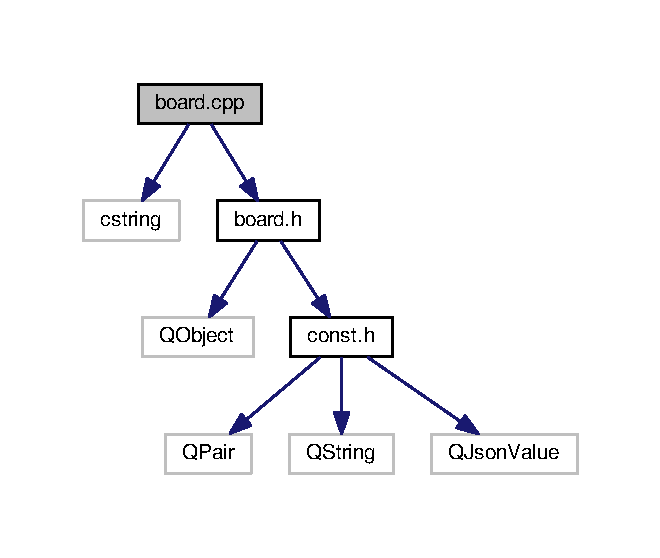
\includegraphics[width=317pt]{board_8cpp__incl}
\end{center}
\end{figure}

\hypertarget{board_8h}{}\section{board.\+h File Reference}
\label{board_8h}\index{board.\+h@{board.\+h}}
{\ttfamily \#include $<$Q\+Object$>$}\\*
{\ttfamily \#include \char`\"{}const.\+h\char`\"{}}\\*
Include dependency graph for board.\+h\+:
\nopagebreak
\begin{figure}[H]
\begin{center}
\leavevmode
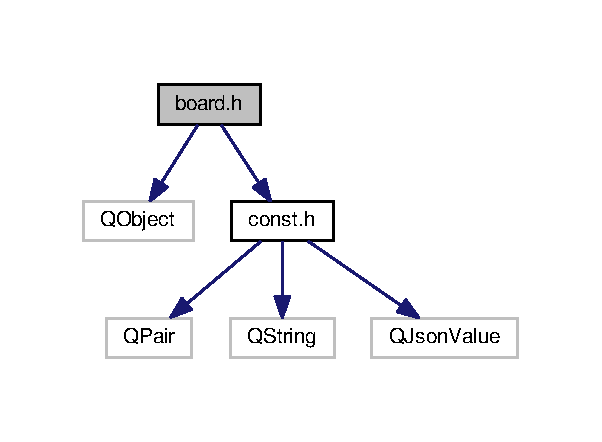
\includegraphics[width=289pt]{board_8h__incl}
\end{center}
\end{figure}
This graph shows which files directly or indirectly include this file\+:
\nopagebreak
\begin{figure}[H]
\begin{center}
\leavevmode
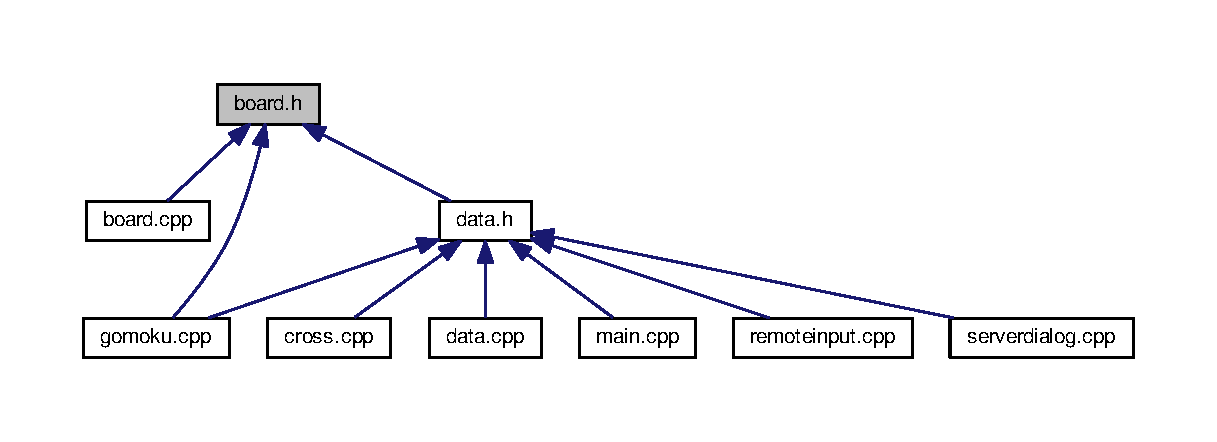
\includegraphics[width=350pt]{board_8h__dep__incl}
\end{center}
\end{figure}
\subsection*{Classes}
\begin{DoxyCompactItemize}
\item 
class \hyperlink{classBoard}{Board}
\begin{DoxyCompactList}\small\item\em \hyperlink{classGomoku}{Gomoku} board. \end{DoxyCompactList}\end{DoxyCompactItemize}

\hypertarget{const_8h}{}\section{const.\+h File Reference}
\label{const_8h}\index{const.\+h@{const.\+h}}
{\ttfamily \#include $<$Q\+Pair$>$}\\*
{\ttfamily \#include $<$Q\+String$>$}\\*
{\ttfamily \#include $<$Q\+Json\+Value$>$}\\*
Include dependency graph for const.\+h\+:
\nopagebreak
\begin{figure}[H]
\begin{center}
\leavevmode
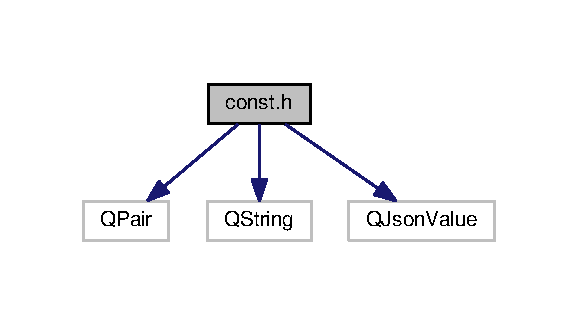
\includegraphics[width=278pt]{const_8h__incl}
\end{center}
\end{figure}
This graph shows which files directly or indirectly include this file\+:
\nopagebreak
\begin{figure}[H]
\begin{center}
\leavevmode
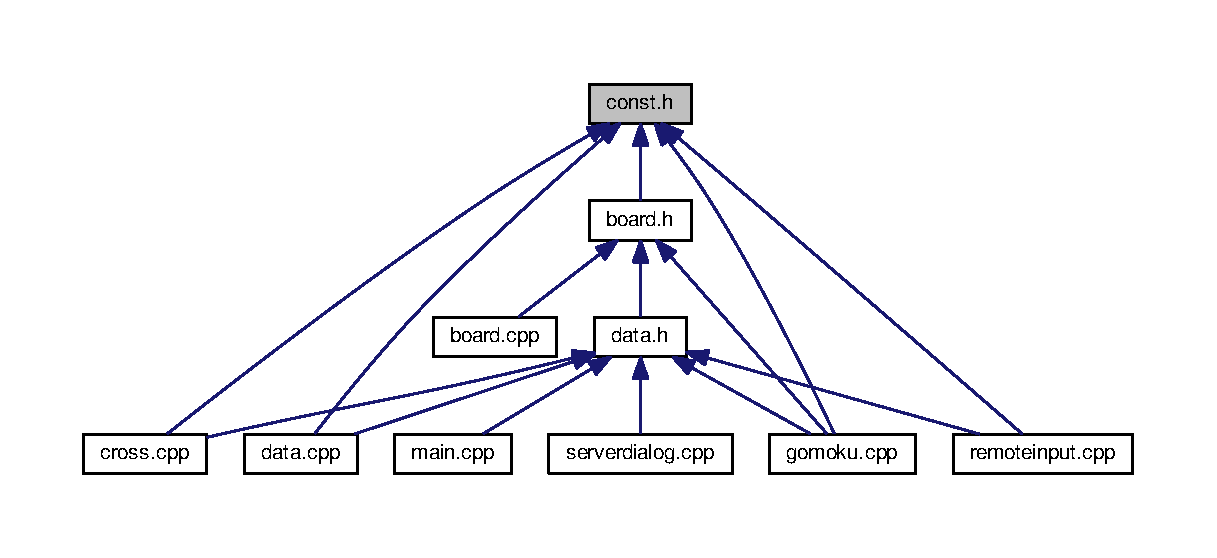
\includegraphics[width=350pt]{const_8h__dep__incl}
\end{center}
\end{figure}
\subsection*{Typedefs}
\begin{DoxyCompactItemize}
\item 
typedef Q\+Pair$<$ Q\+String, Q\+Json\+Value $>$ \hyperlink{const_8h_a54f8bd6989bd865661967393bc183790}{Json\+Key\+Value}
\end{DoxyCompactItemize}
\subsection*{Variables}
\begin{DoxyCompactItemize}
\item 
const int \hyperlink{const_8h_a11717c934f77ad5167dac5d28562d85a}{P\+O\+RT} = 8388
\begin{DoxyCompactList}\small\item\em T\+CP port. \end{DoxyCompactList}\item 
const int \hyperlink{const_8h_aa7a2b8ea2c784a4ad8b58a3262bb4f07}{B\+O\+A\+R\+D\+\_\+\+S\+I\+ZE} = 15
\end{DoxyCompactItemize}


\subsection{Typedef Documentation}
\index{const.\+h@{const.\+h}!Json\+Key\+Value@{Json\+Key\+Value}}
\index{Json\+Key\+Value@{Json\+Key\+Value}!const.\+h@{const.\+h}}
\subsubsection[{\texorpdfstring{Json\+Key\+Value}{JsonKeyValue}}]{\setlength{\rightskip}{0pt plus 5cm}typedef Q\+Pair$<$Q\+String, Q\+Json\+Value$>$ {\bf Json\+Key\+Value}}\hypertarget{const_8h_a54f8bd6989bd865661967393bc183790}{}\label{const_8h_a54f8bd6989bd865661967393bc183790}


\subsection{Variable Documentation}
\index{const.\+h@{const.\+h}!B\+O\+A\+R\+D\+\_\+\+S\+I\+ZE@{B\+O\+A\+R\+D\+\_\+\+S\+I\+ZE}}
\index{B\+O\+A\+R\+D\+\_\+\+S\+I\+ZE@{B\+O\+A\+R\+D\+\_\+\+S\+I\+ZE}!const.\+h@{const.\+h}}
\subsubsection[{\texorpdfstring{B\+O\+A\+R\+D\+\_\+\+S\+I\+ZE}{BOARD_SIZE}}]{\setlength{\rightskip}{0pt plus 5cm}const int B\+O\+A\+R\+D\+\_\+\+S\+I\+ZE = 15}\hypertarget{const_8h_aa7a2b8ea2c784a4ad8b58a3262bb4f07}{}\label{const_8h_aa7a2b8ea2c784a4ad8b58a3262bb4f07}
\index{const.\+h@{const.\+h}!P\+O\+RT@{P\+O\+RT}}
\index{P\+O\+RT@{P\+O\+RT}!const.\+h@{const.\+h}}
\subsubsection[{\texorpdfstring{P\+O\+RT}{PORT}}]{\setlength{\rightskip}{0pt plus 5cm}const int P\+O\+RT = 8388}\hypertarget{const_8h_a11717c934f77ad5167dac5d28562d85a}{}\label{const_8h_a11717c934f77ad5167dac5d28562d85a}


T\+CP port. 


\hypertarget{cross_8cpp}{}\section{cross.\+cpp File Reference}
\label{cross_8cpp}\index{cross.\+cpp@{cross.\+cpp}}
{\ttfamily \#include $<$algorithm$>$}\\*
{\ttfamily \#include $<$Q\+Pen$>$}\\*
{\ttfamily \#include $<$Q\+Brush$>$}\\*
{\ttfamily \#include $<$Q\+Color$>$}\\*
{\ttfamily \#include $<$Q\+Pixmap$>$}\\*
{\ttfamily \#include $<$Q\+Painter$>$}\\*
{\ttfamily \#include \char`\"{}data.\+h\char`\"{}}\\*
{\ttfamily \#include \char`\"{}cross.\+h\char`\"{}}\\*
{\ttfamily \#include \char`\"{}const.\+h\char`\"{}}\\*
Include dependency graph for cross.\+cpp\+:
\nopagebreak
\begin{figure}[H]
\begin{center}
\leavevmode
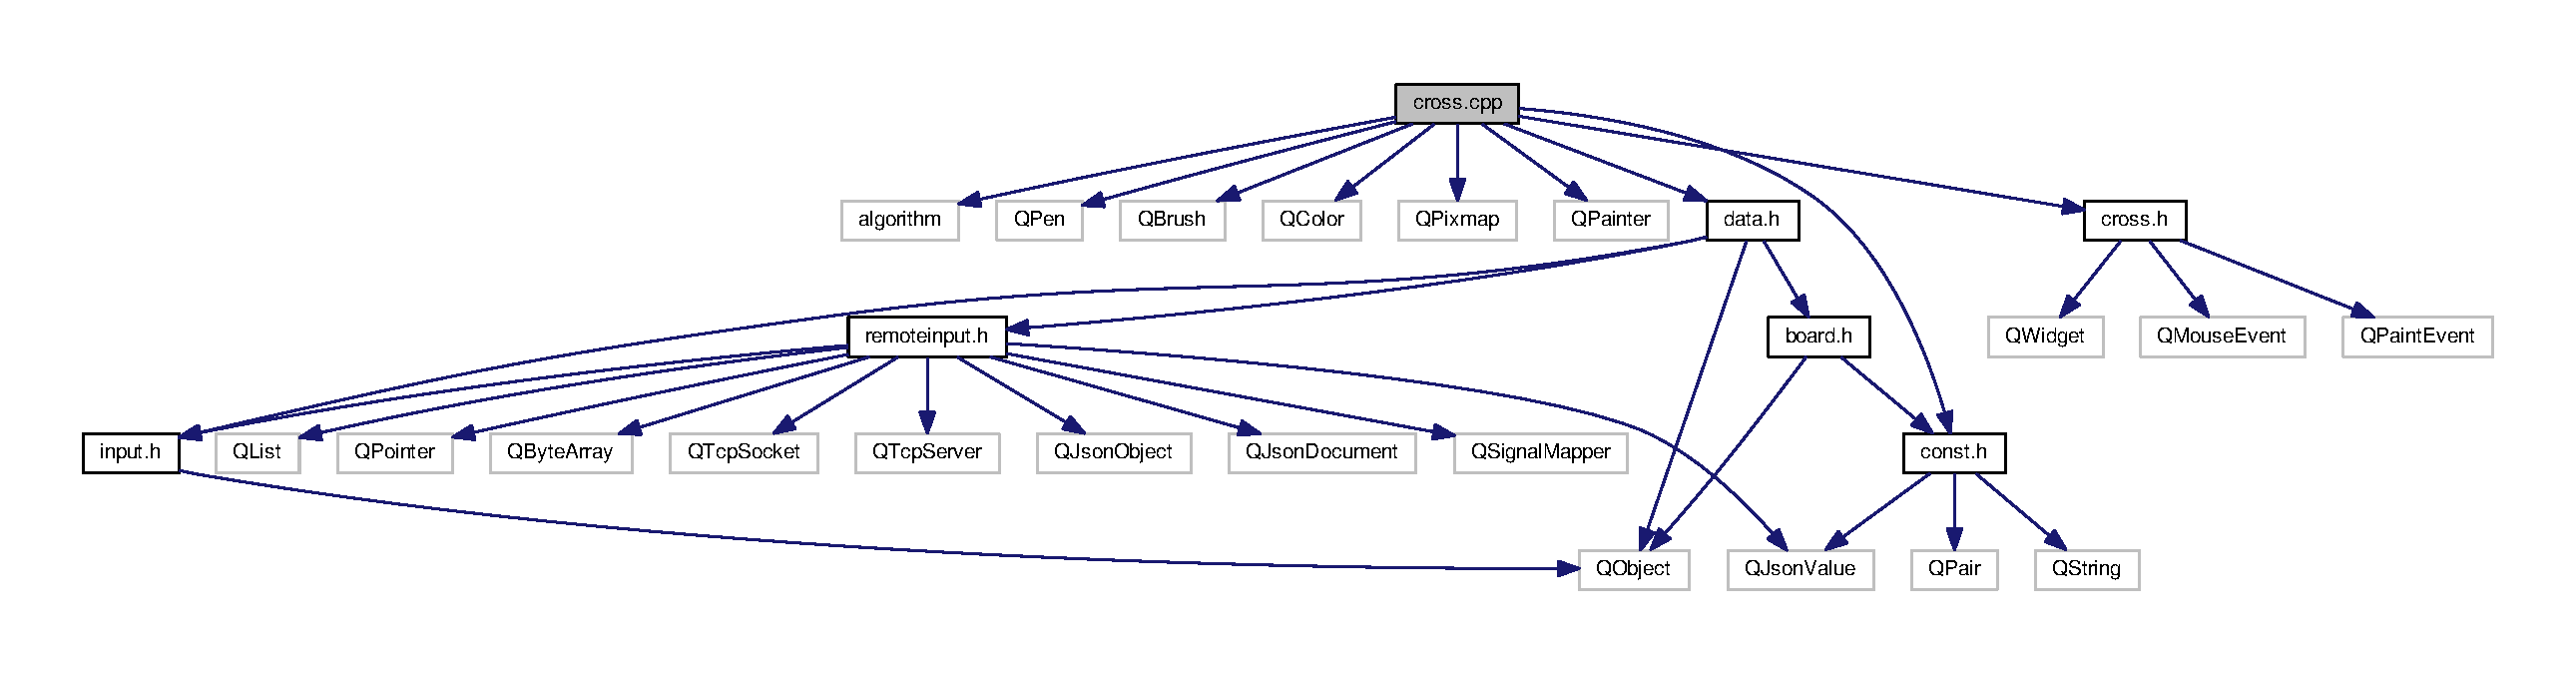
\includegraphics[width=350pt]{cross_8cpp__incl}
\end{center}
\end{figure}

\hypertarget{cross_8h}{}\section{cross.\+h File Reference}
\label{cross_8h}\index{cross.\+h@{cross.\+h}}
{\ttfamily \#include $<$Q\+Widget$>$}\\*
{\ttfamily \#include $<$Q\+Mouse\+Event$>$}\\*
{\ttfamily \#include $<$Q\+Paint\+Event$>$}\\*
Include dependency graph for cross.\+h\+:
\nopagebreak
\begin{figure}[H]
\begin{center}
\leavevmode
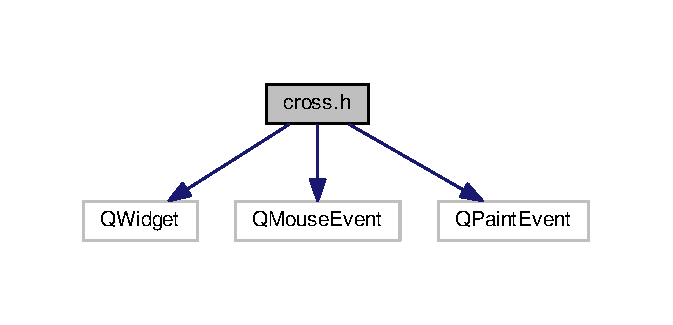
\includegraphics[width=323pt]{cross_8h__incl}
\end{center}
\end{figure}
This graph shows which files directly or indirectly include this file\+:
\nopagebreak
\begin{figure}[H]
\begin{center}
\leavevmode
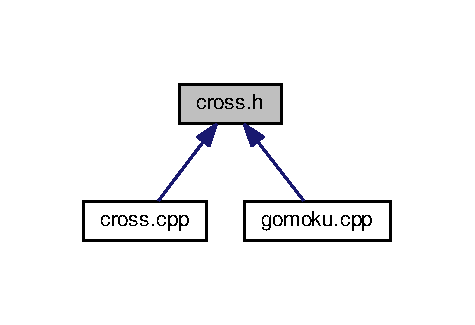
\includegraphics[width=228pt]{cross_8h__dep__incl}
\end{center}
\end{figure}
\subsection*{Classes}
\begin{DoxyCompactItemize}
\item 
class \hyperlink{classCross}{Cross}
\begin{DoxyCompactList}\small\item\em A \hyperlink{classCross}{Cross} on the board. \end{DoxyCompactList}\end{DoxyCompactItemize}

\hypertarget{data_8cpp}{}\section{data.\+cpp File Reference}
\label{data_8cpp}\index{data.\+cpp@{data.\+cpp}}
{\ttfamily \#include $<$cstdlib$>$}\\*
{\ttfamily \#include $<$Q\+Debug$>$}\\*
{\ttfamily \#include $<$Q\+Message\+Box$>$}\\*
{\ttfamily \#include \char`\"{}data.\+h\char`\"{}}\\*
{\ttfamily \#include \char`\"{}const.\+h\char`\"{}}\\*
{\ttfamily \#include \char`\"{}input.\+h\char`\"{}}\\*
{\ttfamily \#include \char`\"{}remoteinput.\+h\char`\"{}}\\*
Include dependency graph for data.\+cpp\+:
\nopagebreak
\begin{figure}[H]
\begin{center}
\leavevmode
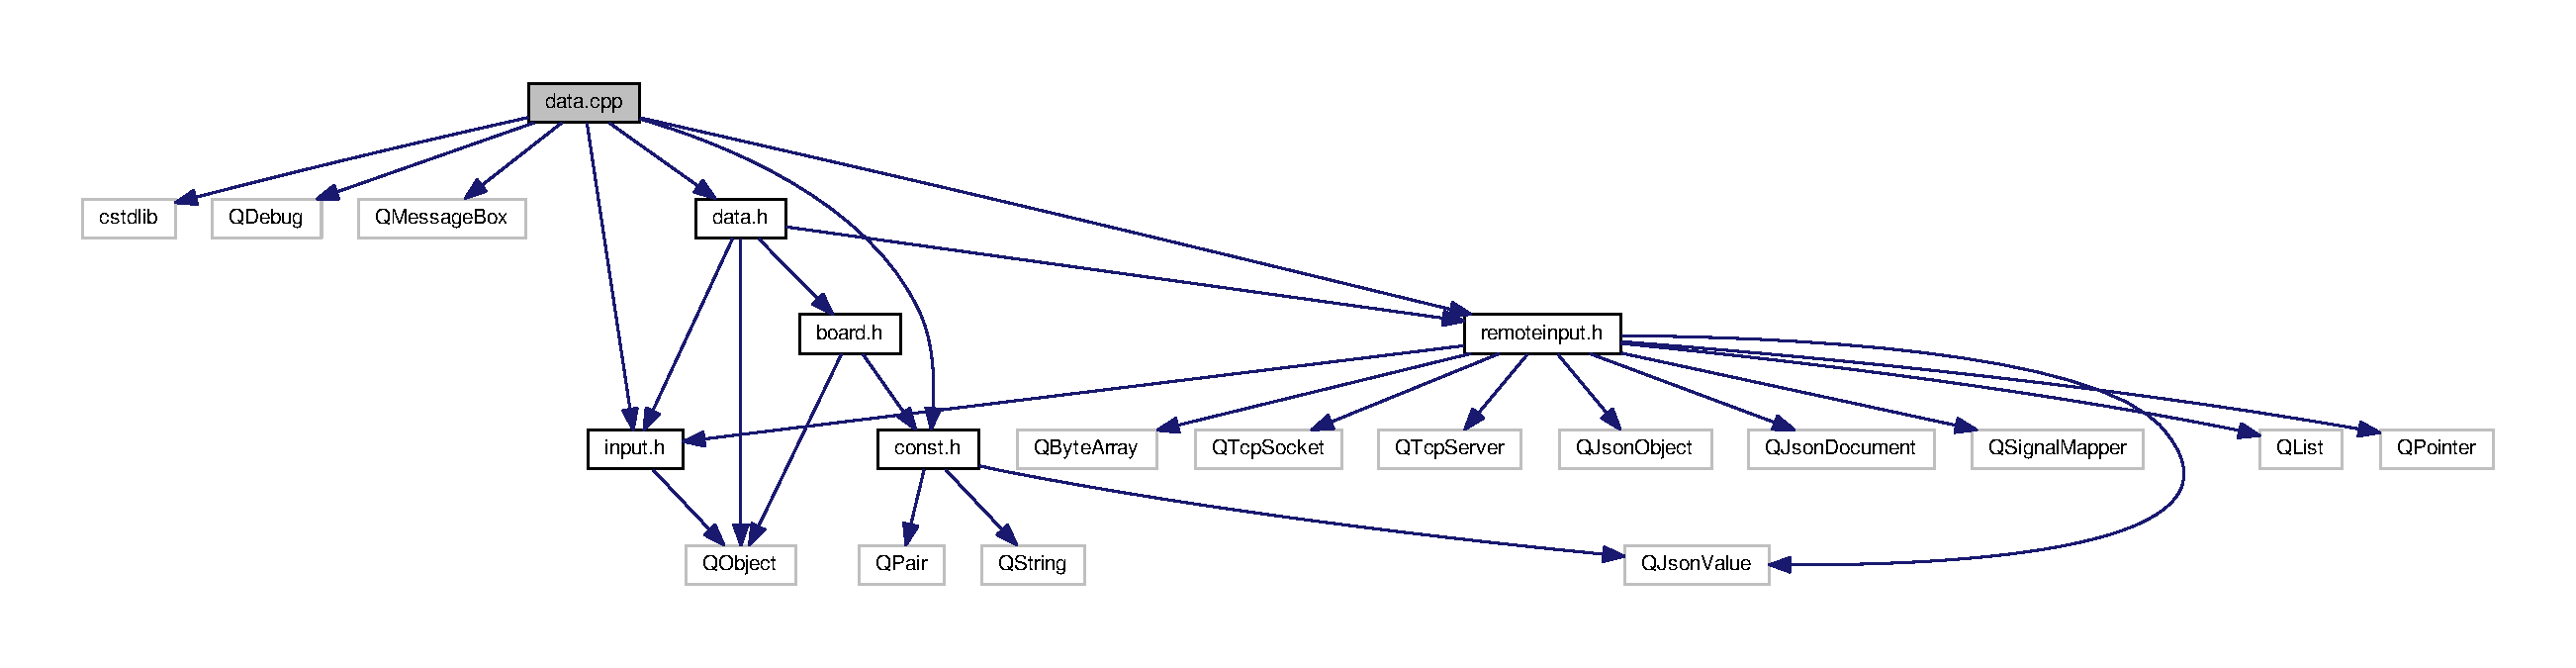
\includegraphics[width=350pt]{data_8cpp__incl}
\end{center}
\end{figure}

\hypertarget{data_8h}{}\section{data.\+h File Reference}
\label{data_8h}\index{data.\+h@{data.\+h}}
{\ttfamily \#include $<$Q\+Object$>$}\\*
{\ttfamily \#include \char`\"{}board.\+h\char`\"{}}\\*
{\ttfamily \#include \char`\"{}input.\+h\char`\"{}}\\*
{\ttfamily \#include \char`\"{}remoteinput.\+h\char`\"{}}\\*
Include dependency graph for data.\+h\+:
\nopagebreak
\begin{figure}[H]
\begin{center}
\leavevmode
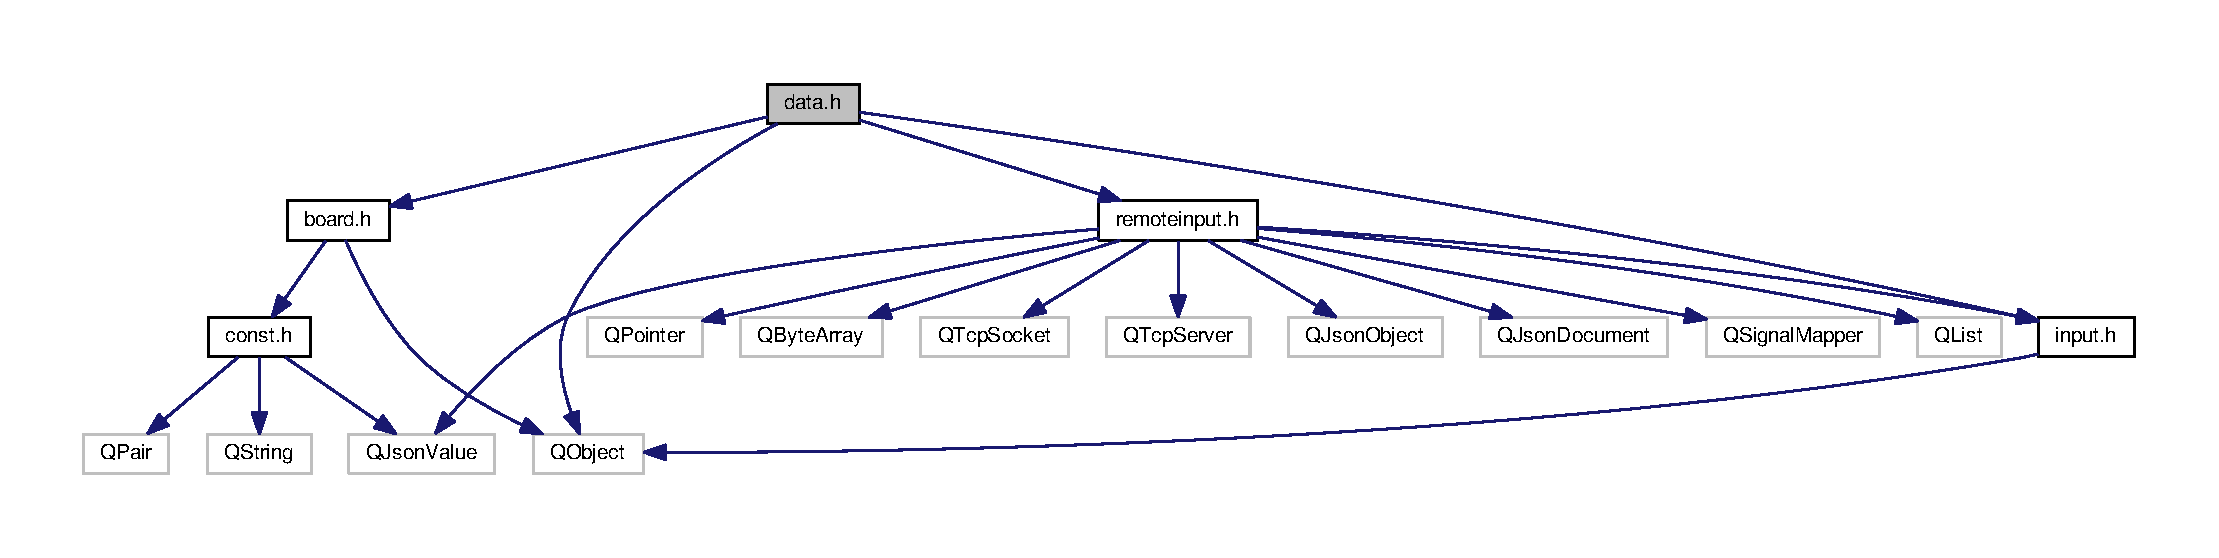
\includegraphics[width=350pt]{data_8h__incl}
\end{center}
\end{figure}
This graph shows which files directly or indirectly include this file\+:
\nopagebreak
\begin{figure}[H]
\begin{center}
\leavevmode
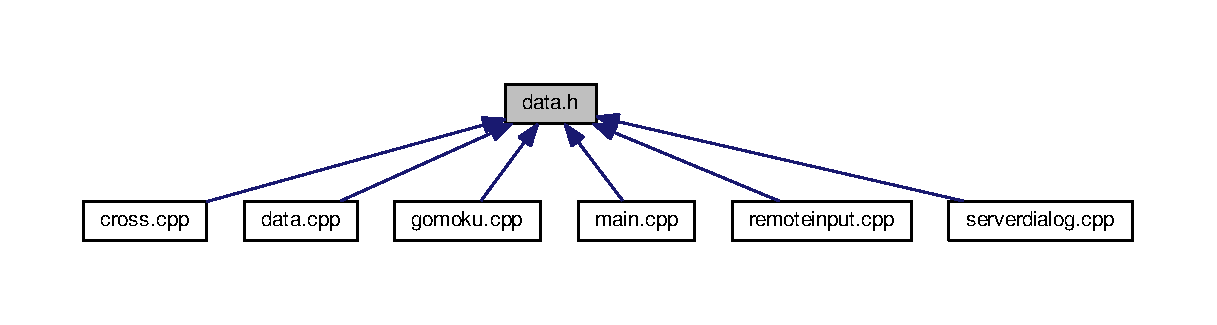
\includegraphics[width=350pt]{data_8h__dep__incl}
\end{center}
\end{figure}
\subsection*{Classes}
\begin{DoxyCompactItemize}
\item 
class \hyperlink{classData}{Data}
\begin{DoxyCompactList}\small\item\em Manages all data. \end{DoxyCompactList}\end{DoxyCompactItemize}

\hypertarget{gomoku_8cpp}{}\section{gomoku.\+cpp File Reference}
\label{gomoku_8cpp}\index{gomoku.\+cpp@{gomoku.\+cpp}}
{\ttfamily \#include $<$Q\+Debug$>$}\\*
{\ttfamily \#include $<$Q\+Line\+Edit$>$}\\*
{\ttfamily \#include $<$Q\+Message\+Box$>$}\\*
{\ttfamily \#include $<$Q\+Grid\+Layout$>$}\\*
{\ttfamily \#include $<$Q\+Input\+Dialog$>$}\\*
{\ttfamily \#include \char`\"{}data.\+h\char`\"{}}\\*
{\ttfamily \#include \char`\"{}board.\+h\char`\"{}}\\*
{\ttfamily \#include \char`\"{}cross.\+h\char`\"{}}\\*
{\ttfamily \#include \char`\"{}input.\+h\char`\"{}}\\*
{\ttfamily \#include \char`\"{}const.\+h\char`\"{}}\\*
{\ttfamily \#include \char`\"{}gomoku.\+h\char`\"{}}\\*
{\ttfamily \#include \char`\"{}ipinput.\+h\char`\"{}}\\*
{\ttfamily \#include \char`\"{}ui\+\_\+gomoku.\+h\char`\"{}}\\*
{\ttfamily \#include \char`\"{}remoteinput.\+h\char`\"{}}\\*
{\ttfamily \#include \char`\"{}serverdialog.\+h\char`\"{}}\\*
Include dependency graph for gomoku.\+cpp\+:
\nopagebreak
\begin{figure}[H]
\begin{center}
\leavevmode
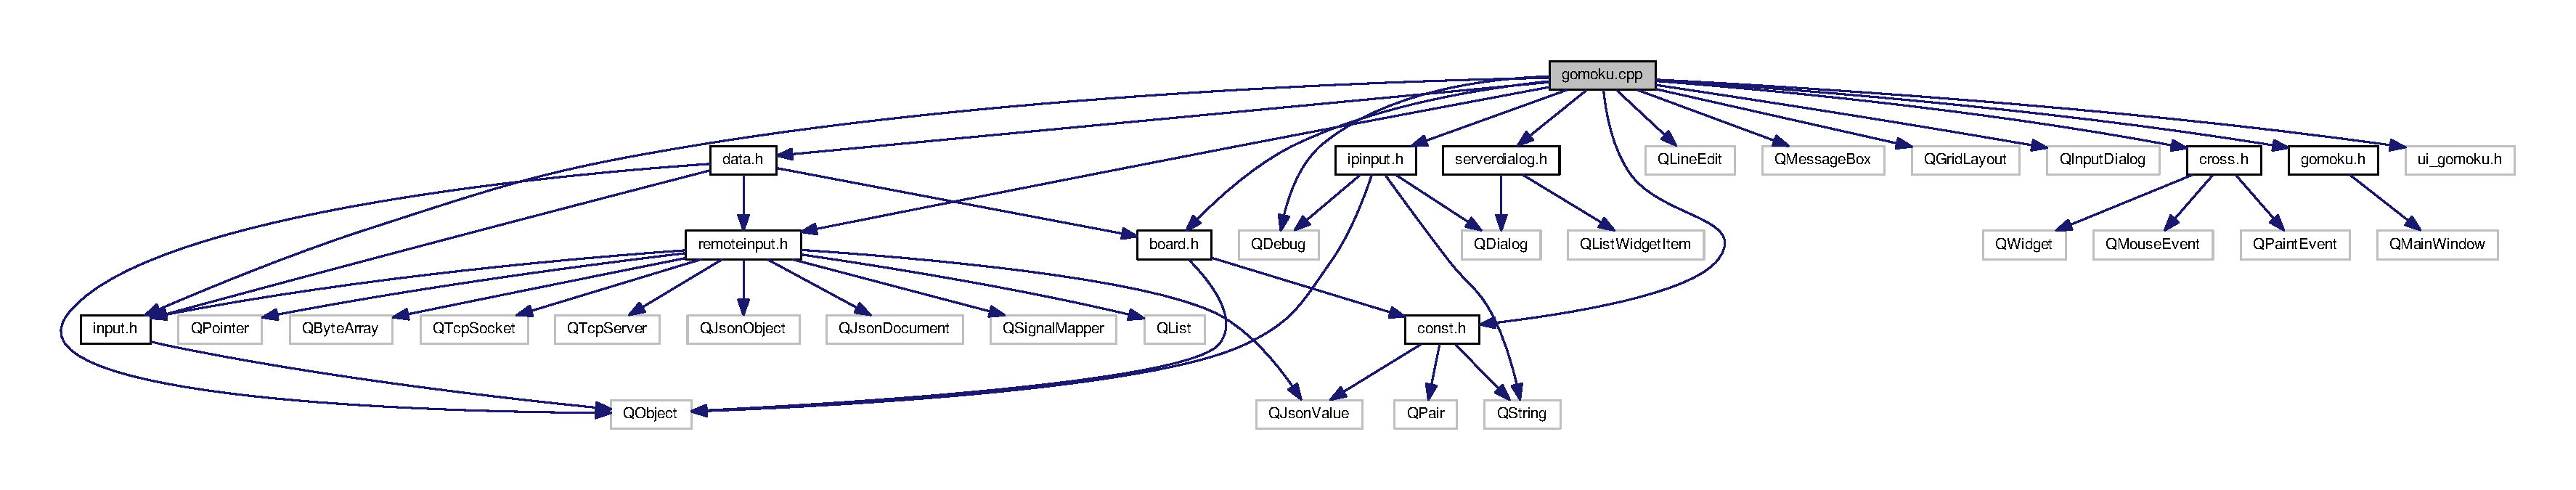
\includegraphics[width=350pt]{gomoku_8cpp__incl}
\end{center}
\end{figure}

\hypertarget{gomoku_8h}{}\section{gomoku.\+h File Reference}
\label{gomoku_8h}\index{gomoku.\+h@{gomoku.\+h}}
{\ttfamily \#include $<$Q\+Main\+Window$>$}\\*
Include dependency graph for gomoku.\+h\+:
\nopagebreak
\begin{figure}[H]
\begin{center}
\leavevmode
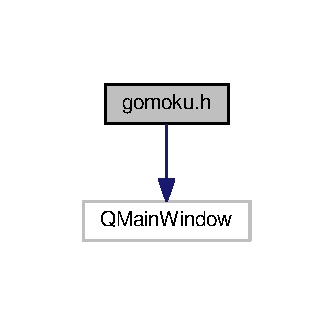
\includegraphics[width=160pt]{gomoku_8h__incl}
\end{center}
\end{figure}
This graph shows which files directly or indirectly include this file\+:
\nopagebreak
\begin{figure}[H]
\begin{center}
\leavevmode
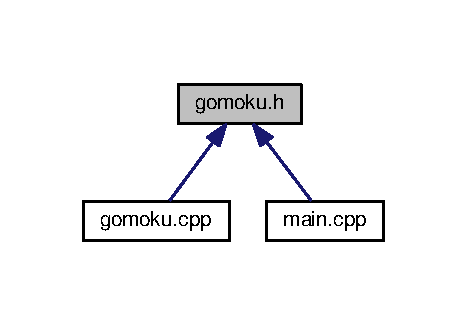
\includegraphics[width=224pt]{gomoku_8h__dep__incl}
\end{center}
\end{figure}
\subsection*{Classes}
\begin{DoxyCompactItemize}
\item 
class \hyperlink{classGomoku}{Gomoku}
\begin{DoxyCompactList}\small\item\em Main window. \end{DoxyCompactList}\end{DoxyCompactItemize}
\subsection*{Namespaces}
\begin{DoxyCompactItemize}
\item 
 \hyperlink{namespaceUi}{Ui}
\end{DoxyCompactItemize}

\hypertarget{input_8cpp}{}\section{input.\+cpp File Reference}
\label{input_8cpp}\index{input.\+cpp@{input.\+cpp}}
{\ttfamily \#include \char`\"{}input.\+h\char`\"{}}\\*
Include dependency graph for input.\+cpp\+:
\nopagebreak
\begin{figure}[H]
\begin{center}
\leavevmode
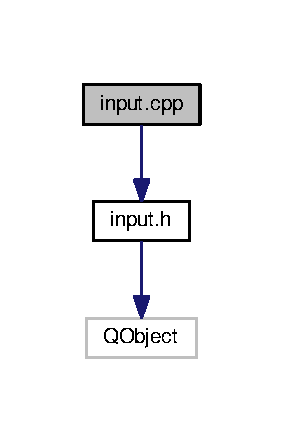
\includegraphics[width=136pt]{input_8cpp__incl}
\end{center}
\end{figure}

\hypertarget{input_8h}{}\section{input.\+h File Reference}
\label{input_8h}\index{input.\+h@{input.\+h}}
{\ttfamily \#include $<$Q\+Object$>$}\\*
Include dependency graph for input.\+h\+:
\nopagebreak
\begin{figure}[H]
\begin{center}
\leavevmode
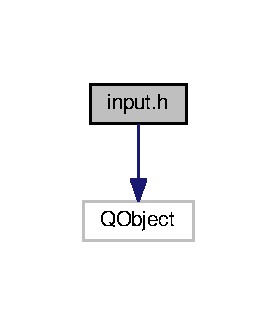
\includegraphics[width=133pt]{input_8h__incl}
\end{center}
\end{figure}
This graph shows which files directly or indirectly include this file\+:
\nopagebreak
\begin{figure}[H]
\begin{center}
\leavevmode
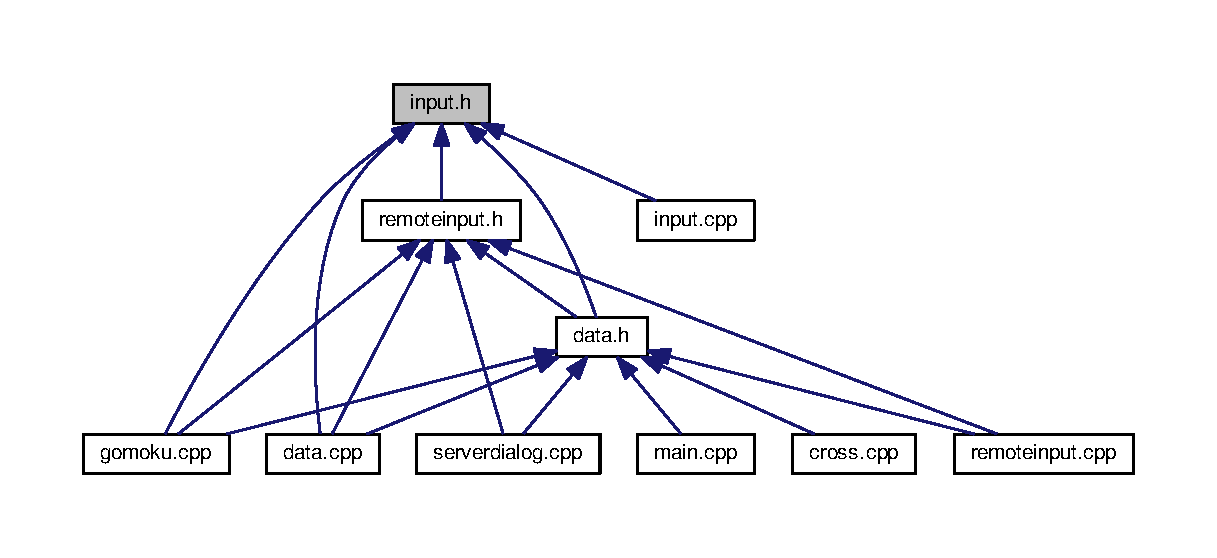
\includegraphics[width=350pt]{input_8h__dep__incl}
\end{center}
\end{figure}
\subsection*{Classes}
\begin{DoxyCompactItemize}
\item 
class \hyperlink{classInput}{Input}
\begin{DoxyCompactList}\small\item\em Base class for user input from local or remote. \end{DoxyCompactList}\end{DoxyCompactItemize}

\hypertarget{ipinput_8cpp}{}\section{ipinput.\+cpp File Reference}
\label{ipinput_8cpp}\index{ipinput.\+cpp@{ipinput.\+cpp}}
{\ttfamily \#include $<$Q\+Debug$>$}\\*
{\ttfamily \#include \char`\"{}ipinput.\+h\char`\"{}}\\*
{\ttfamily \#include \char`\"{}ui\+\_\+ipinput.\+h\char`\"{}}\\*
Include dependency graph for ipinput.\+cpp\+:
\nopagebreak
\begin{figure}[H]
\begin{center}
\leavevmode
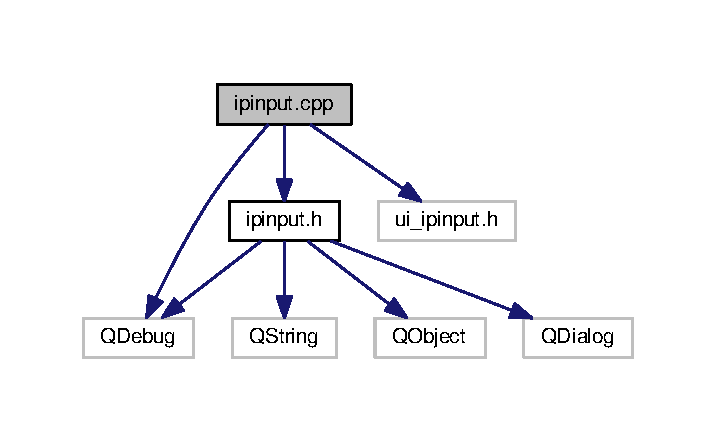
\includegraphics[width=344pt]{ipinput_8cpp__incl}
\end{center}
\end{figure}

\hypertarget{ipinput_8h}{}\section{ipinput.\+h File Reference}
\label{ipinput_8h}\index{ipinput.\+h@{ipinput.\+h}}
{\ttfamily \#include $<$Q\+Debug$>$}\\*
{\ttfamily \#include $<$Q\+String$>$}\\*
{\ttfamily \#include $<$Q\+Object$>$}\\*
{\ttfamily \#include $<$Q\+Dialog$>$}\\*
Include dependency graph for ipinput.\+h\+:
\nopagebreak
\begin{figure}[H]
\begin{center}
\leavevmode
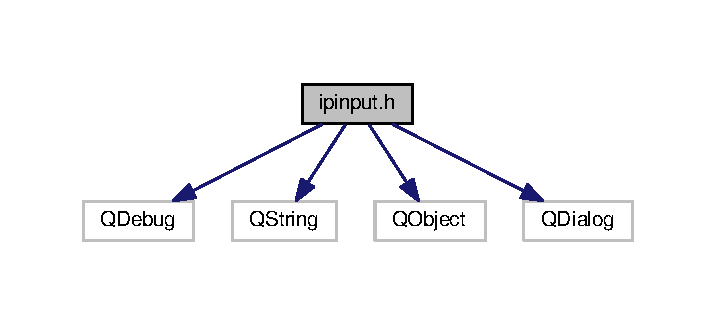
\includegraphics[width=344pt]{ipinput_8h__incl}
\end{center}
\end{figure}
This graph shows which files directly or indirectly include this file\+:
\nopagebreak
\begin{figure}[H]
\begin{center}
\leavevmode
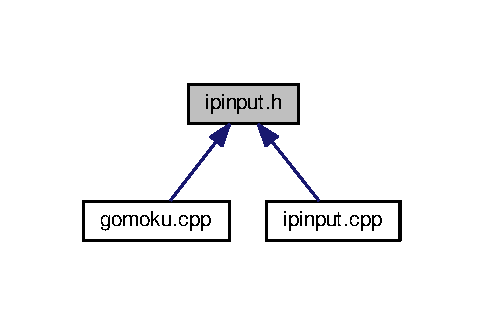
\includegraphics[width=232pt]{ipinput_8h__dep__incl}
\end{center}
\end{figure}
\subsection*{Classes}
\begin{DoxyCompactItemize}
\item 
class \hyperlink{classIpInput}{Ip\+Input}
\item 
class \hyperlink{classGetter}{Getter}
\end{DoxyCompactItemize}
\subsection*{Namespaces}
\begin{DoxyCompactItemize}
\item 
 \hyperlink{namespaceUi}{Ui}
\end{DoxyCompactItemize}

\hypertarget{main_8cpp}{}\section{main.\+cpp File Reference}
\label{main_8cpp}\index{main.\+cpp@{main.\+cpp}}
{\ttfamily \#include $<$ctime$>$}\\*
{\ttfamily \#include $<$cstdlib$>$}\\*
{\ttfamily \#include $<$Q\+Application$>$}\\*
{\ttfamily \#include \char`\"{}data.\+h\char`\"{}}\\*
{\ttfamily \#include \char`\"{}gomoku.\+h\char`\"{}}\\*
Include dependency graph for main.\+cpp\+:
\nopagebreak
\begin{figure}[H]
\begin{center}
\leavevmode
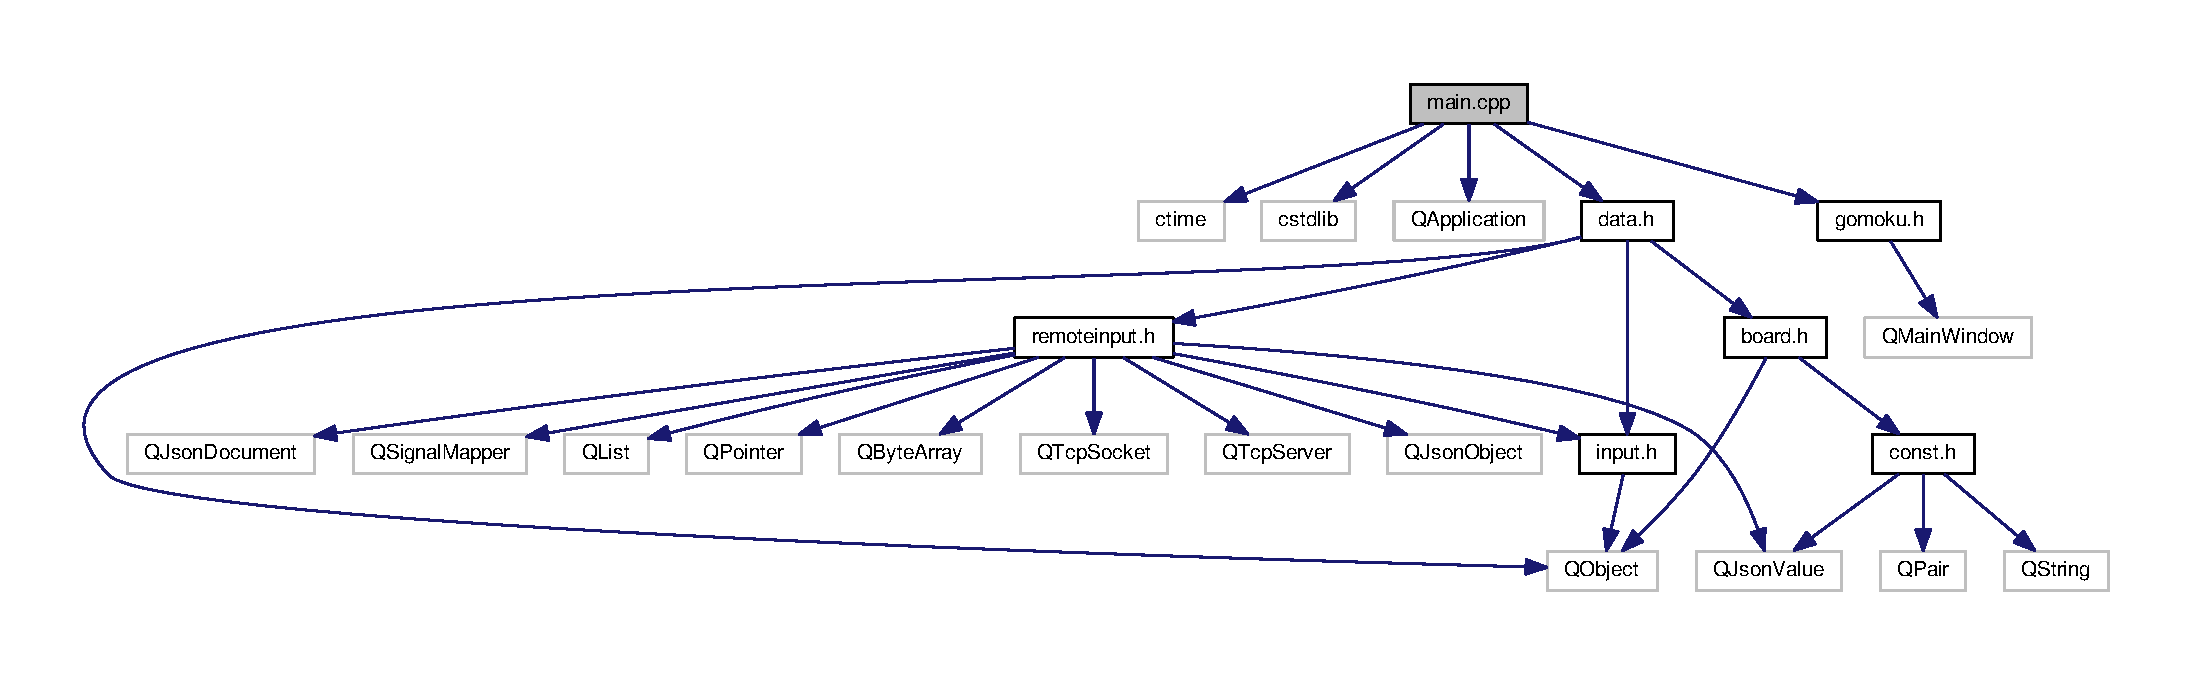
\includegraphics[width=350pt]{main_8cpp__incl}
\end{center}
\end{figure}
\subsection*{Functions}
\begin{DoxyCompactItemize}
\item 
int \hyperlink{main_8cpp_a0ddf1224851353fc92bfbff6f499fa97}{main} (int argc, char $\ast$argv\mbox{[}$\,$\mbox{]})
\end{DoxyCompactItemize}


\subsection{Function Documentation}
\index{main.\+cpp@{main.\+cpp}!main@{main}}
\index{main@{main}!main.\+cpp@{main.\+cpp}}
\subsubsection[{\texorpdfstring{main(int argc, char $\ast$argv[])}{main(int argc, char *argv[])}}]{\setlength{\rightskip}{0pt plus 5cm}int main (
\begin{DoxyParamCaption}
\item[{int}]{argc, }
\item[{char $\ast$}]{argv\mbox{[}$\,$\mbox{]}}
\end{DoxyParamCaption}
)}\hypertarget{main_8cpp_a0ddf1224851353fc92bfbff6f499fa97}{}\label{main_8cpp_a0ddf1224851353fc92bfbff6f499fa97}

\hypertarget{remoteinput_8cpp}{}\section{remoteinput.\+cpp File Reference}
\label{remoteinput_8cpp}\index{remoteinput.\+cpp@{remoteinput.\+cpp}}
{\ttfamily \#include $<$Q\+Debug$>$}\\*
{\ttfamily \#include $<$Q\+Tcp\+Socket$>$}\\*
{\ttfamily \#include $<$Q\+Byte\+Array$>$}\\*
{\ttfamily \#include $<$Q\+Host\+Address$>$}\\*
{\ttfamily \#include $<$Q\+Json\+Parse\+Error$>$}\\*
{\ttfamily \#include \char`\"{}data.\+h\char`\"{}}\\*
{\ttfamily \#include \char`\"{}const.\+h\char`\"{}}\\*
{\ttfamily \#include \char`\"{}remoteinput.\+h\char`\"{}}\\*
Include dependency graph for remoteinput.\+cpp\+:
\nopagebreak
\begin{figure}[H]
\begin{center}
\leavevmode
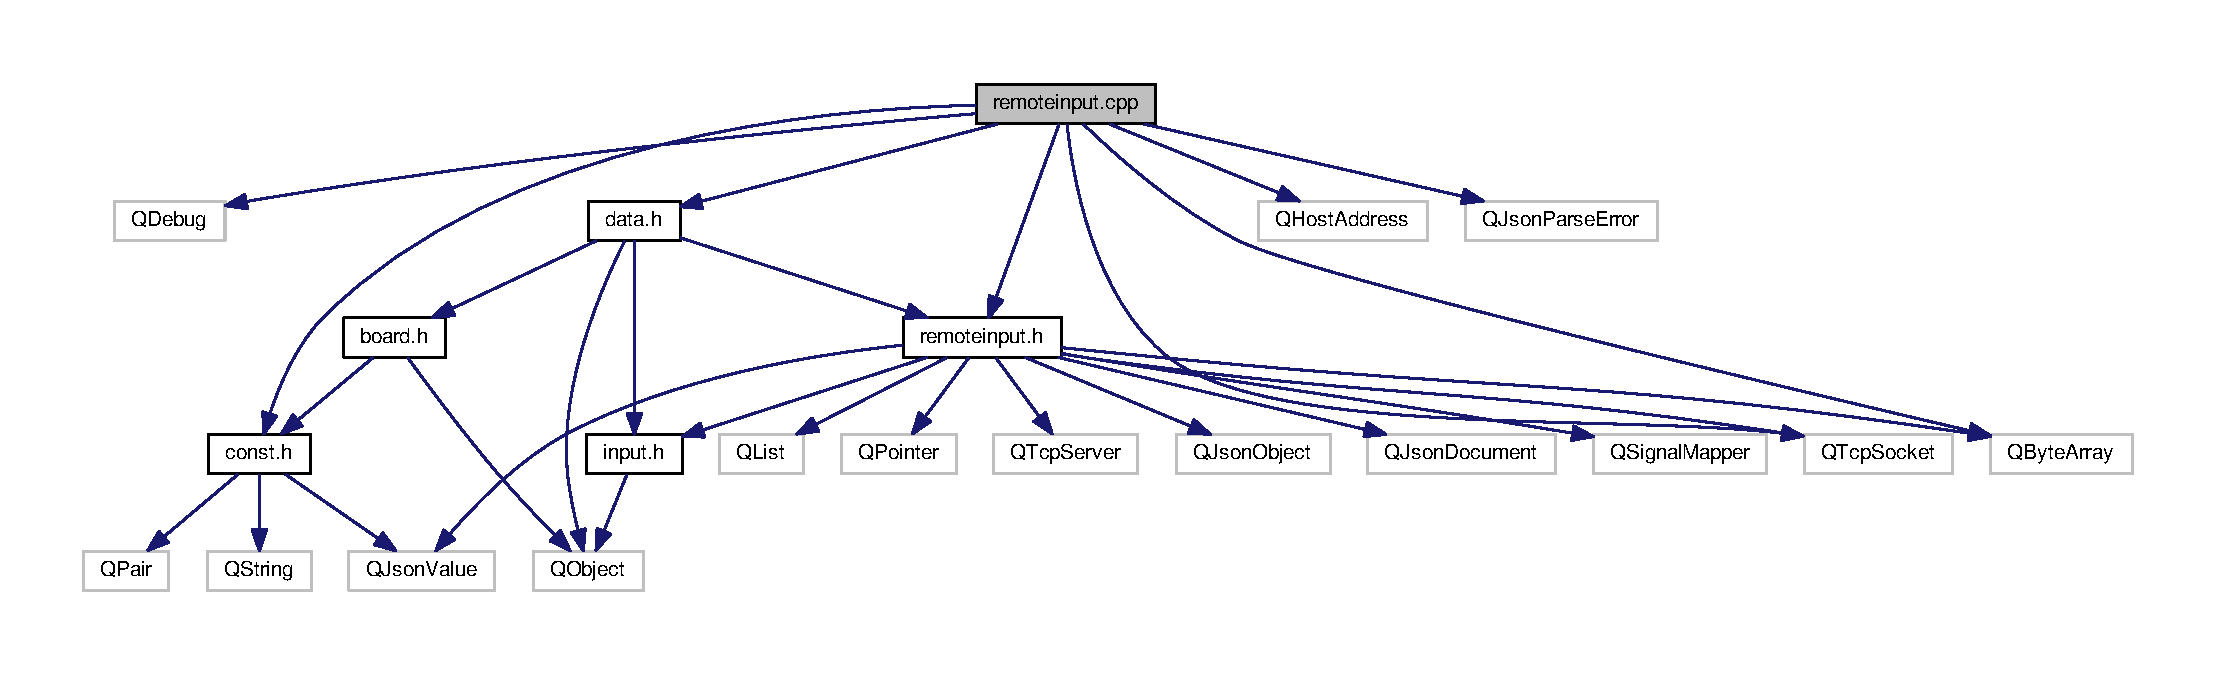
\includegraphics[width=350pt]{remoteinput_8cpp__incl}
\end{center}
\end{figure}

\hypertarget{remoteinput_8h}{}\section{remoteinput.\+h File Reference}
\label{remoteinput_8h}\index{remoteinput.\+h@{remoteinput.\+h}}
{\ttfamily \#include $<$Q\+List$>$}\\*
{\ttfamily \#include $<$Q\+Pointer$>$}\\*
{\ttfamily \#include $<$Q\+Byte\+Array$>$}\\*
{\ttfamily \#include $<$Q\+Tcp\+Socket$>$}\\*
{\ttfamily \#include $<$Q\+Tcp\+Server$>$}\\*
{\ttfamily \#include $<$Q\+Json\+Value$>$}\\*
{\ttfamily \#include $<$Q\+Json\+Object$>$}\\*
{\ttfamily \#include $<$Q\+Json\+Document$>$}\\*
{\ttfamily \#include $<$Q\+Signal\+Mapper$>$}\\*
{\ttfamily \#include \char`\"{}input.\+h\char`\"{}}\\*
Include dependency graph for remoteinput.\+h\+:
\nopagebreak
\begin{figure}[H]
\begin{center}
\leavevmode
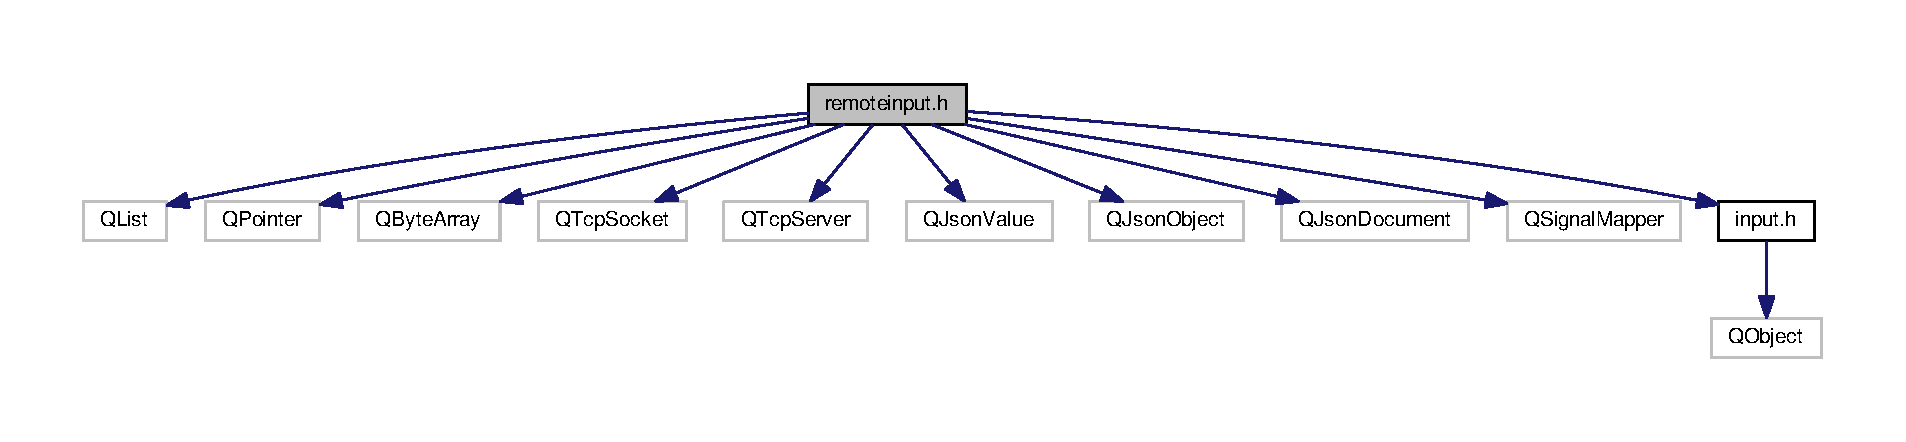
\includegraphics[width=350pt]{remoteinput_8h__incl}
\end{center}
\end{figure}
This graph shows which files directly or indirectly include this file\+:
\nopagebreak
\begin{figure}[H]
\begin{center}
\leavevmode
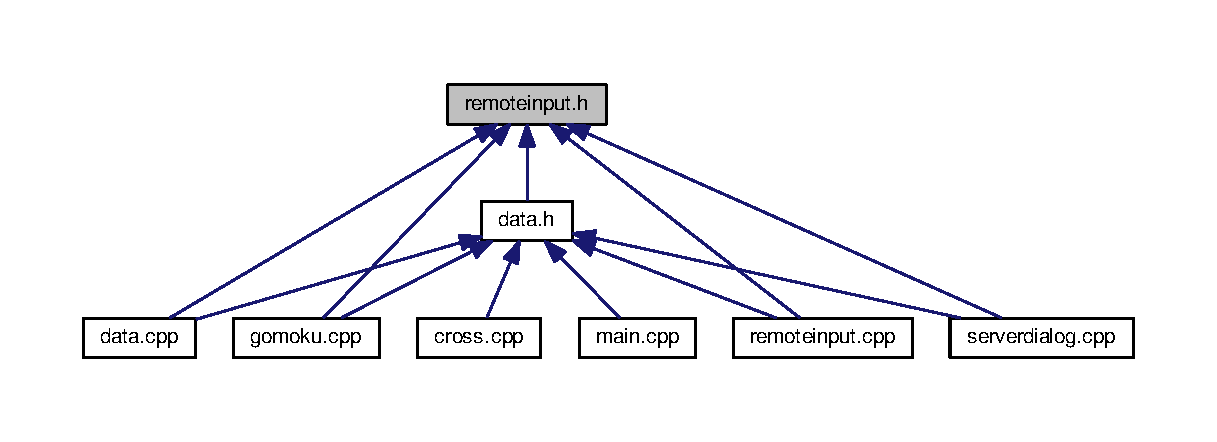
\includegraphics[width=350pt]{remoteinput_8h__dep__incl}
\end{center}
\end{figure}
\subsection*{Classes}
\begin{DoxyCompactItemize}
\item 
class \hyperlink{classRemoteInput}{Remote\+Input}
\begin{DoxyCompactList}\small\item\em User input from remote. \end{DoxyCompactList}\end{DoxyCompactItemize}

\hypertarget{serverdialog_8cpp}{}\section{serverdialog.\+cpp File Reference}
\label{serverdialog_8cpp}\index{serverdialog.\+cpp@{serverdialog.\+cpp}}
{\ttfamily \#include $<$Q\+Debug$>$}\\*
{\ttfamily \#include $<$Q\+Message\+Box$>$}\\*
{\ttfamily \#include $<$Q\+Host\+Address$>$}\\*
{\ttfamily \#include $<$Q\+Network\+Interface$>$}\\*
{\ttfamily \#include \char`\"{}data.\+h\char`\"{}}\\*
{\ttfamily \#include \char`\"{}remoteinput.\+h\char`\"{}}\\*
{\ttfamily \#include \char`\"{}serverdialog.\+h\char`\"{}}\\*
{\ttfamily \#include \char`\"{}ui\+\_\+serverdialog.\+h\char`\"{}}\\*
Include dependency graph for serverdialog.\+cpp\+:
\nopagebreak
\begin{figure}[H]
\begin{center}
\leavevmode
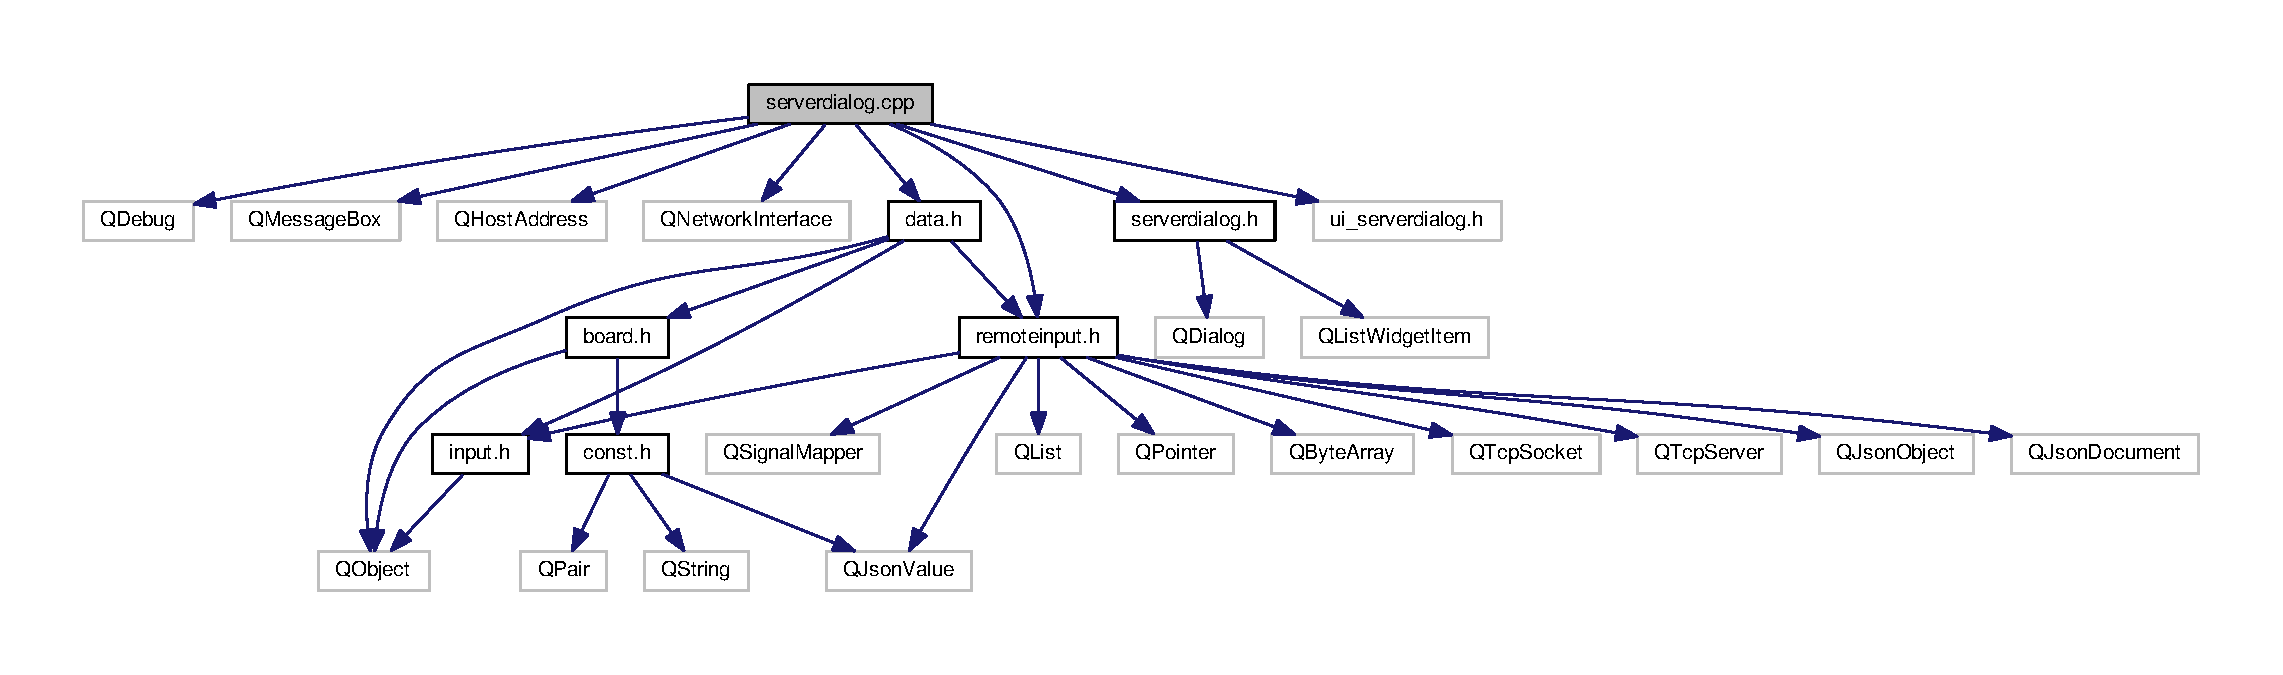
\includegraphics[width=350pt]{serverdialog_8cpp__incl}
\end{center}
\end{figure}

\hypertarget{serverdialog_8h}{}\section{serverdialog.\+h File Reference}
\label{serverdialog_8h}\index{serverdialog.\+h@{serverdialog.\+h}}
{\ttfamily \#include $<$Q\+Dialog$>$}\\*
{\ttfamily \#include $<$Q\+List\+Widget\+Item$>$}\\*
Include dependency graph for serverdialog.\+h\+:
\nopagebreak
\begin{figure}[H]
\begin{center}
\leavevmode
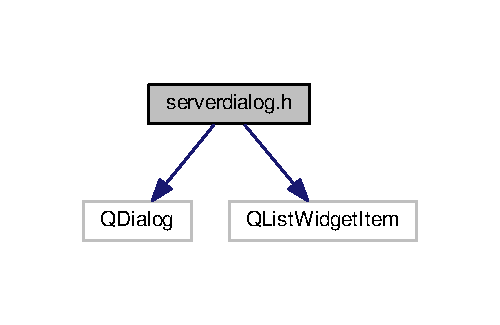
\includegraphics[width=240pt]{serverdialog_8h__incl}
\end{center}
\end{figure}
This graph shows which files directly or indirectly include this file\+:
\nopagebreak
\begin{figure}[H]
\begin{center}
\leavevmode
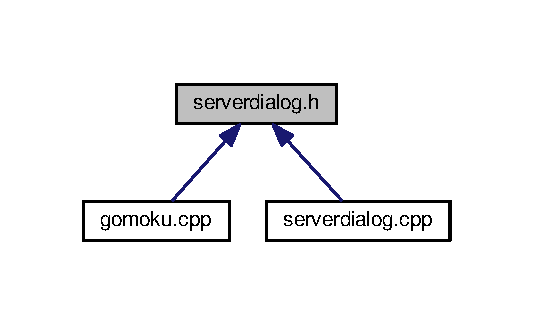
\includegraphics[width=256pt]{serverdialog_8h__dep__incl}
\end{center}
\end{figure}
\subsection*{Classes}
\begin{DoxyCompactItemize}
\item 
class \hyperlink{classServerDialog}{Server\+Dialog}
\begin{DoxyCompactList}\small\item\em Dialog to setup a server. \end{DoxyCompactList}\end{DoxyCompactItemize}
\subsection*{Namespaces}
\begin{DoxyCompactItemize}
\item 
 \hyperlink{namespaceUi}{Ui}
\end{DoxyCompactItemize}

%--- End generated contents ---

% Index
\backmatter
\newpage
\phantomsection
\clearemptydoublepage
\addcontentsline{toc}{chapter}{Index}
\printindex

\end{document}
